\chapter{فرانت‌اند}
    \section{ساختار راهنمای وب‌سایت}
    این راهنما به شما کمک می‌کند تا با تمام بخش‌های وب‌سایت آشنا شوید و بتوانید از قابلیت‌های آن به‌طور کامل استفاده کنید. وب‌سایت Polaris با هدف ارائه‌ی یک بستر کاربرپسند و تعاملی طراحی شده است که کاربران را قادر می‌سازد تا اطلاعات شبکه را مشاهده کرده، گزارش‌ها را بررسی کنند و به ابزارهای مدیریتی پیشرفته دسترسی داشته باشند.  
    راهنما به‌گونه‌ای ساختار یافته که شما از اولین ورود به صفحه‌ی اصلی تا استفاده از امکانات پیشرفته، مسیر مشخصی را دنبال کنید. در هر بخش، توضیحات همراه با مراحل عملی ارائه شده‌اند تا تجربه‌ی استفاده شما روان و بدون ابهام باشد.  
    \section{شروع به کار}
    \begin{itemize}
    	\item  معرفی کوتاهی از وب‌سایت و عملکردهای کلیدی آن: وب‌سایت Polaris یک پلتفرم تحت وب برای مدیریت، مانیتورینگ و تحلیل داده‌های شبکه است. این سامانه با رابط کاربری ساده و مدرن، امکاناتی همچون مشاهده‌ی نقشه‌ی پوشش، بررسی وضعیت لحظه‌ای شبکه، دسترسی به گزارش‌های دقیق و استفاده از ابزارهای مدیریتی را فراهم می‌کند. هدف اصلی این وب‌سایت، ارائه‌ی اطلاعات دقیق و به‌روز به کاربران، همراه با تجربه‌ی کاربری سریع و کارآمد است. این وب‌سایت در آدرس \url{https://polaris.work.gd/} قرار گرفته است.
    	\item  صفحه فرود: صفحه فرود وب‌سایت \lr{Polaris} به‌گونه‌ای طراحی شده است که کاربران بتوانند در اولین نگاه با عملکردها و امکانات کلیدی سامانه آشنا شوند. این صفحه شامل چندین بخش اصلی است که هرکدام نقش ویژه‌ای در هدایت کاربر و ارائه اطلاعات دارند.

        \begin{itemize}
            \item \textbf{هدر و نوار ناوبری:}  
            در بالای صفحه، نوار ناوبری قرار دارد که شامل لوگوی \lr{Polaris} و دکمه‌های دسترسی سریع به بخش‌های \lr{Features}، \lr{FAQ}، \lr{Download} و داشبورد است. کاربران همچنین می‌توانند از منوی همبرگری (\lr{Menu}) برای دسترسی به این بخش‌ها در نمایشگرهای کوچک استفاده کنند. این نوار ناوبری با طراحی شفاف و افکت \lr{backdrop blur}، تجربه‌ای مدرن و کاربرپسند ارائه می‌دهد.
        
            \item \textbf{بخش معرفی:}  
            این بخش شامل عنوان اصلی، توضیحات کوتاه و دکمه‌های فراخوان است. تصویر یک گوشی موبایل در کنار متن، محیط اپلیکیشن و نمایش تحلیل شبکه را نشان می‌دهد. این طراحی باعث جلب توجه کاربر و هدایت او به اقدامات کلیدی مانند دانلود برنامه می‌شود.  
            \begin{center}
                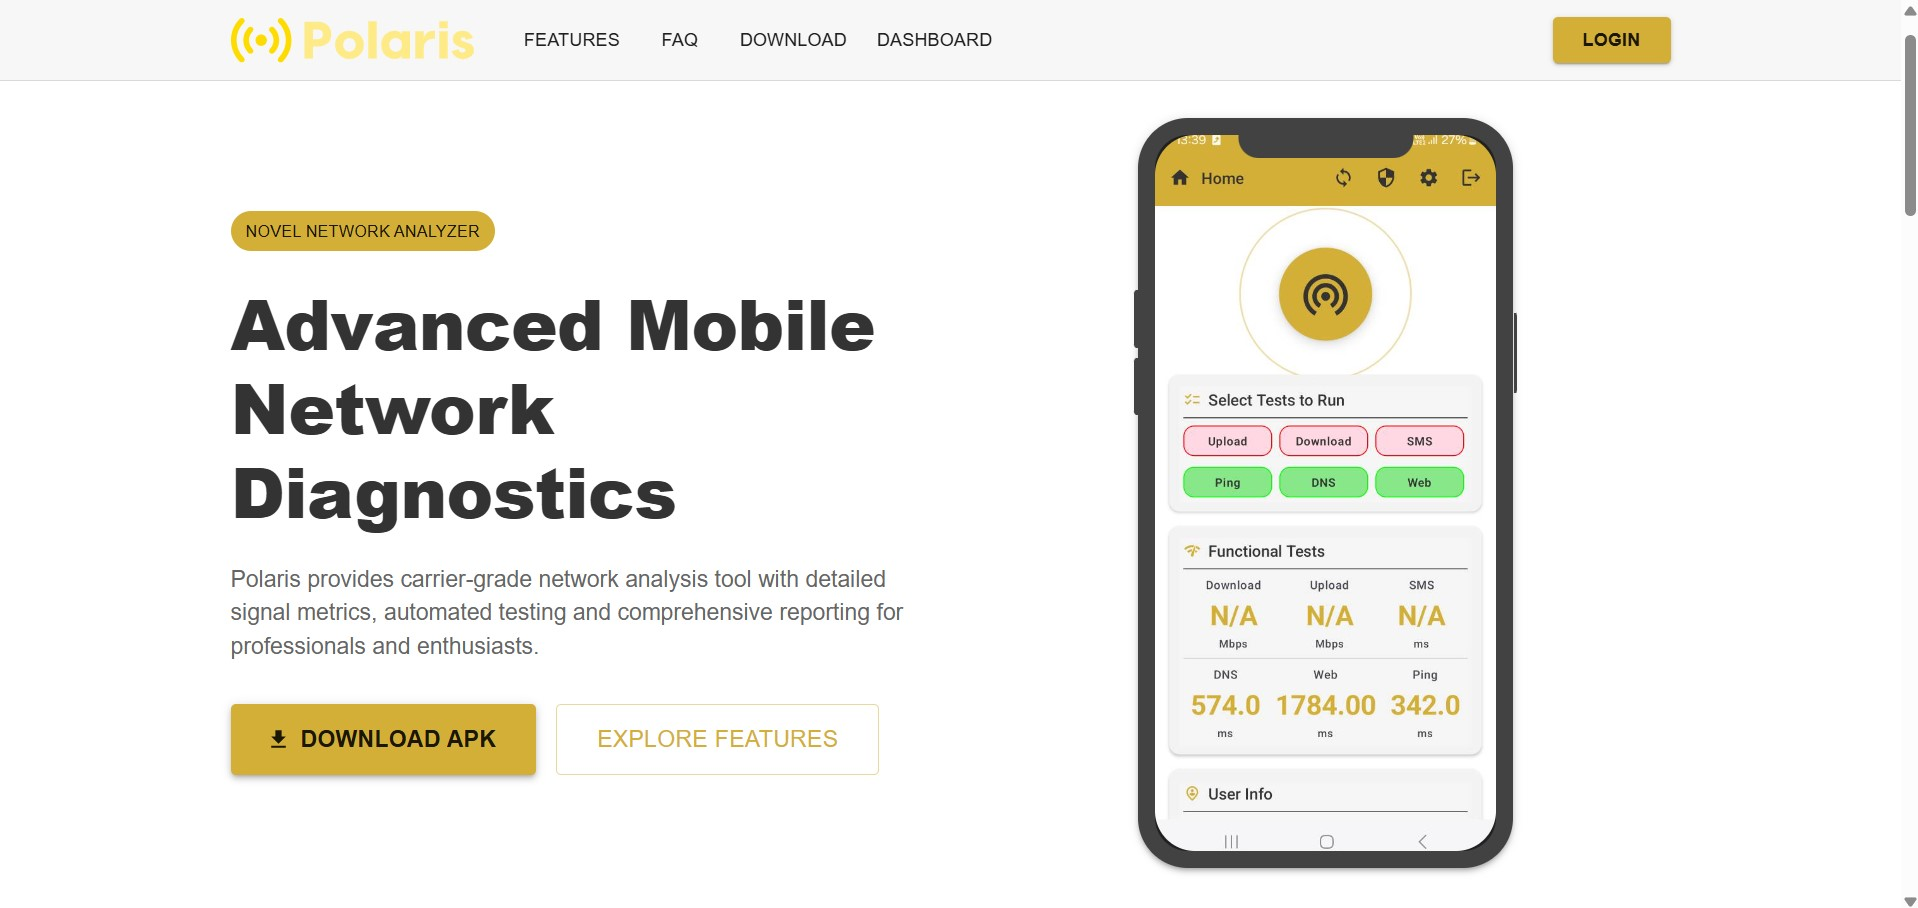
\includegraphics[width=0.9\textwidth]{images/fr_hero.jpg}
            \end{center}
        
            \item \textbf{ویژگی‌ها:}  
            این بخش شامل کارت‌هایی است که ویژگی‌های کلیدی اپلیکیشن را نمایش می‌دهند. هر کارت شامل یک آیکون، عنوان و توضیح مختصر است. ویژگی‌هایی مانند تحلیل شبکه موبایل، گزارش‌گیری دقیق و ابزارهای تست پیشرفته در این بخش معرفی شده‌اند.  
            \begin{center}
                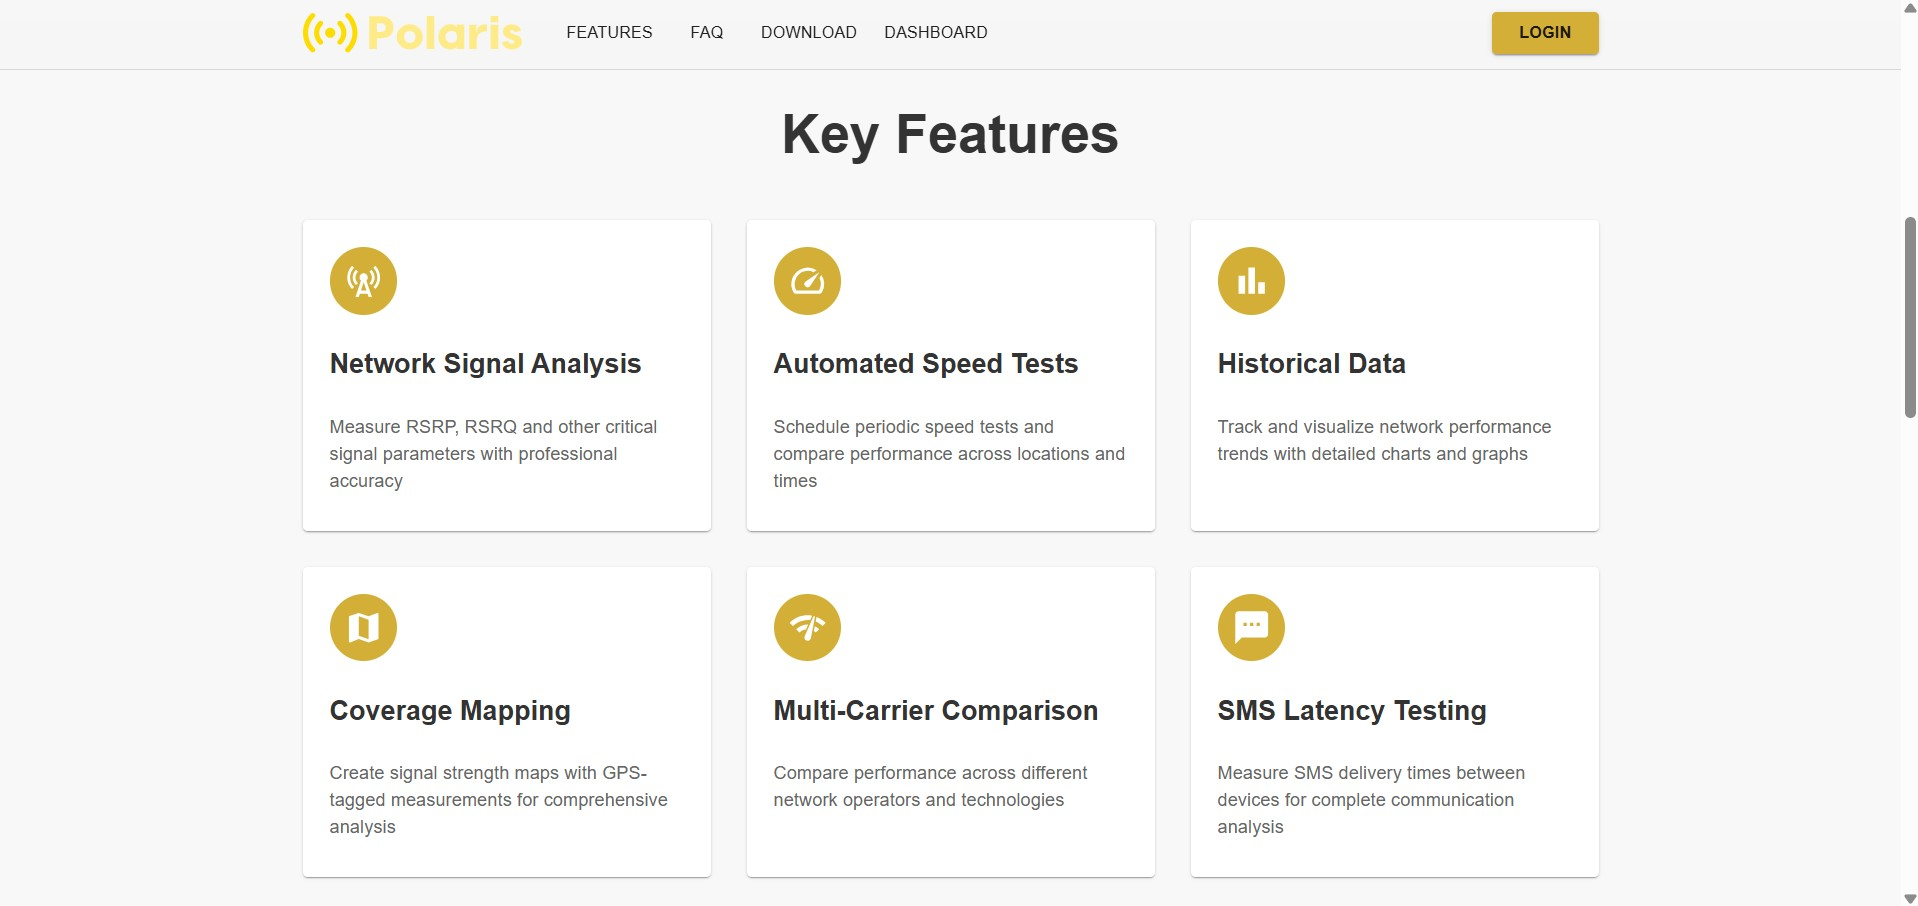
\includegraphics[width=0.9\textwidth]{images/fr_features.jpg}
            \end{center}
        
            \item \textbf{سوالات متداول:}  
            این بخش شامل پرسش‌ها و پاسخ‌های متداول کاربران است. هر پرسش در قالب یک \lr{Accordion} ارائه شده است که با کلیک روی آن، پاسخ مربوطه نمایش داده می‌شود. این طراحی باعث دسترسی سریع به اطلاعات و کاهش سردرگمی کاربر می‌شود.  
            \begin{center}
                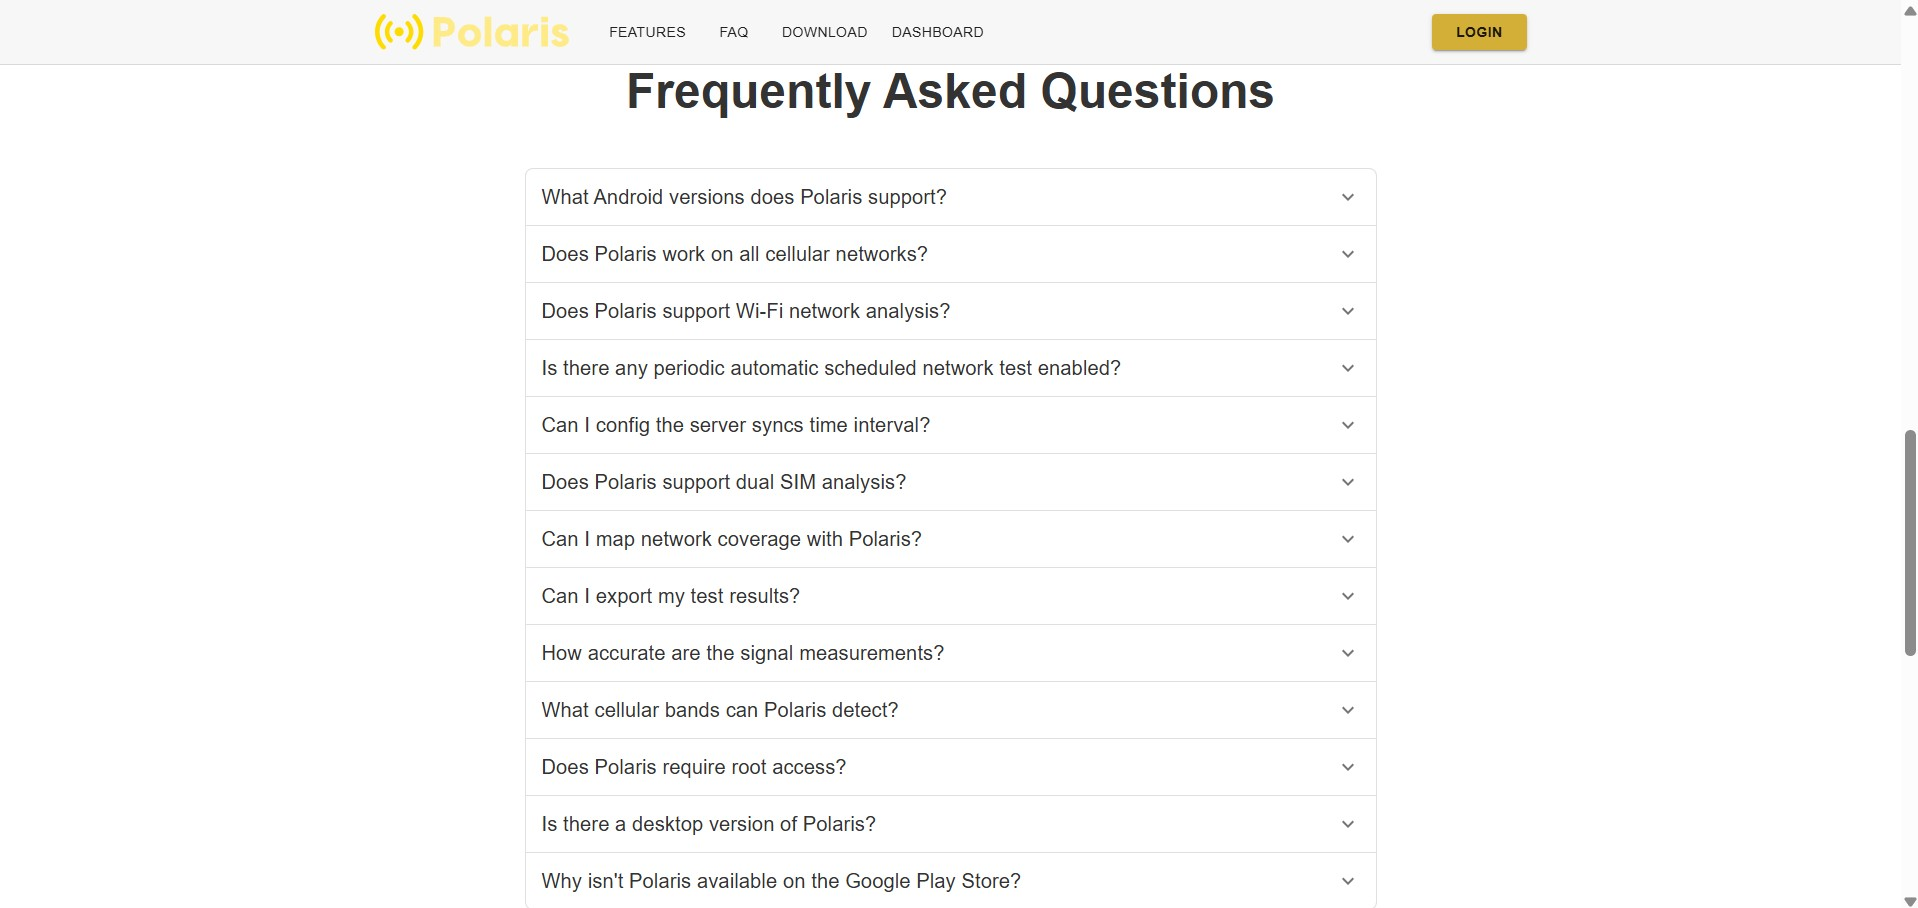
\includegraphics[width=0.9\textwidth]{images/fr_faq.jpg}
            \end{center}
        
            \item \textbf{دانلود:}  
            کاربران می‌توانند آخرین نسخه اپلیکیشن \lr{Polaris} را از این بخش دانلود کنند. اطلاعات نسخه، تاریخ انتشار، حجم فایل و پیش‌نیازها در قالب یک پنل مشخص نمایش داده شده‌اند. همچنین راهنمای نصب گام‌به‌گام ارائه شده است که شامل فعال‌سازی نصب از منابع ناشناس، نصب فایل \lr{APK} و راه‌اندازی اپلیکیشن است.  با کلیک بر روی دکمه \lr{DOWNLOAD NOW} اپلیکیشن دانلود می‌شود.
            \begin{center}
                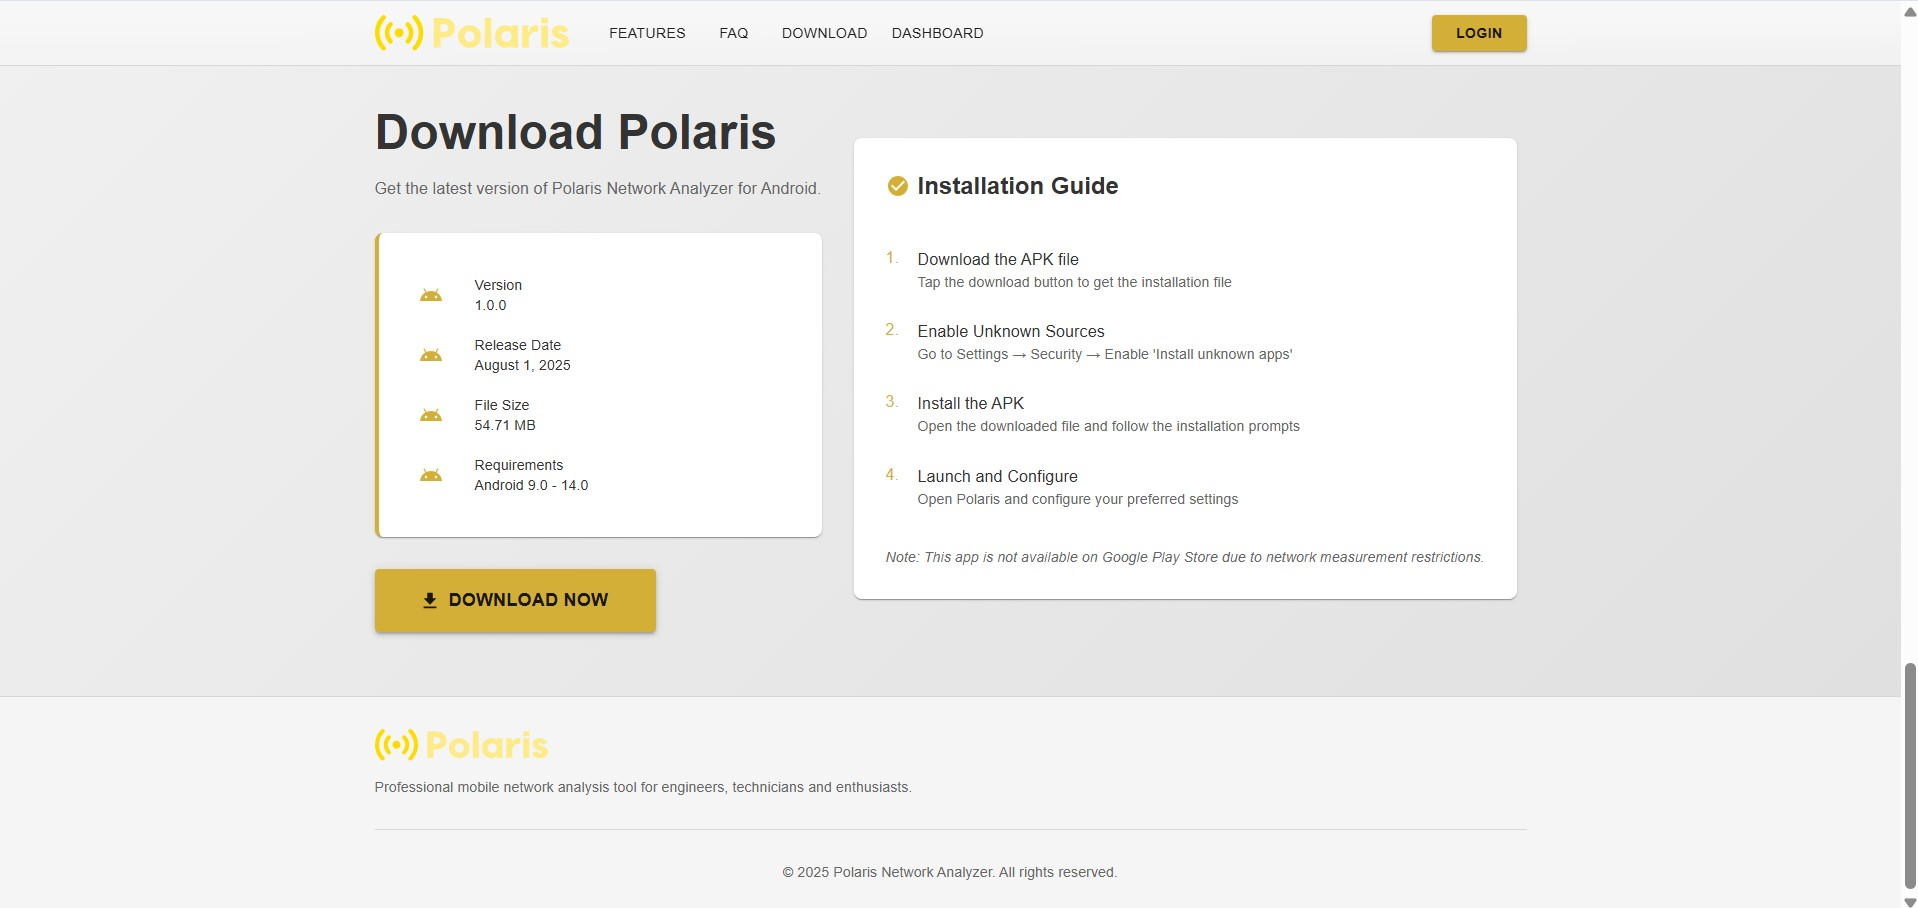
\includegraphics[width=0.9\textwidth]{images/fr_download.jpg}
            \end{center}
        
            \item \textbf{پاورقی و کپی‌رایت:}  
            در انتهای صفحه، لوگوی \lr{Polaris} و اطلاعات کپی‌رایت نمایش داده شده‌اند که حس اطمینان و هویت برند را به کاربران منتقل می‌کند.
        \end{itemize}
        
        این طراحی صفحه فرود، با ترکیب بخش‌های بصری و متنی، کاربر را به طور طبیعی به سمت بخش‌های مهم وب‌سایت هدایت کرده و تجربه کاربری روان و جذابی ارائه می‌دهد.

    \end{itemize}
    \section{مدیریت حساب کاربری}
    \begin{itemize}
    	\item \textbf{ثبت‌نام:} برای ایجاد حساب کاربری در نسخه تحت‌وب \lr{Polaris}، در صفحه اصلی وب‌سایت روی دکمه \lr{Login} کلیک کنید:
	    	\begin{center}
	    		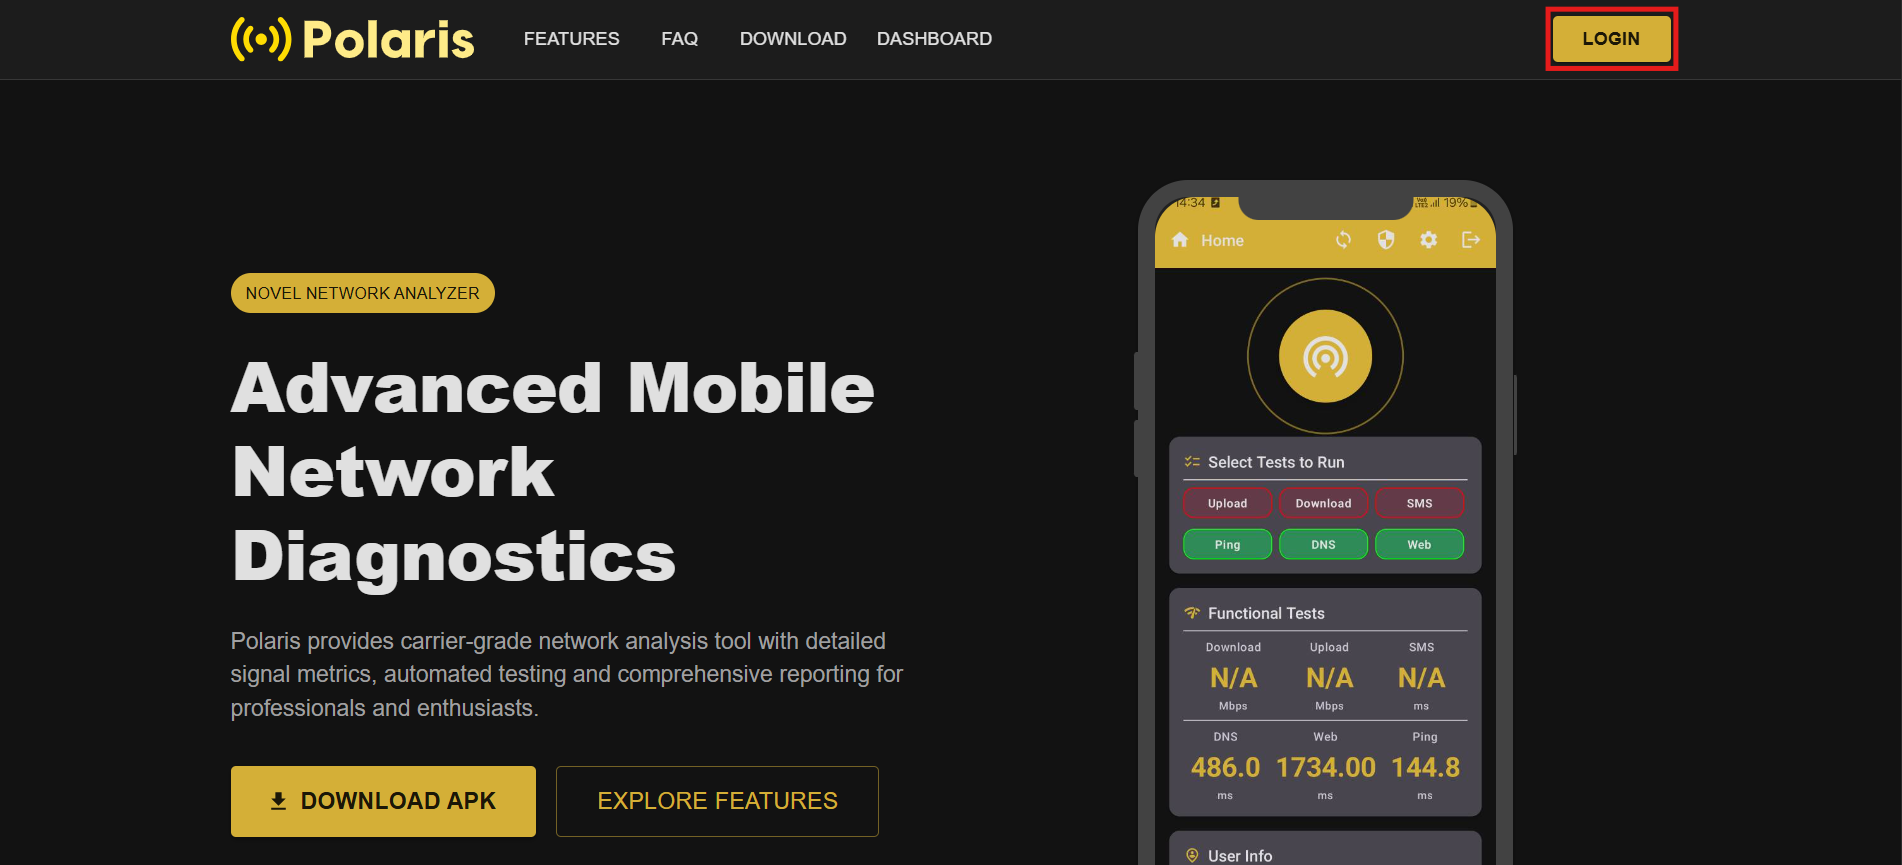
\includegraphics[width=\textwidth]{images/fr-landing.png}
	    	\end{center}
    	سپس به صفحه زیر منتقل می‌شوید که در این صفحه نیز نیاز است بر روی لینک \lr{Sign Up} کلیک کنید:
    		\begin{center}
    			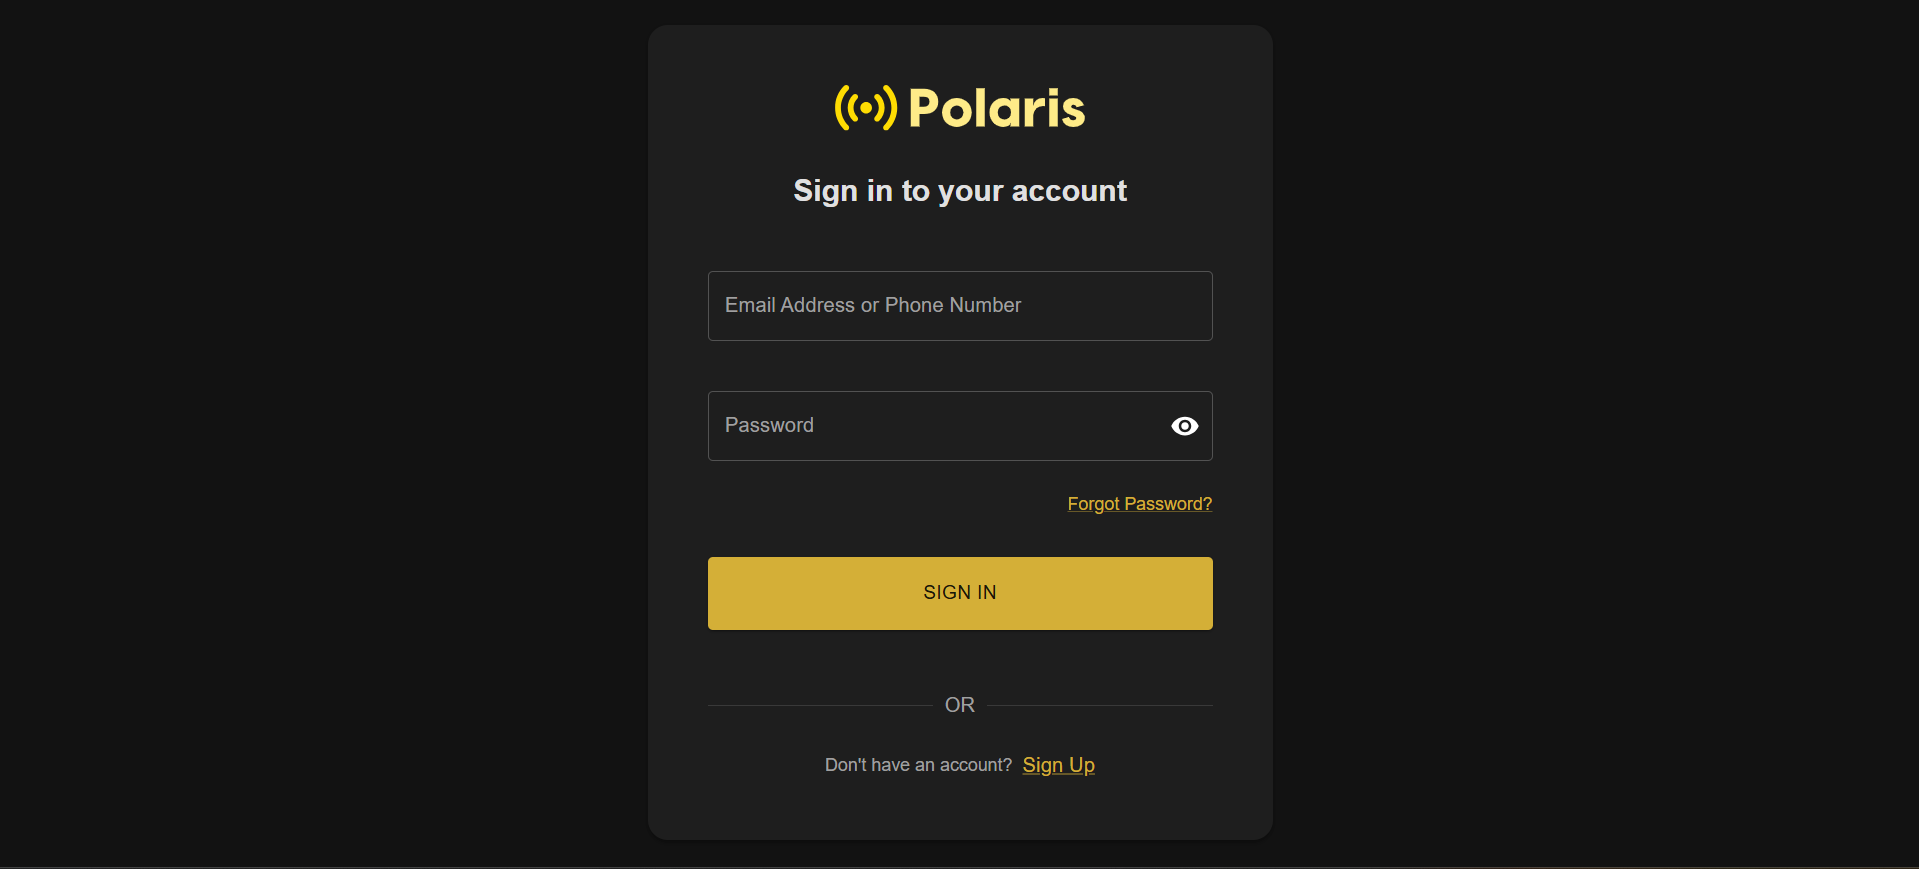
\includegraphics[width=\textwidth]{images/fr-login-empty.png}
    		\end{center} 
    		پس از کلیک بر روی لینک \lr{Sign Up} به صفحه زیر منتقل می‌شوید:
    		\begin{center}
    			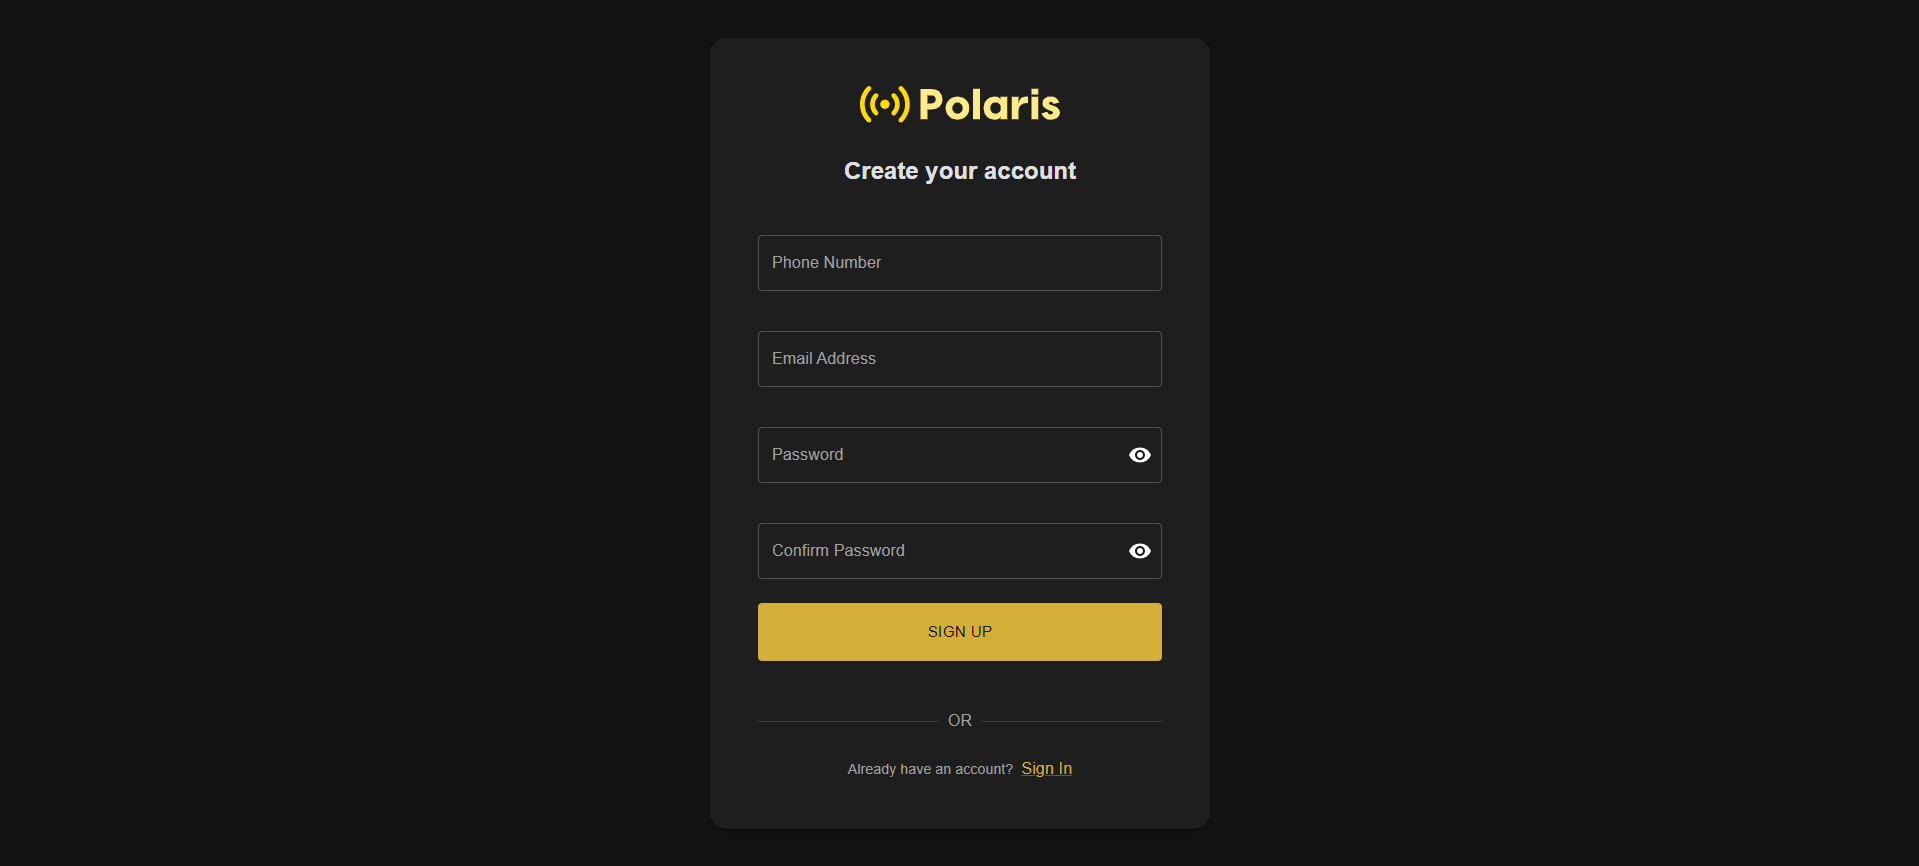
\includegraphics[width=\textwidth]{images/fr-signup-empty.png}
    		\end{center}
    		در این صفحه در صورت تمایل و داشتن حساب می‌توانید به صفحه Login برگردید.
    	\begin{itemize}
    		\item \textbf{پر کردن فرم ثبت‌نام:}  
    		در این صفحه، اطلاعات خواسته‌شده شامل پست الکترونیک، شماره تلفن همراه و گذرواژه را وارد کنید. شماره همراه باید به فرمت \lr{09xxxxxxxxx} و گذرواژه باید حداقل 8 کاراکتر (شامل حروف و اعداد) باشد. پس از تکمیل فرم، روی دکمه \lr{Sign Up} کلیک کنید. در صورت وجود خطا، پیام مناسب نمایش داده می‌شود و در غیر این صورت، پیام موفقیت آمیز بودن نمایش داده می‌شود:
    			\begin{center}
    				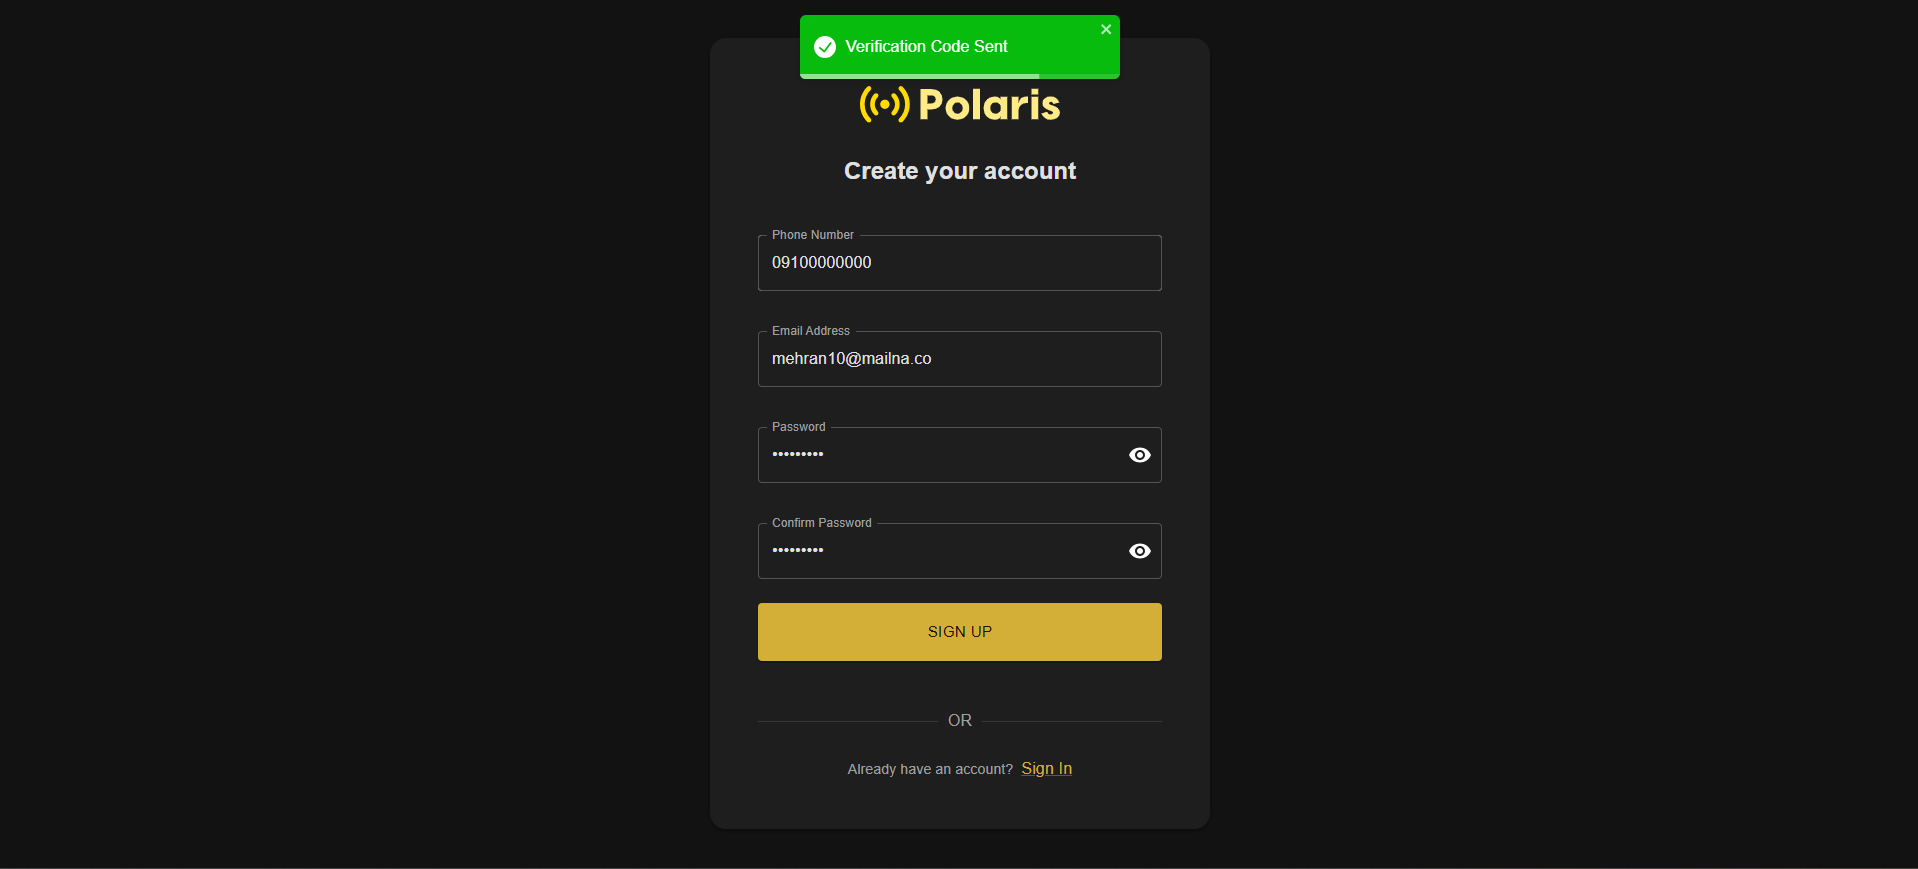
\includegraphics[width=\textwidth]{images/fr-signup-success.png}
    			\end{center}
    		\item \textbf{تأیید آدرس ایمیل:}  
    		پس از ارسال فرم ثبت‌نام، در صورت موفقیت آمیز بودن به صفحه تأیید منتقل می‌شوید:
    		\begin{center}
    			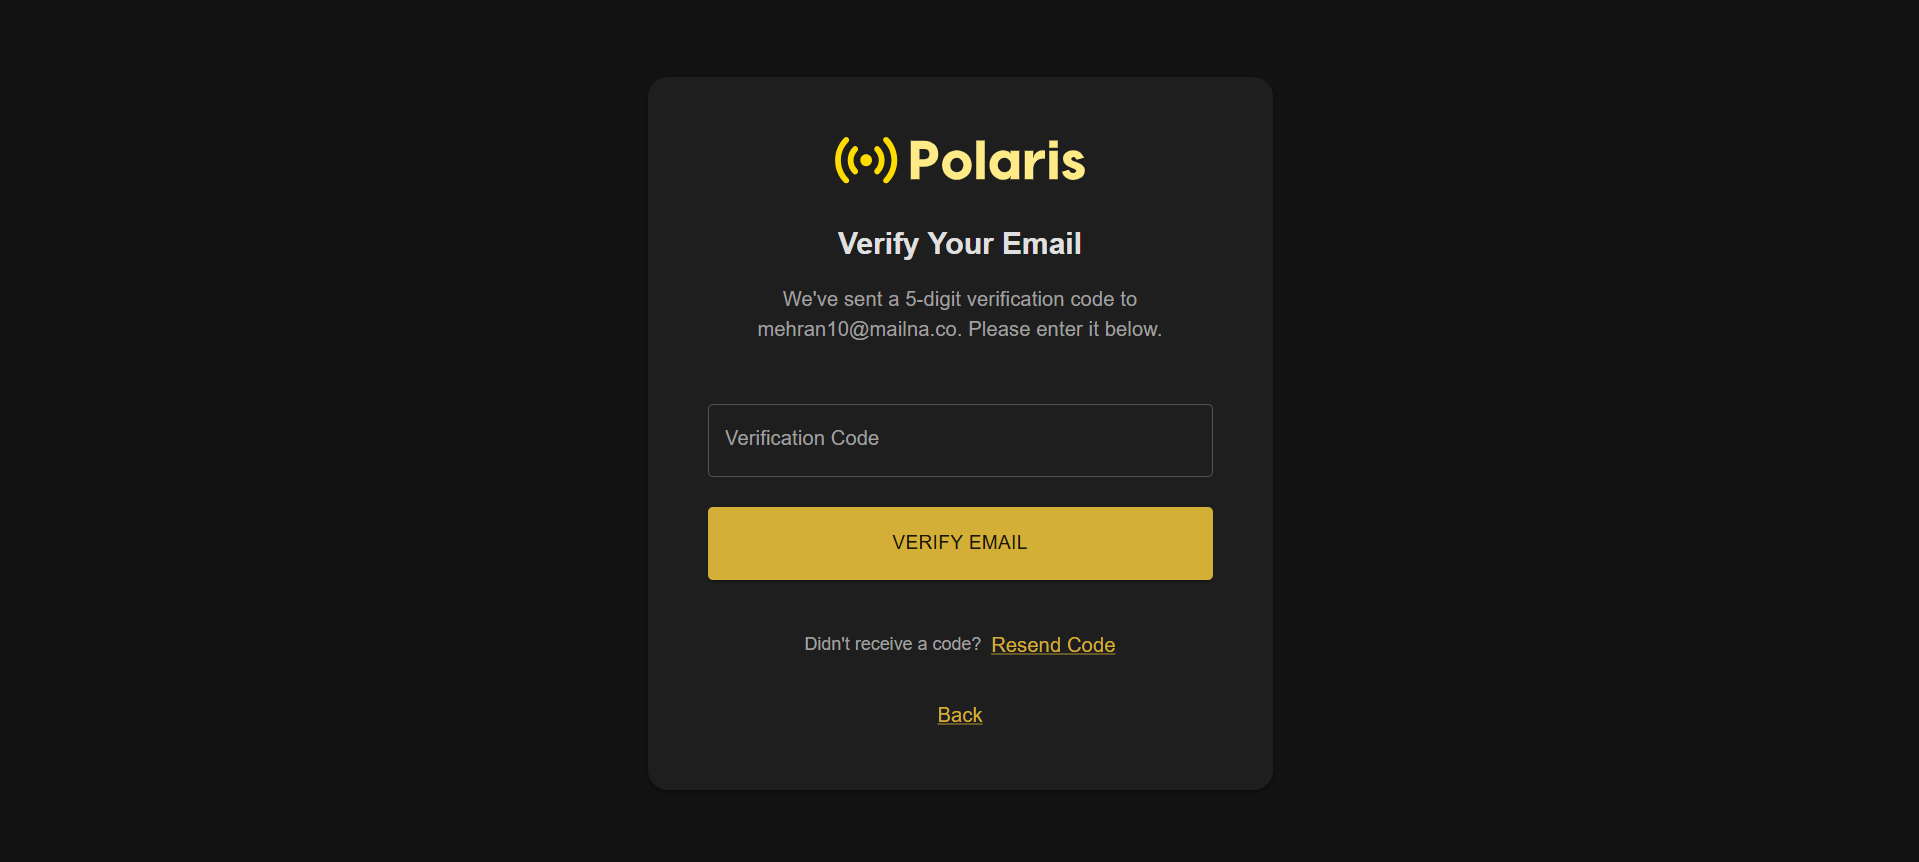
\includegraphics[width=\textwidth]{images/fr-verify-empty.png}
    		\end{center}
    		در این بخش، کد ۵ رقمی ارسال‌شده به ایمیلی که در مرحله قبل وارد کرده‌اید را وارد کنید. در صورت عدم دریافت کد، می‌توانید روی لینک \lr{Resend Code} کلیک کنید. همچنین، امکان بازگشت به صفحه ثبت‌نام با کلیک بر روی \lr{Back} وجود دارد.  
    		پس از وارد کردن کد صحیح، پیام موفقیت‌آمیز بودن ایجاد حساب نمایش داده شده و با یک تأخیر کوتاه به داشبورد منتقل می‌شوید:
    		\begin{center}
    			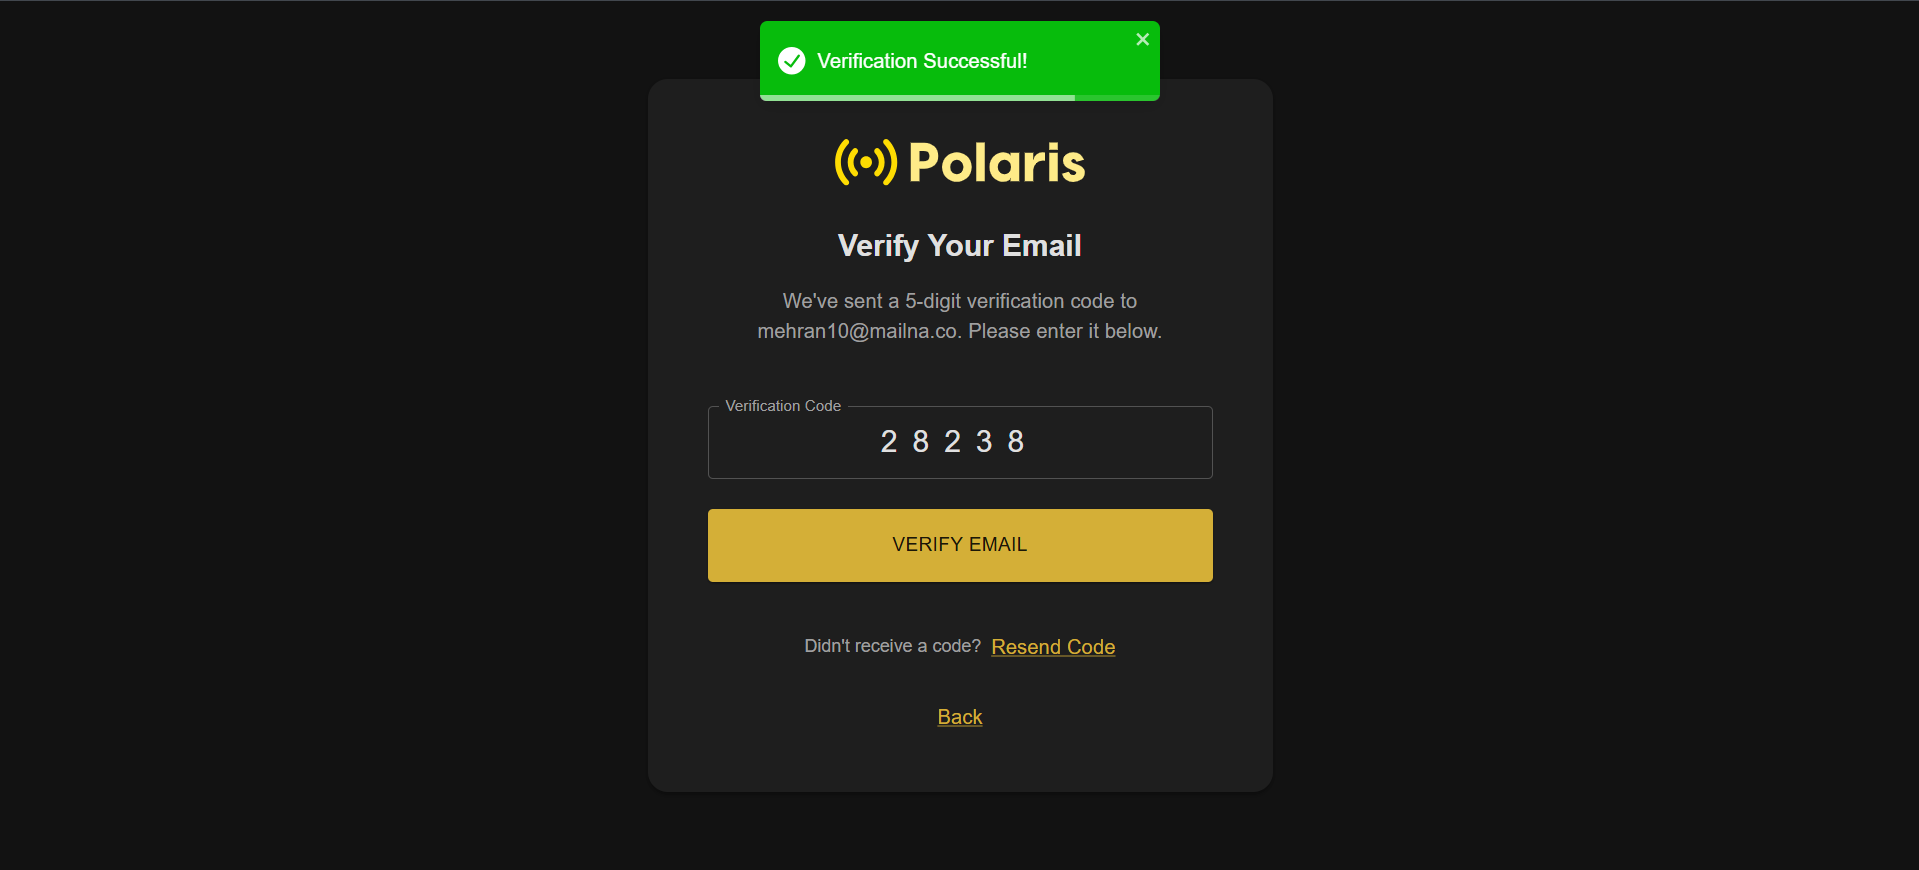
\includegraphics[width=\textwidth]{images/fr-verify-success.png}
    		\end{center}
    	\end{itemize}
    	
    	\item \textbf{ورود به حساب:}  
    	در صفحه ورود، پست الکترونیک یا شماره همراه و گذرواژه خود را وارد کرده و روی دکمه \lr{Login} کلیک کنید. در صورت وجود خطا (مانند رمز اشتباه)، پیام مناسب نمایش داده می‌شود. اگر ایمیل شما هنوز تأیید نشده باشد، سیستم شما را به صفحه تأیید هدایت خواهد کرد. در صورت موفقیت، پس از نمایش پیام زیر وارد داشبورد خواهید شد:
    	\begin{center}
    		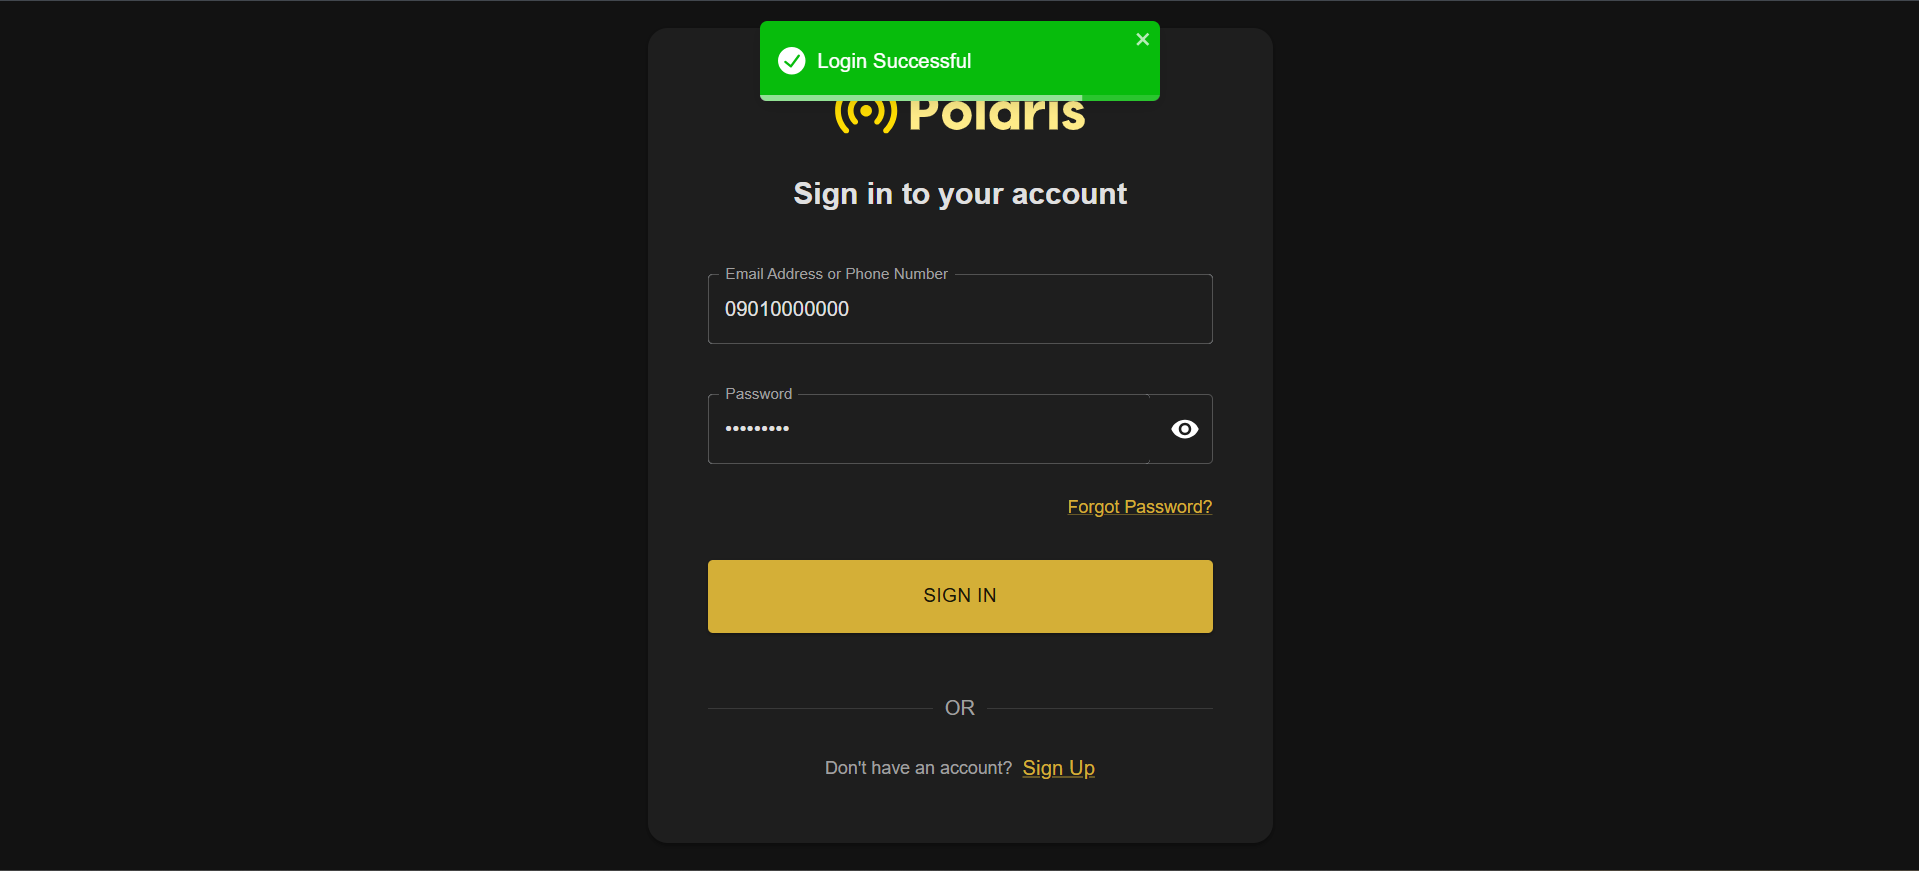
\includegraphics[width=\textwidth]{images/fr-login-success.png}
    	\end{center}
    	
    	\item \textbf{بازنشانی رمز عبور:}  
    	در صفحه ورود، با کلیک بر روی لینک \lr{Forgot Password?} به صفحه بازنشانی رمز عبور هدایت می‌شوید:
	    	\begin{center}
	    		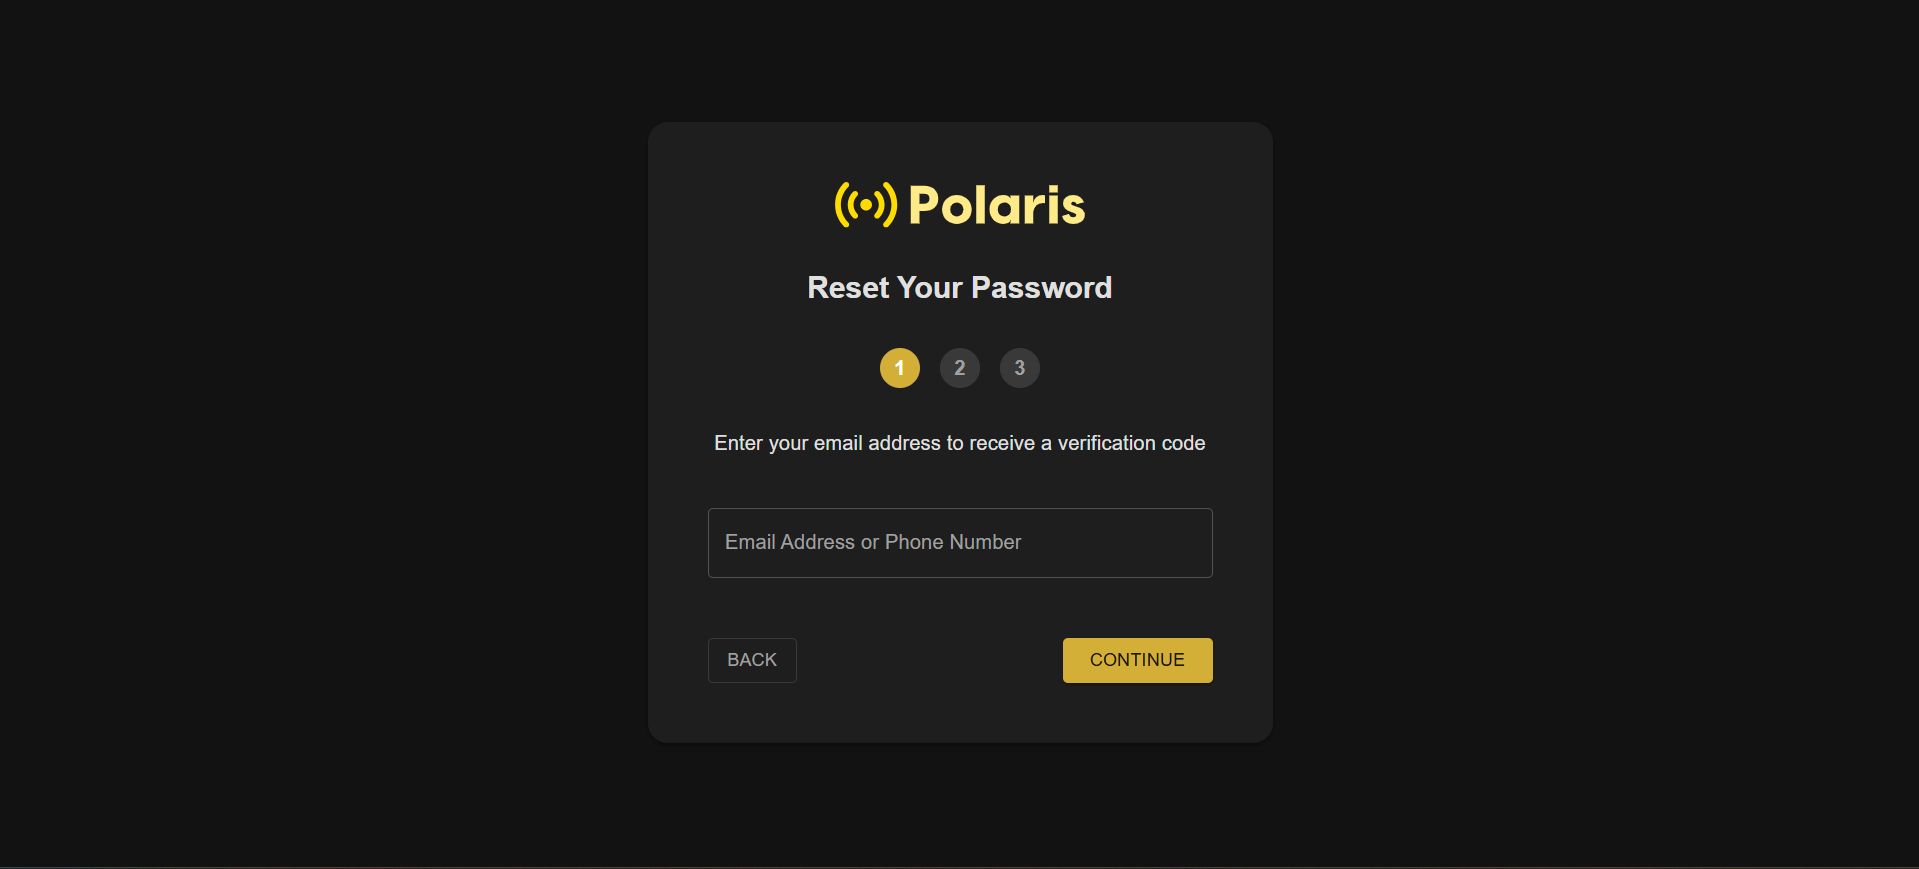
\includegraphics[width=\textwidth]{images/fr-reset-pass-empty.png}
	    	\end{center}
    	فرآیند بازنشانی رمز عبور شامل سه مرحله است:
    	\begin{itemize}
    		\item \textbf{مرحله ۱ (احراز هویت):}  
    		پست الکترونیک یا شماره همراه خود را وارد کرده و روی \lr{Send Code} کلیک کنید تا کد تأیید به ایمیل شما ارسال شود. در صورت موفقیت آمیز بودن این درخواست به مرحله بعدی می‌رویم و صفحه به صورت زیر خواهد شد:
    			\begin{center}
    				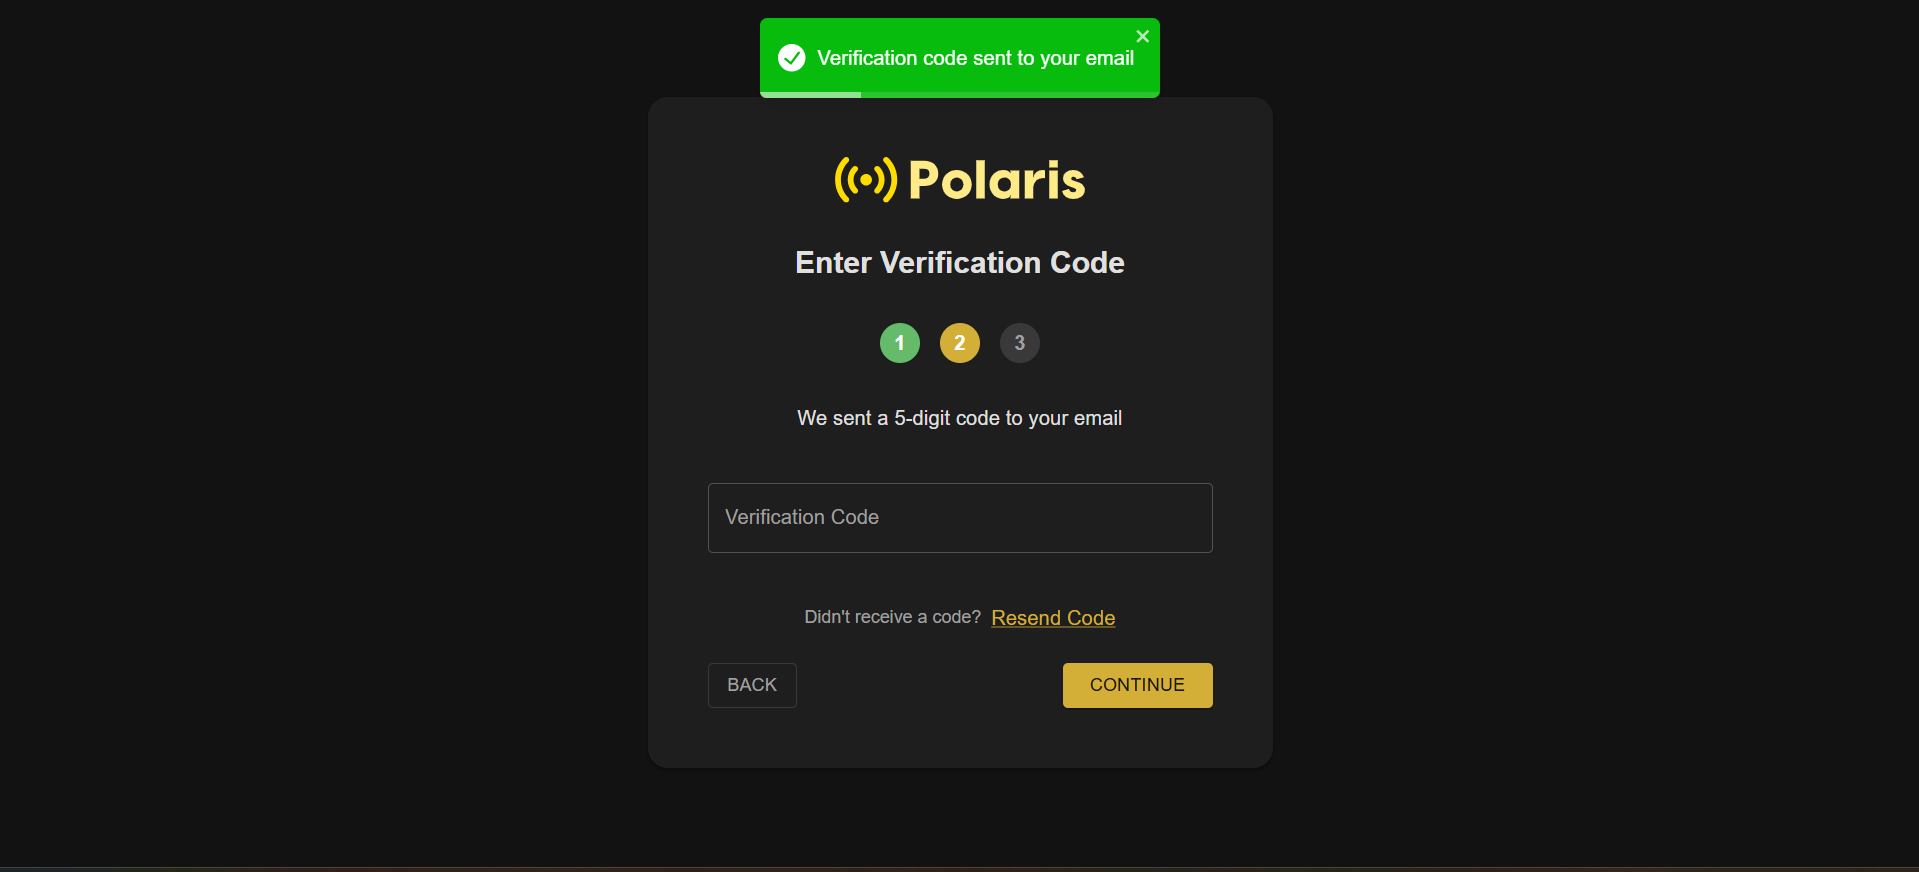
\includegraphics[width=\textwidth]{images/fr-verification-empty.png}
    			\end{center}
    		
    		\item \textbf{مرحله ۲ (تأیید):}  
    		در این مرحله کد ارسال‌شده به ایمیل را وارد کرده و روی \lr{Verify Code} کلیک کنید. امکان ارسال مجدد کد با \lr{Resend Code} یا بازگشت به مرحله قبل برای اصلاح اطلاعات  نیز وجود دارد. در صورت موفقیت آمیز بودن این درخواست صفحه به شکل زیر تغییر خواهد کرد:
    			\begin{center}
    				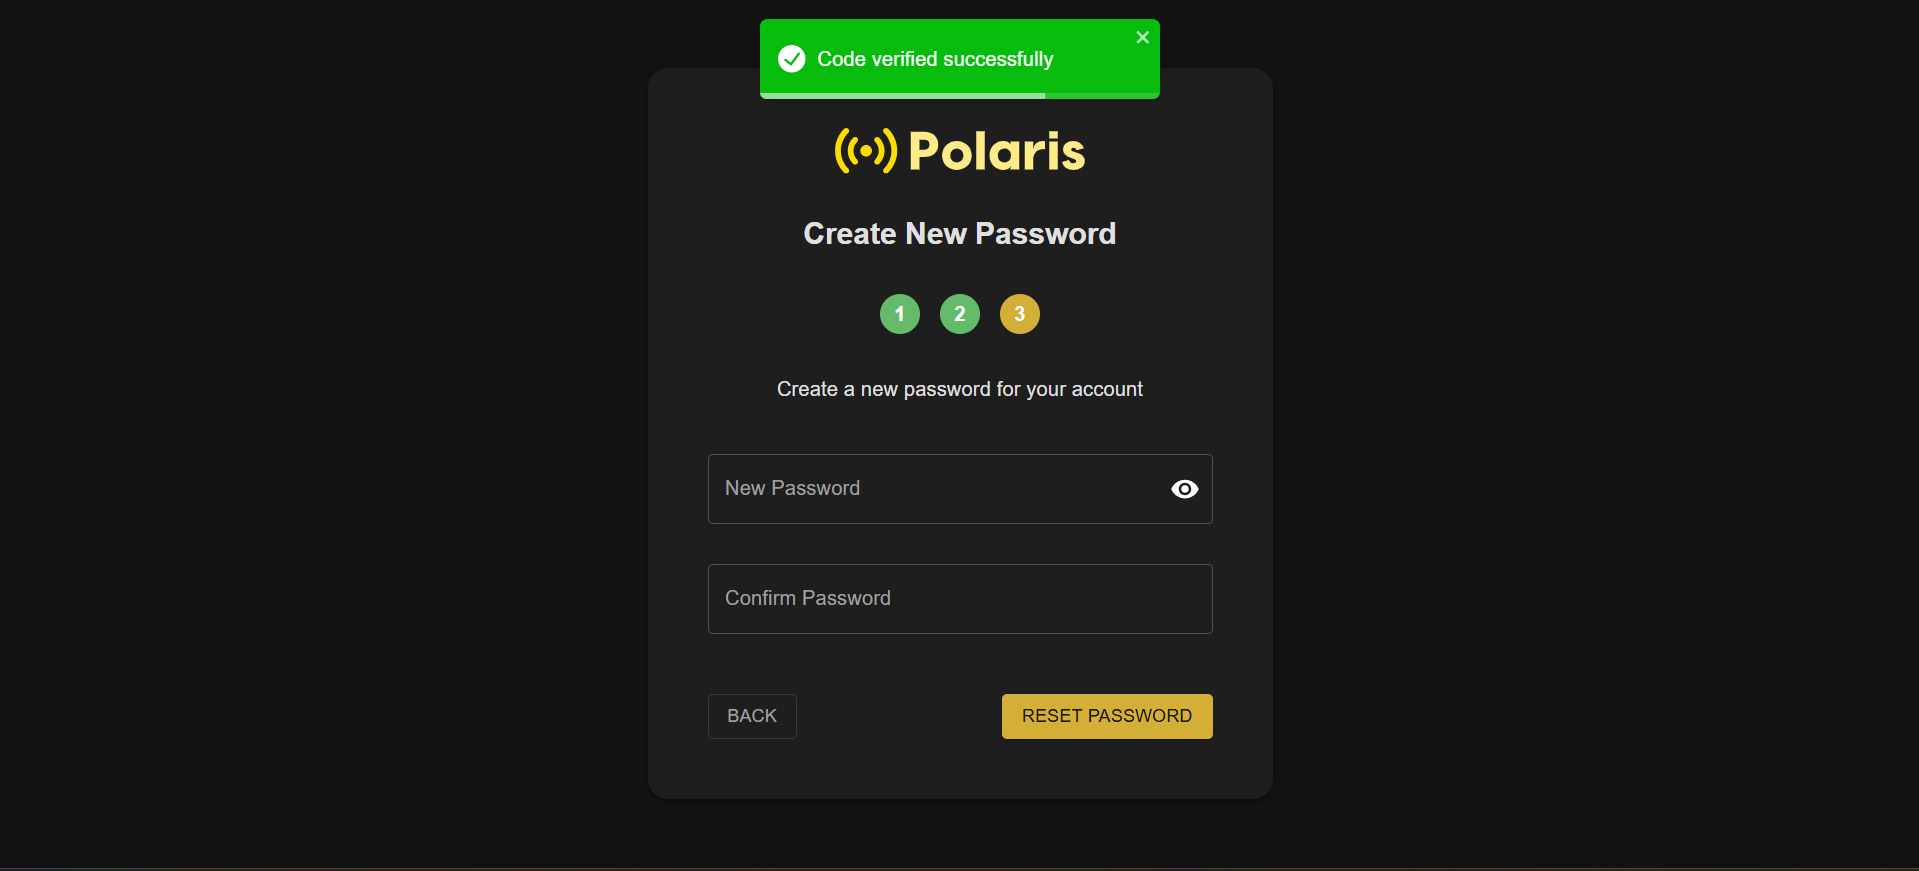
\includegraphics[width=\textwidth]{images/fr-new-pass-empty.png}
    			\end{center}
    		\item \textbf{مرحله ۳ (تغییر رمز عبور):}  
    		گذرواژه جدید (حداقل ۸ کاراکتر) را به همراه تکرار آن وارد کرده و روی \lr{Reset Password} کلیک کنید. پس از موفقیت، پیام زیر نمایش داده می‌شود و سپس به صفحه ورود منتقل خواهید شد:
		    	\begin{center}
		    		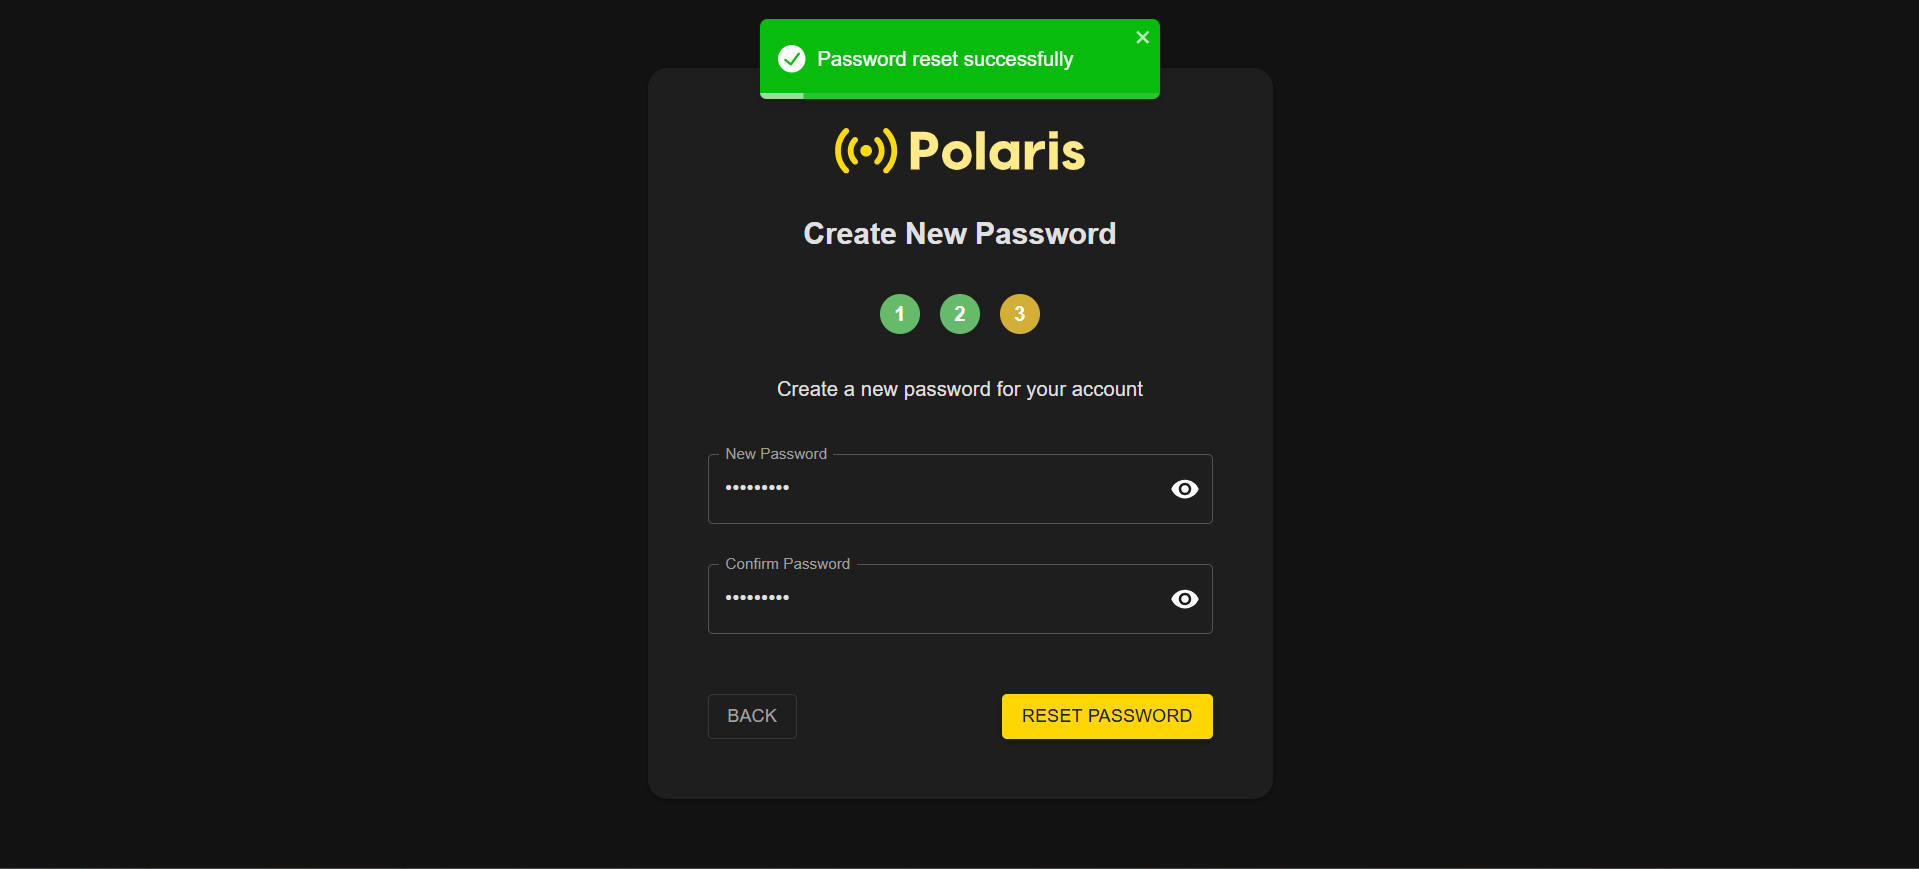
\includegraphics[width=\textwidth]{images/fr-new-pass-success.png}
		    	\end{center}
    	\end{itemize}
    \end{itemize}
    \section{بخش کاربری}
    \begin{itemize}
    	\item  مرور کلی داشبورد: پس از ورود به حساب در دفعه اول به دلیل نداشتن اطلاعات صفحه زیر را خواهید دید که فاقد اطلاعات می‌باشد:
    		\begin{center}
    			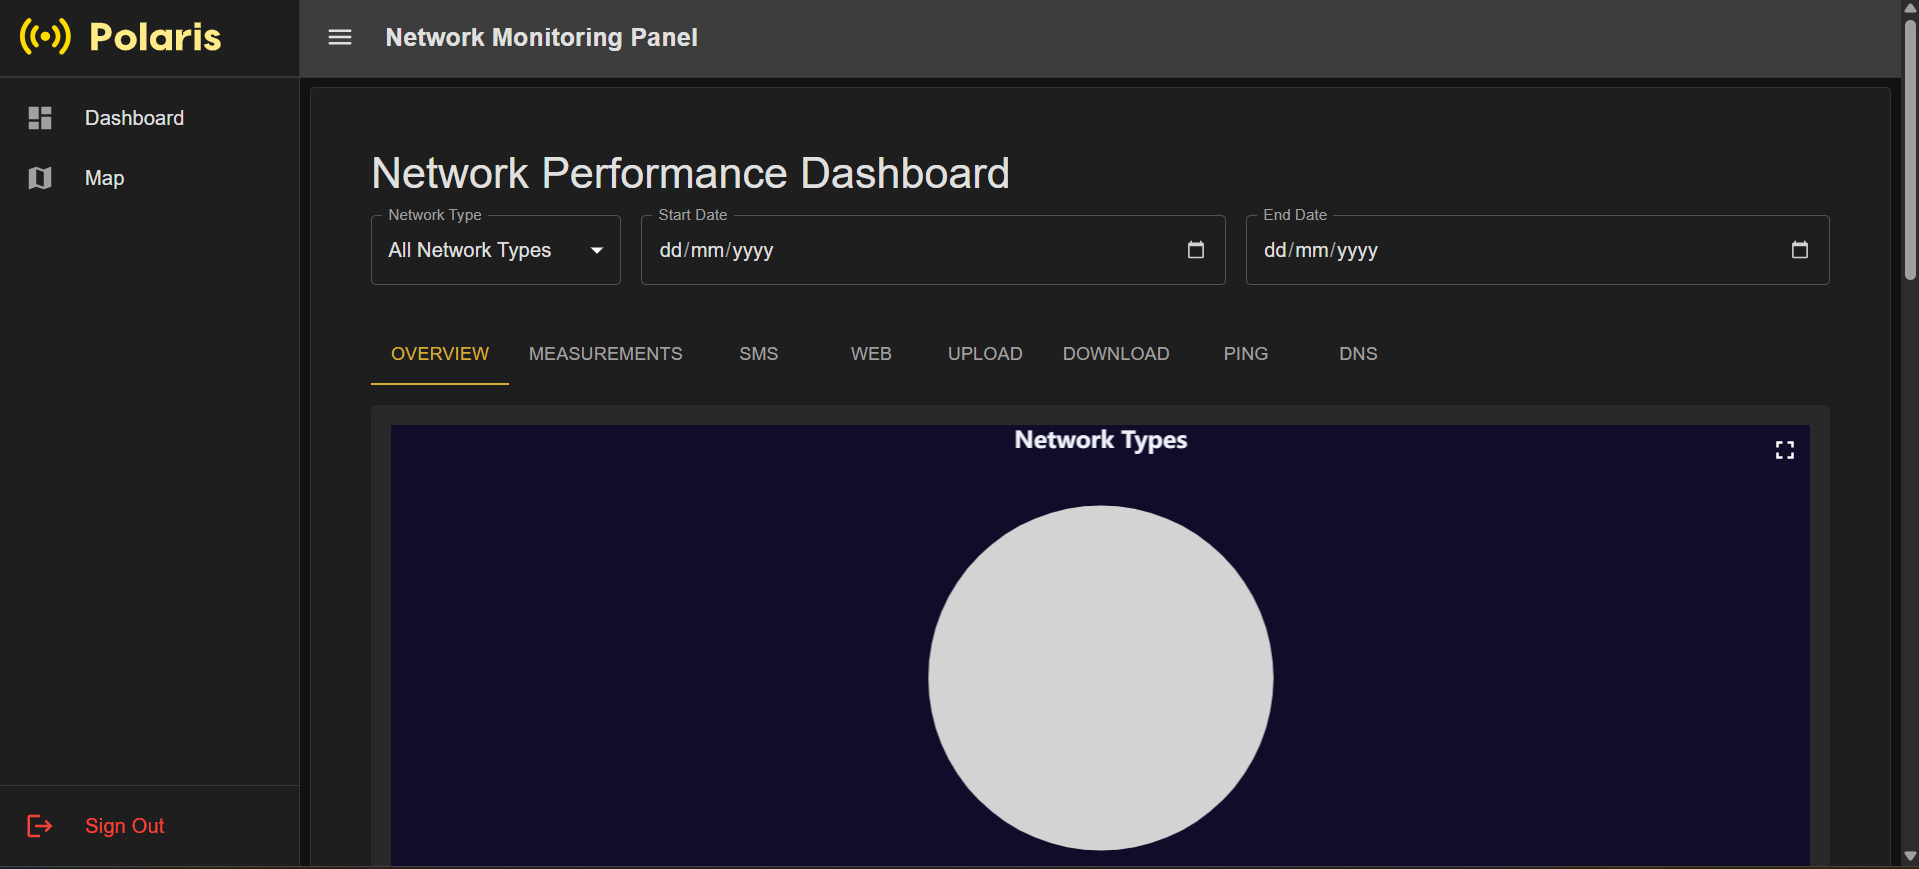
\includegraphics[width=\textwidth]{images/fr-dashboard-empty.png}
    		\end{center}
   		در صورت داشتن اطلاعات از پیش داشبورد به صورت زیر خواهد بود:
	   		\begin{center}
	   			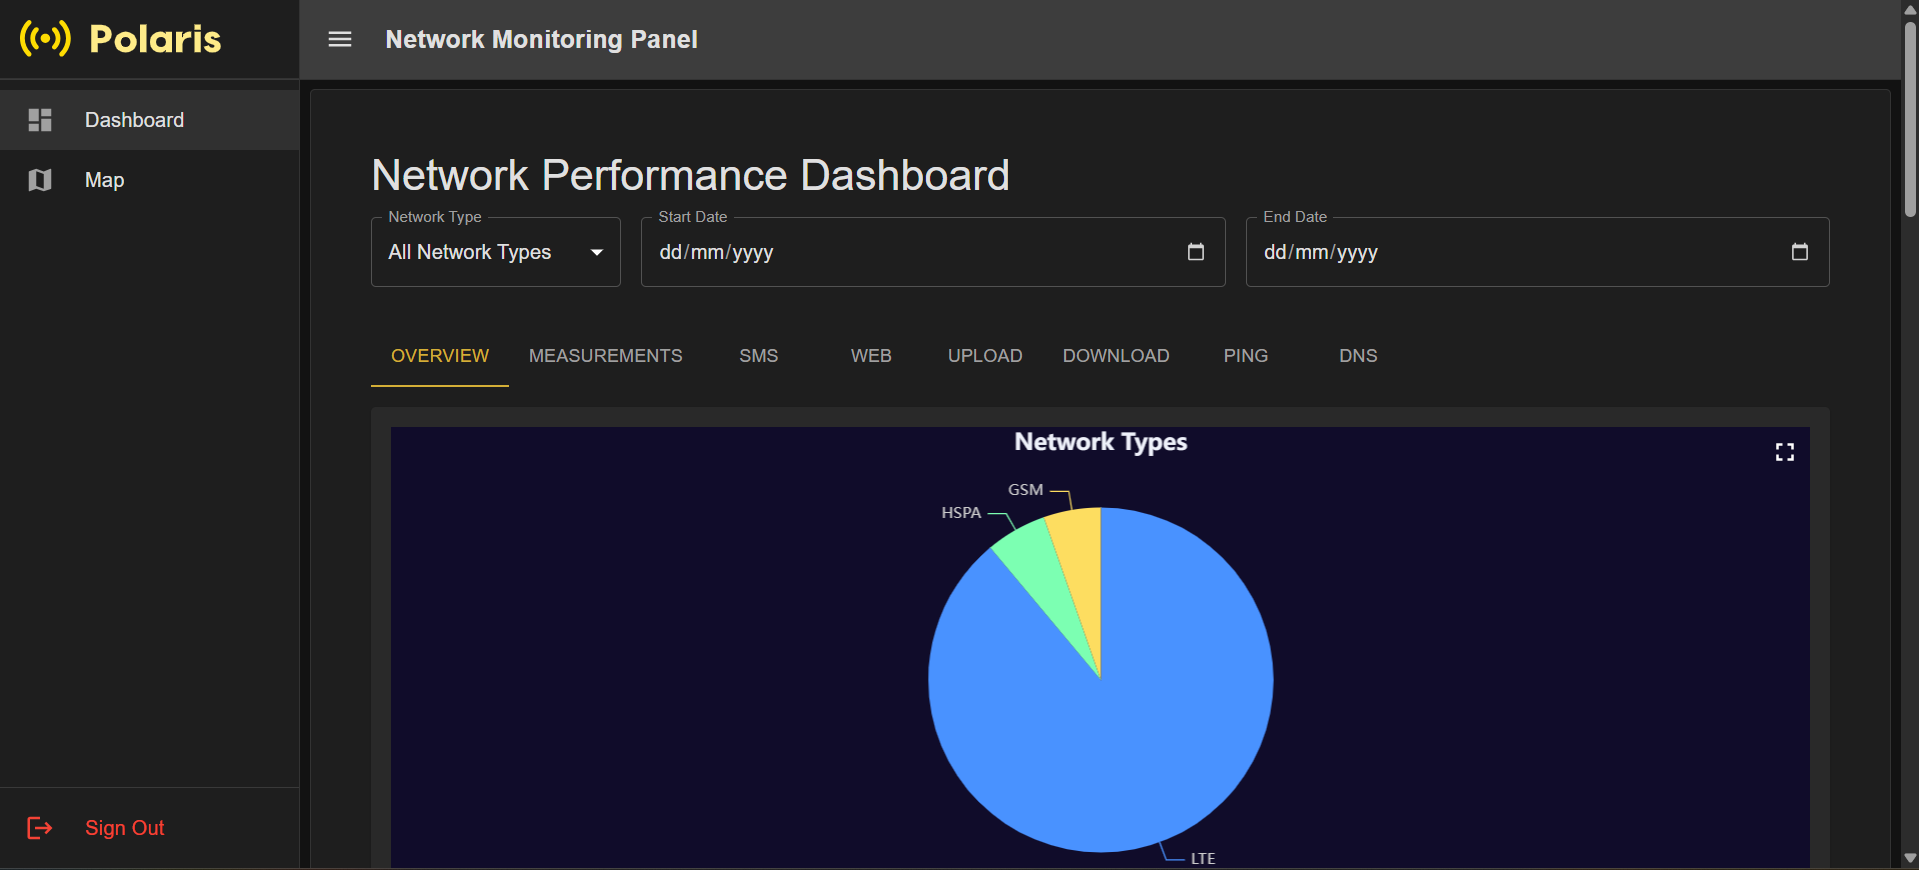
\includegraphics[width=\textwidth]{images/fr-dashboard-filled.png}
	   		\end{center}
	   	با کلیک بر روی آیکن سه خط در بالای سمت چپ که در تصویر زیر با کادر قرمز مشخص شده است نمای کناری سایت تا حدی پنهان می‌شود تا محتوای اصلی سایت بهتر نمایش داده شود:
	   		\begin{center}
				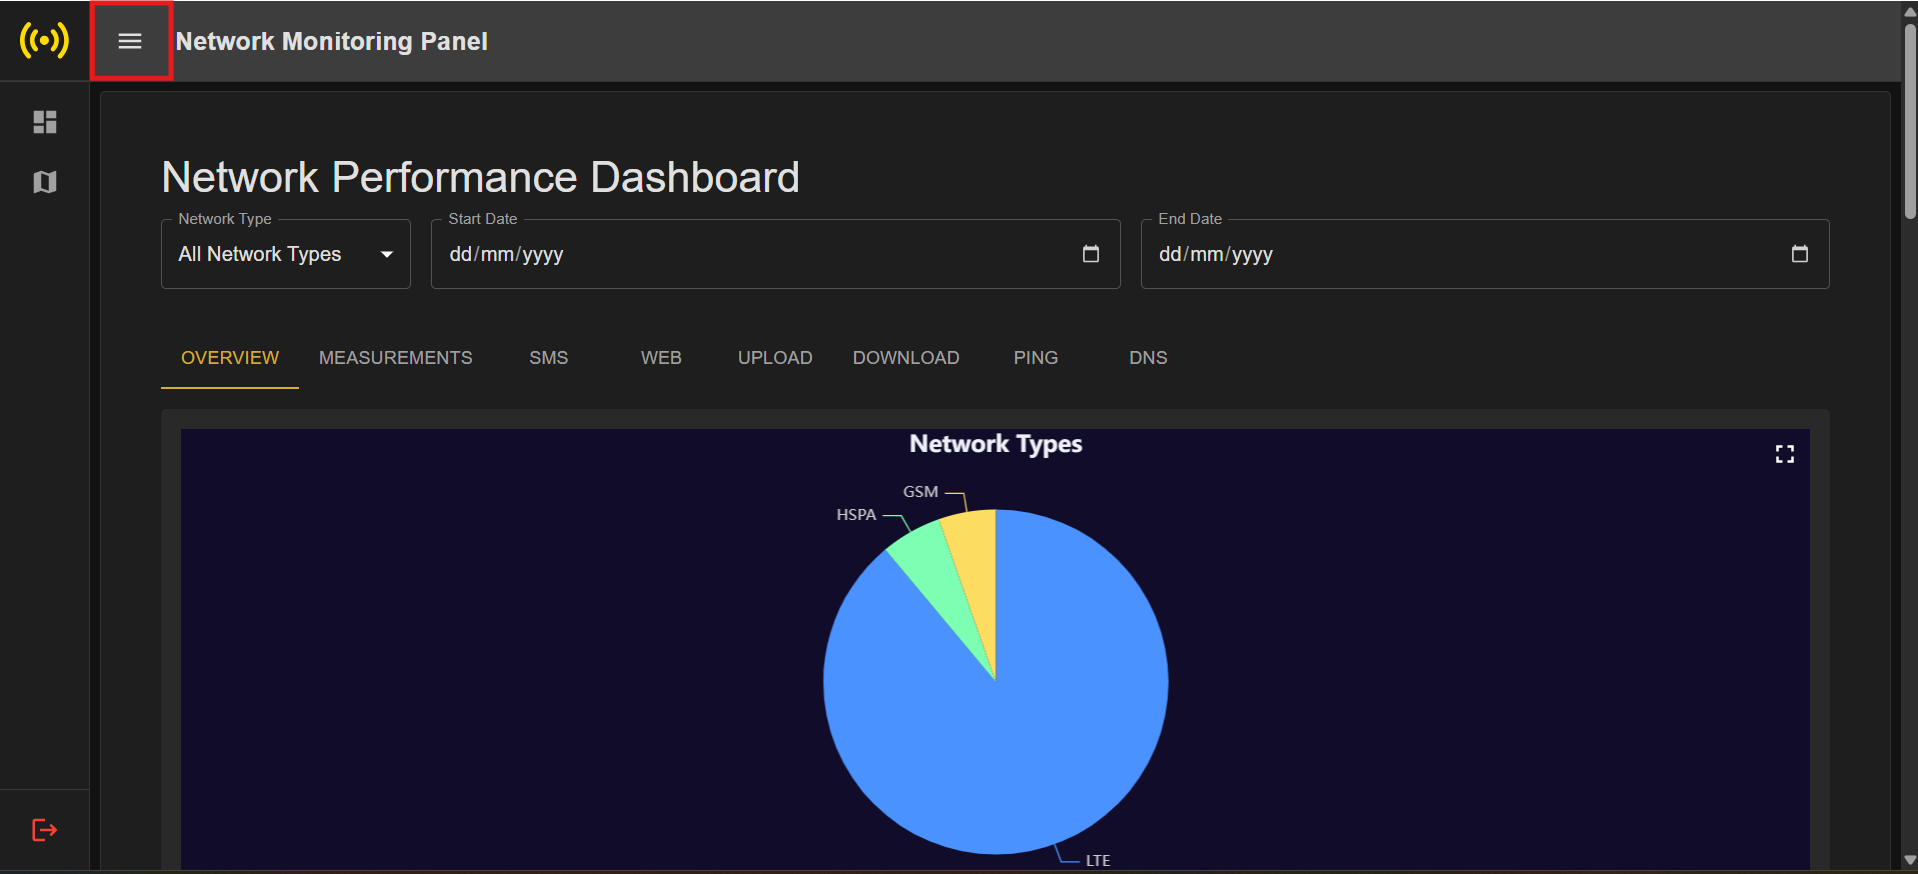
\includegraphics[width=\textwidth]{images/fr-dashboard-without-sidebar.png}
			\end{center}	   		
		در داشبورد وب‌سایت این امکان مقدور گردیده است که داده‌ها بر اساس نوع شبکه پیکربندی شود:
			\begin{center}
				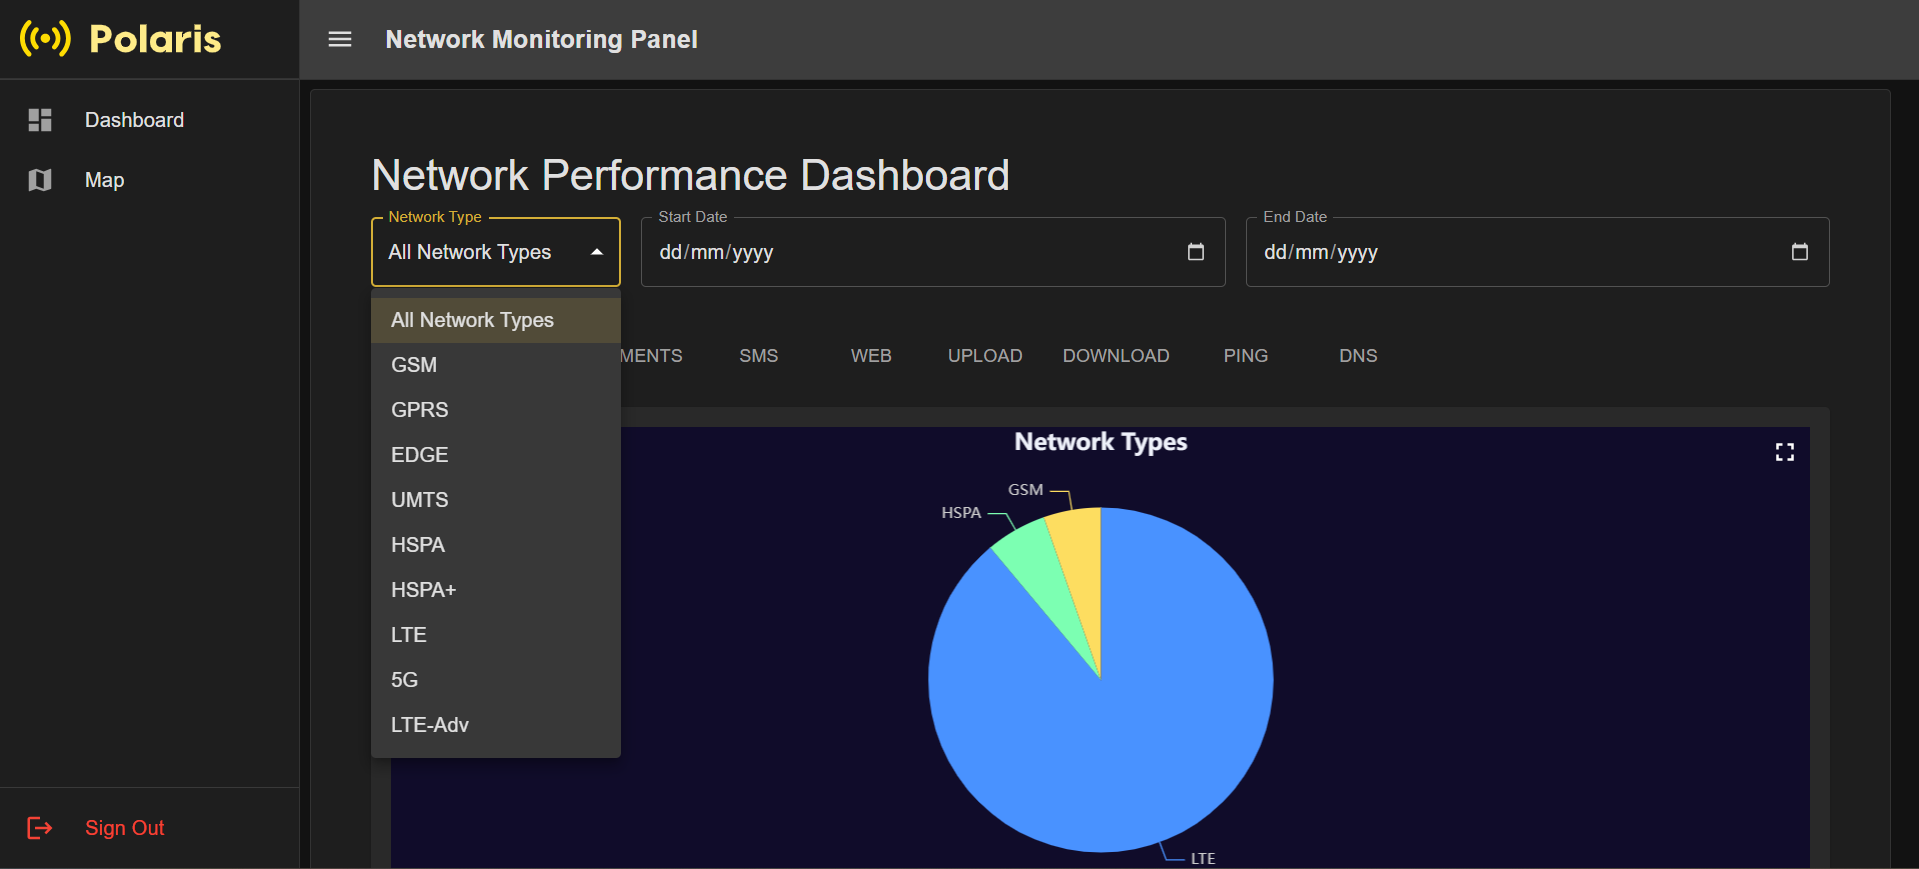
\includegraphics[width=\textwidth]{images/fr-filters-network.png}
			\end{center}	   		
   		در داشبورد وب‌سایت این امکان مقدور گردیده است که داده‌ها بر اساس تاریخ شروع و تاریخ پایان نیز پیکربندی شود:
	   		\begin{center}
	   			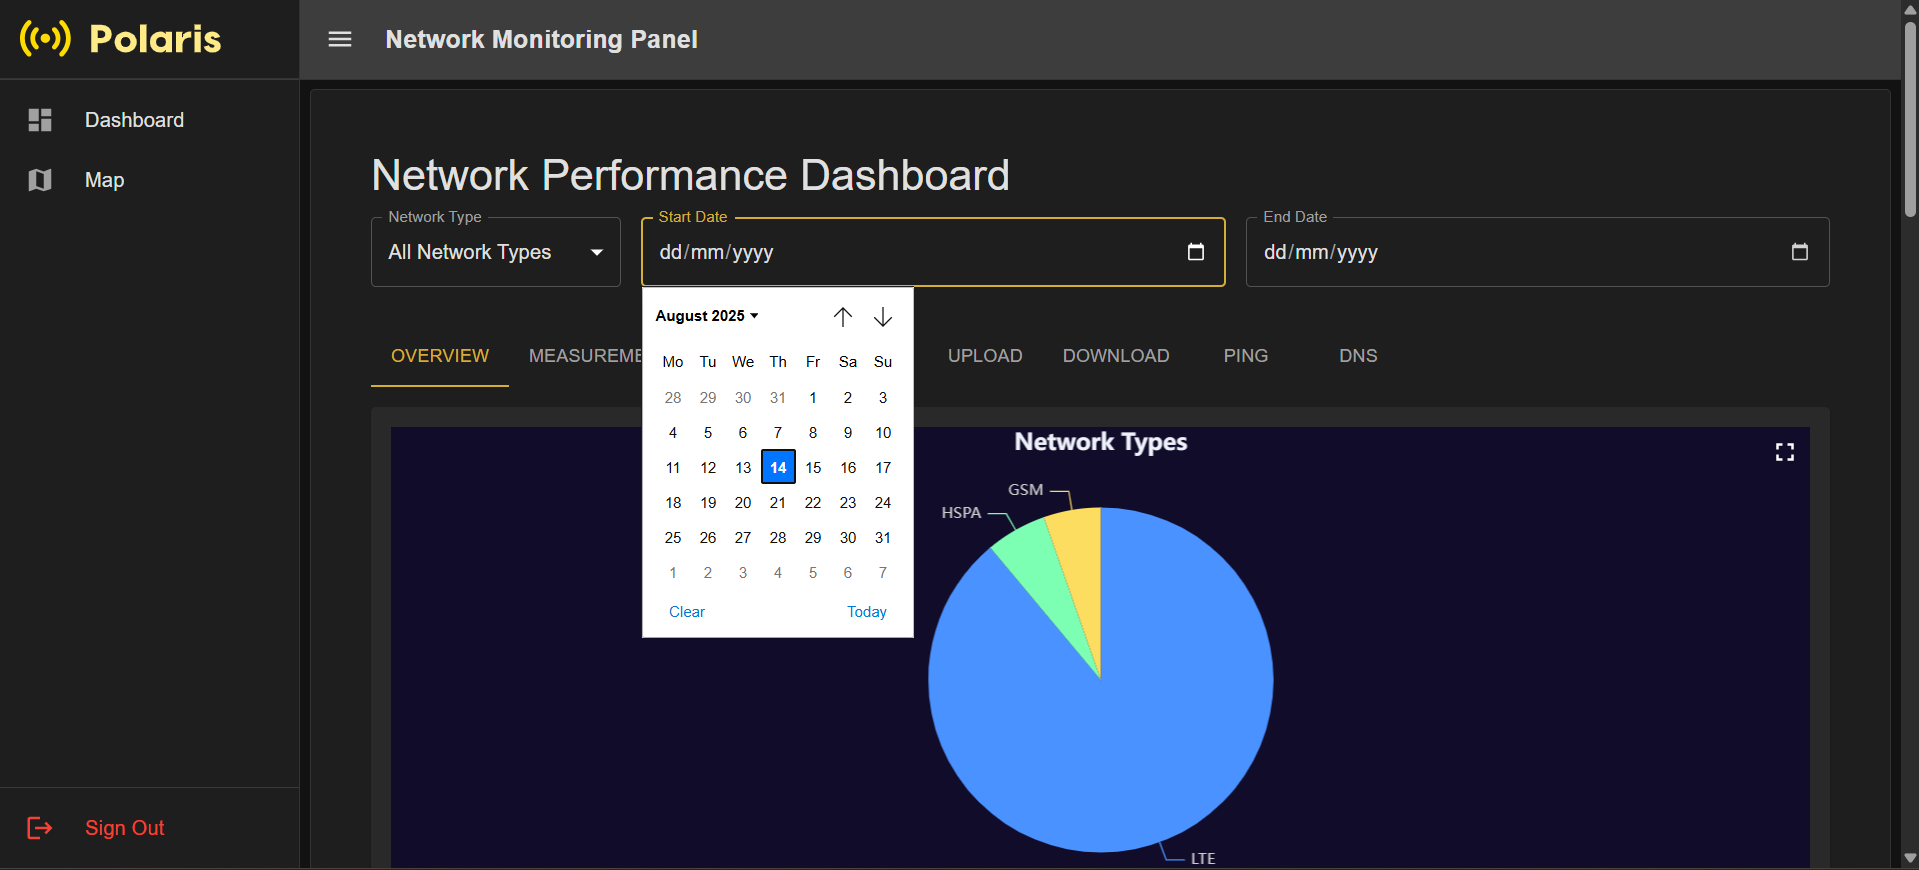
\includegraphics[width=\textwidth]{images/fr-filters-start-date.png}
	   			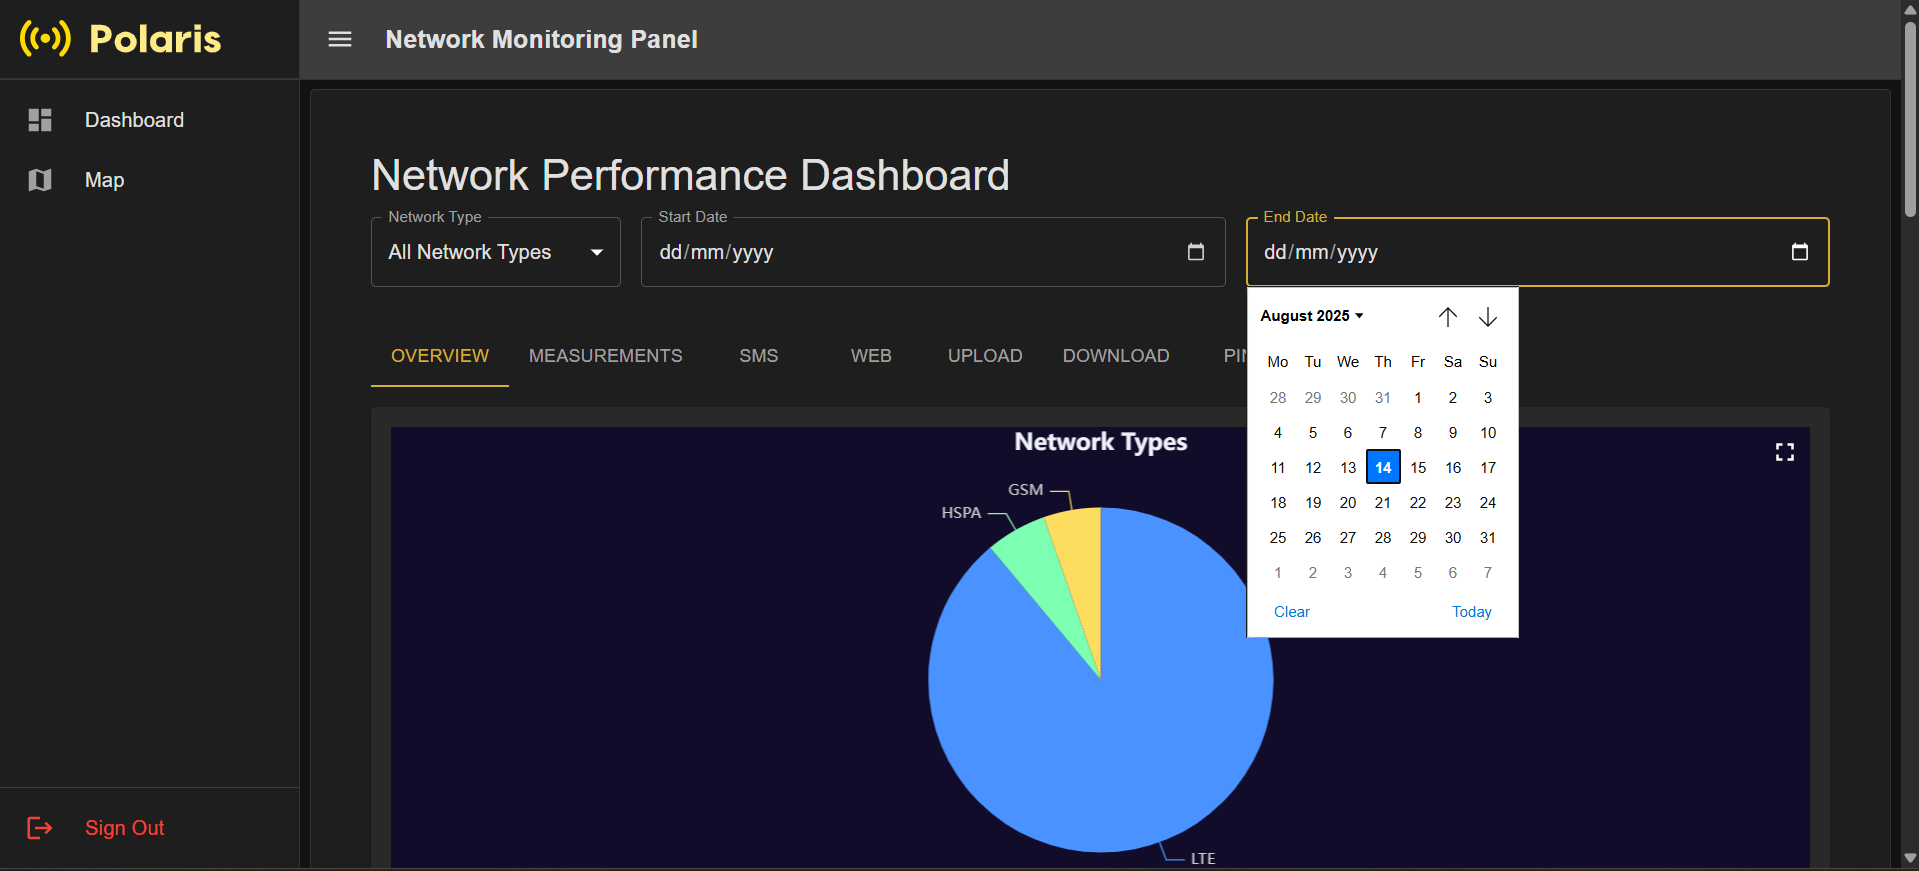
\includegraphics[width=\textwidth]{images/fr-filters-end-date.png}
	   		\end{center}
   		
   		داشبورد در بخش‌های متفاوتی از جمله Overview(که داده‌ها را در یک نگاه نمایش می‌دهد) و Measurements(که اندازه‌گیری‌های غیر از تست‌های تعریف شده توسط کاربر را نمایش می‌دهد) تقسیم شده است و دیگر بخش‌ها مختص تست‌های تعریف شده توسط کاربر است.
   		لازم به ذکر است که هر نمودار دارای دکمه‌ای در گوشۀ بالا سمت راست خود دارد که در تصویر زیر با کادر قرمز رنگ مشخص شده است و این امکان را می‌دهد که نمودار به صورت کامل صفحه را می‌پوشاند و باعث مشاهده بهتر آن می‌شود:
	   		\begin{center}
	   			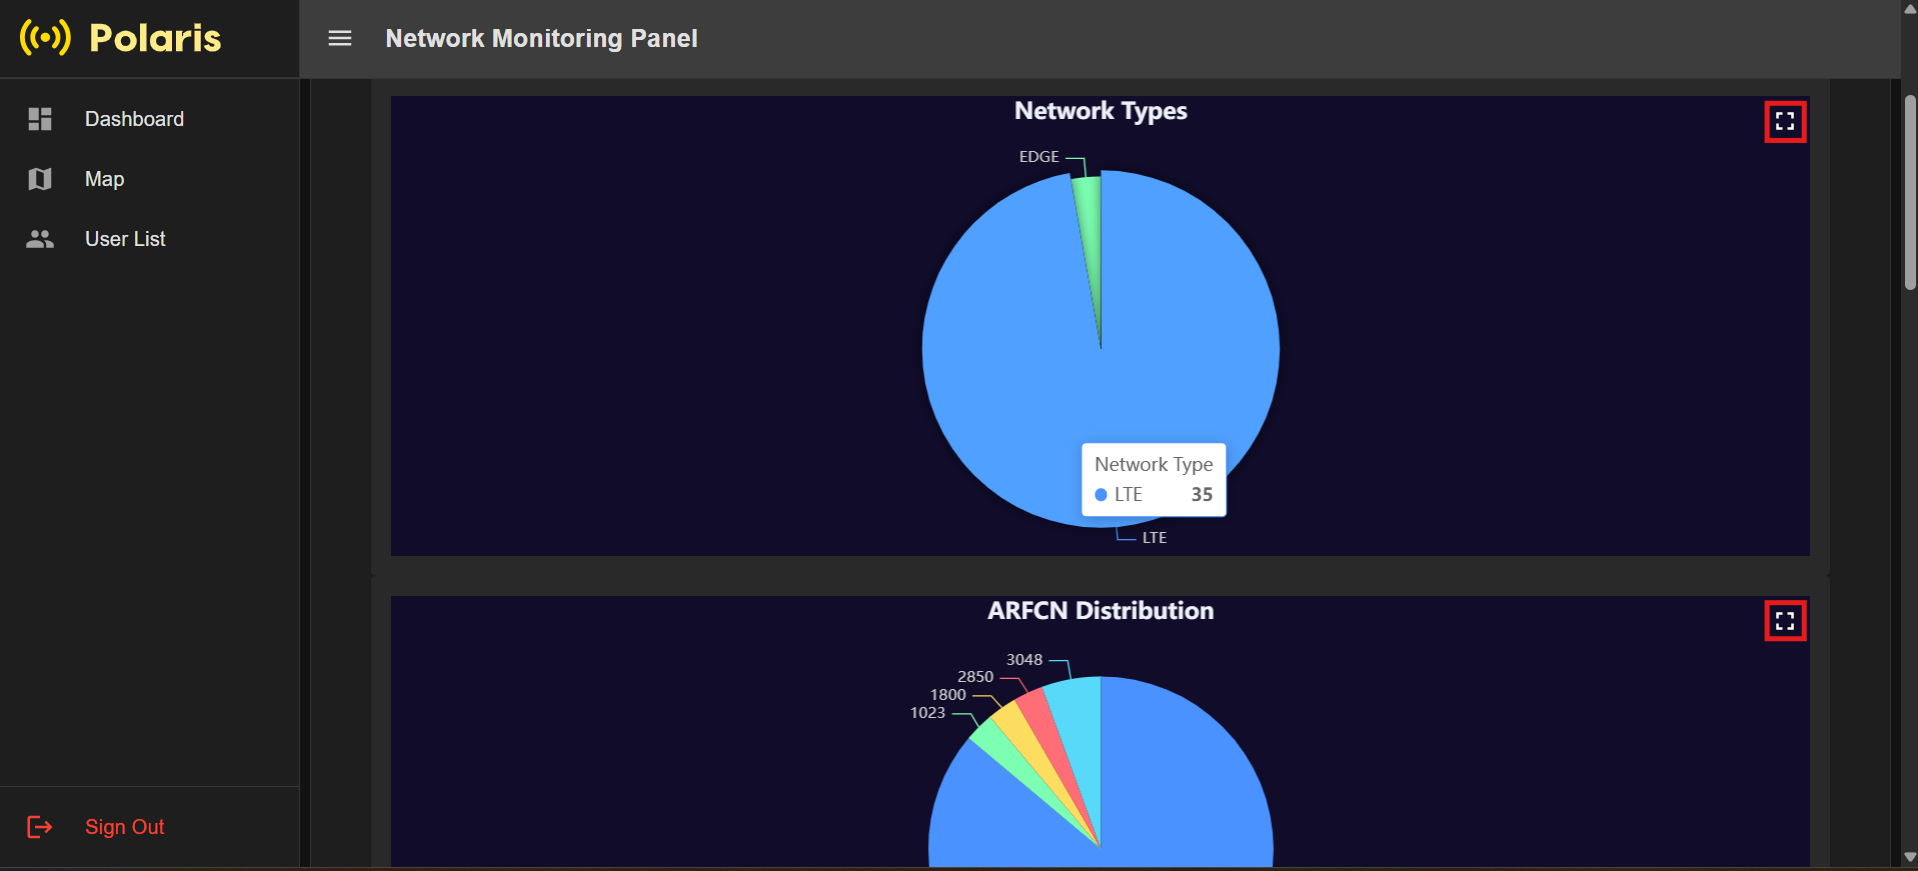
\includegraphics[width=\textwidth]{images/fr-chart-minimize.png}
	   		\end{center}
   		در این حالت با زدن روی این دکمه صفحه به صورت زیر خواهد شد که با انتخاب دکمه ضربدر که با کادر قرمز رنگ مشخص شده است صفحه به حالت قبلی بر‌میگردد:
	   		\begin{center}
				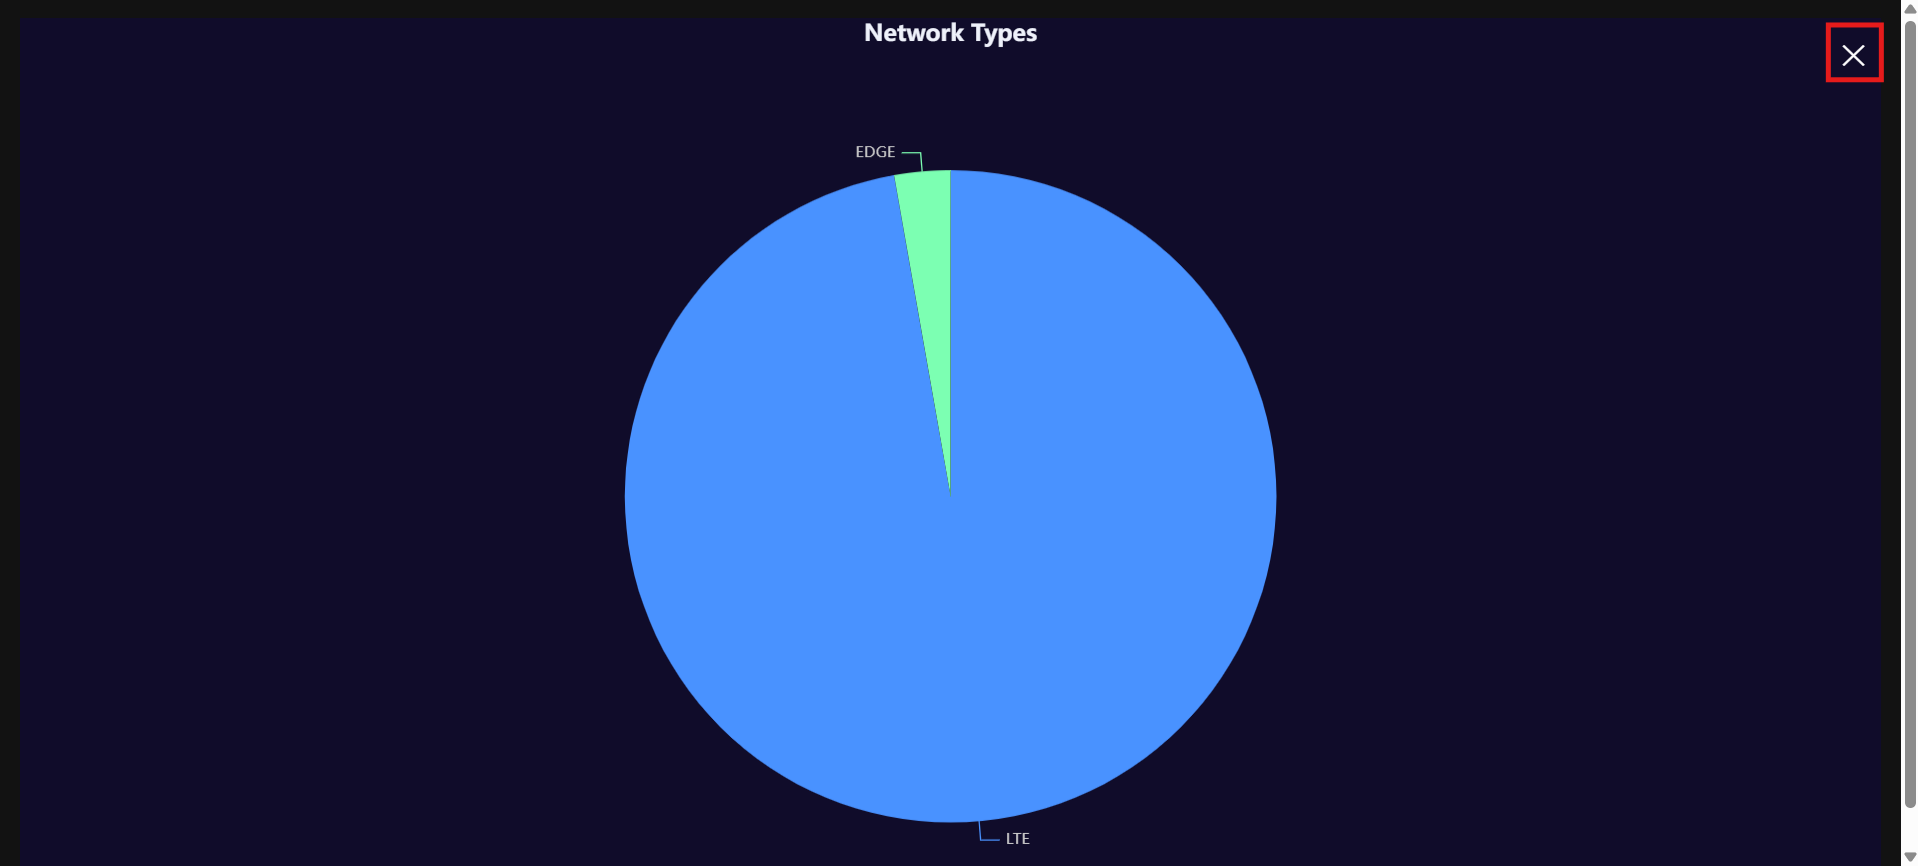
\includegraphics[width=\textwidth]{images/fr-chart-maximize.png}
			\end{center}
		در انتهای هر بخش داشبورد یک جدول وجود دارد که امکان مشاهده همه اطلاعات را در یک نگاه می‌دهد. همجنین قابلیت استخراج اطلاعات به صورت csv و kml نیز آمده است که با کلیک روی دکمه آن(که با کادر قرمز رنگ مشخص شده است) فایل با فرمت موردنظر دانلود می‌شود:
			\begin{center}
				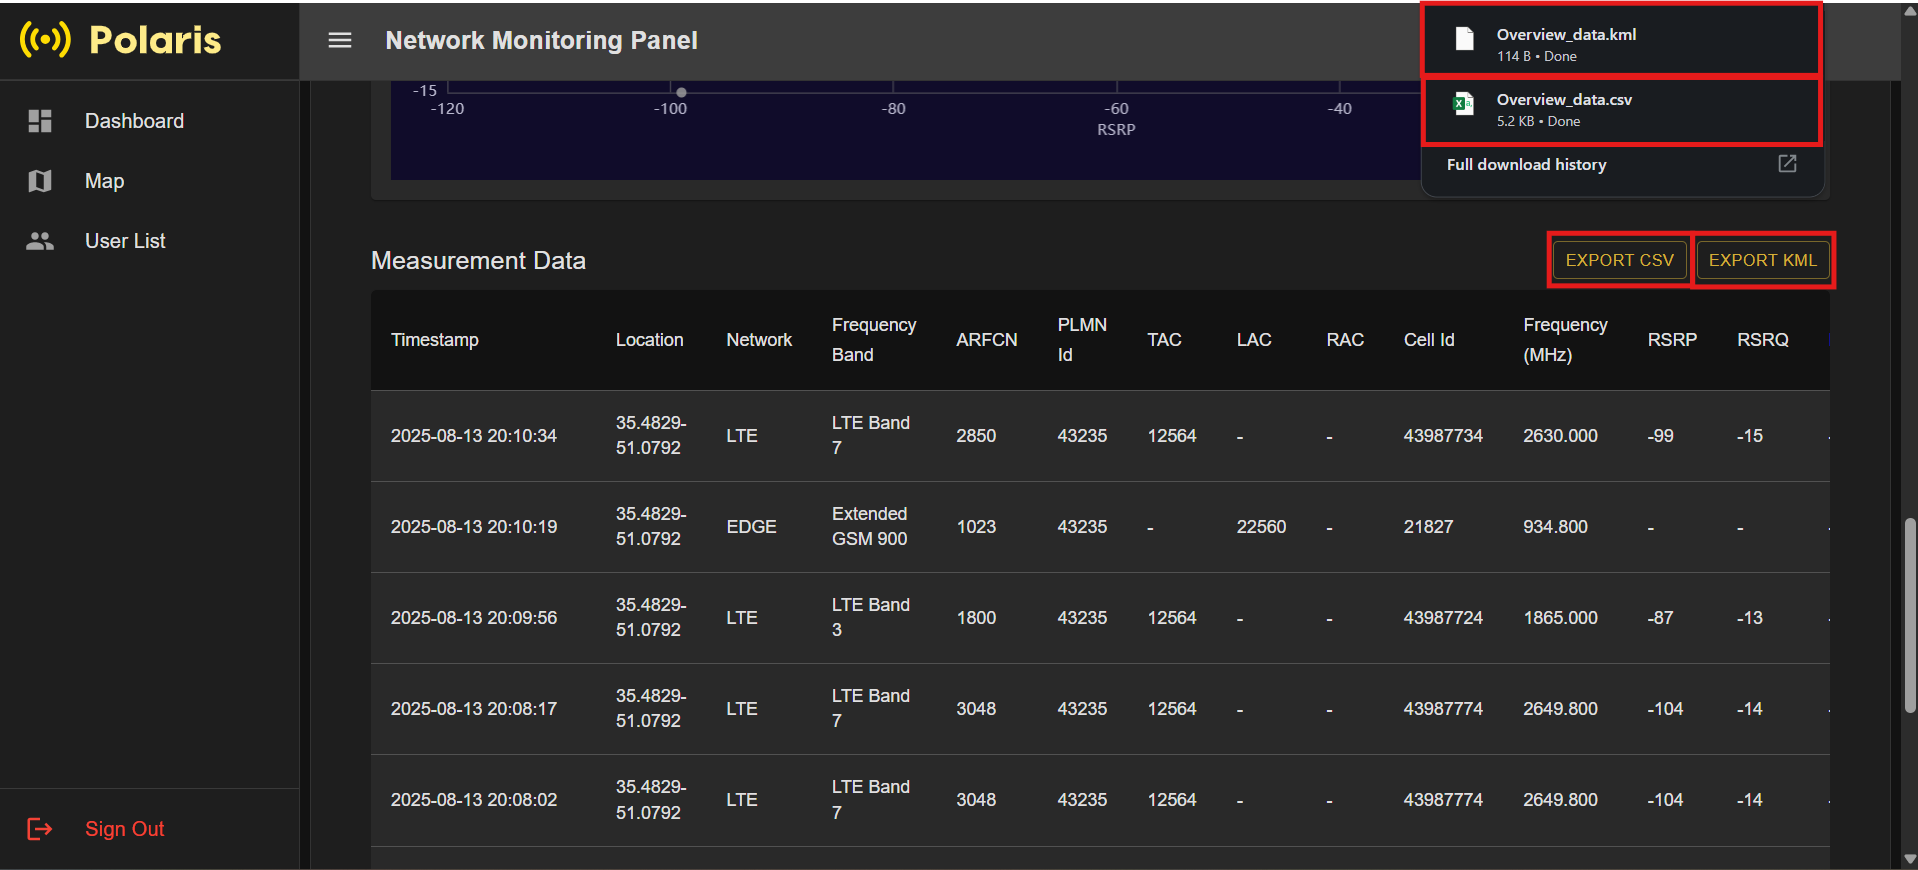
\includegraphics[width=\textwidth]{images/fr-table-export.png}
			\end{center}
   		از آنجایی که احتمالا هر کاربر تعداد زیادی داده خواهد داشت هر جدول تعداد محدودی از داده‌ها را نمایش می‌دهد که می‌توان آن را تغییر داد. همچنین می‌توان بین داده‌های هر صفحه جابه‌جا شد و انتهای جدول نمایش می‌دهد که این اطلاعات کدامین ردیف‌های اطلاعات کاربر می‌باشند و کاربر چه تعداد اطلاعات دارد:
   			\begin{center}
   				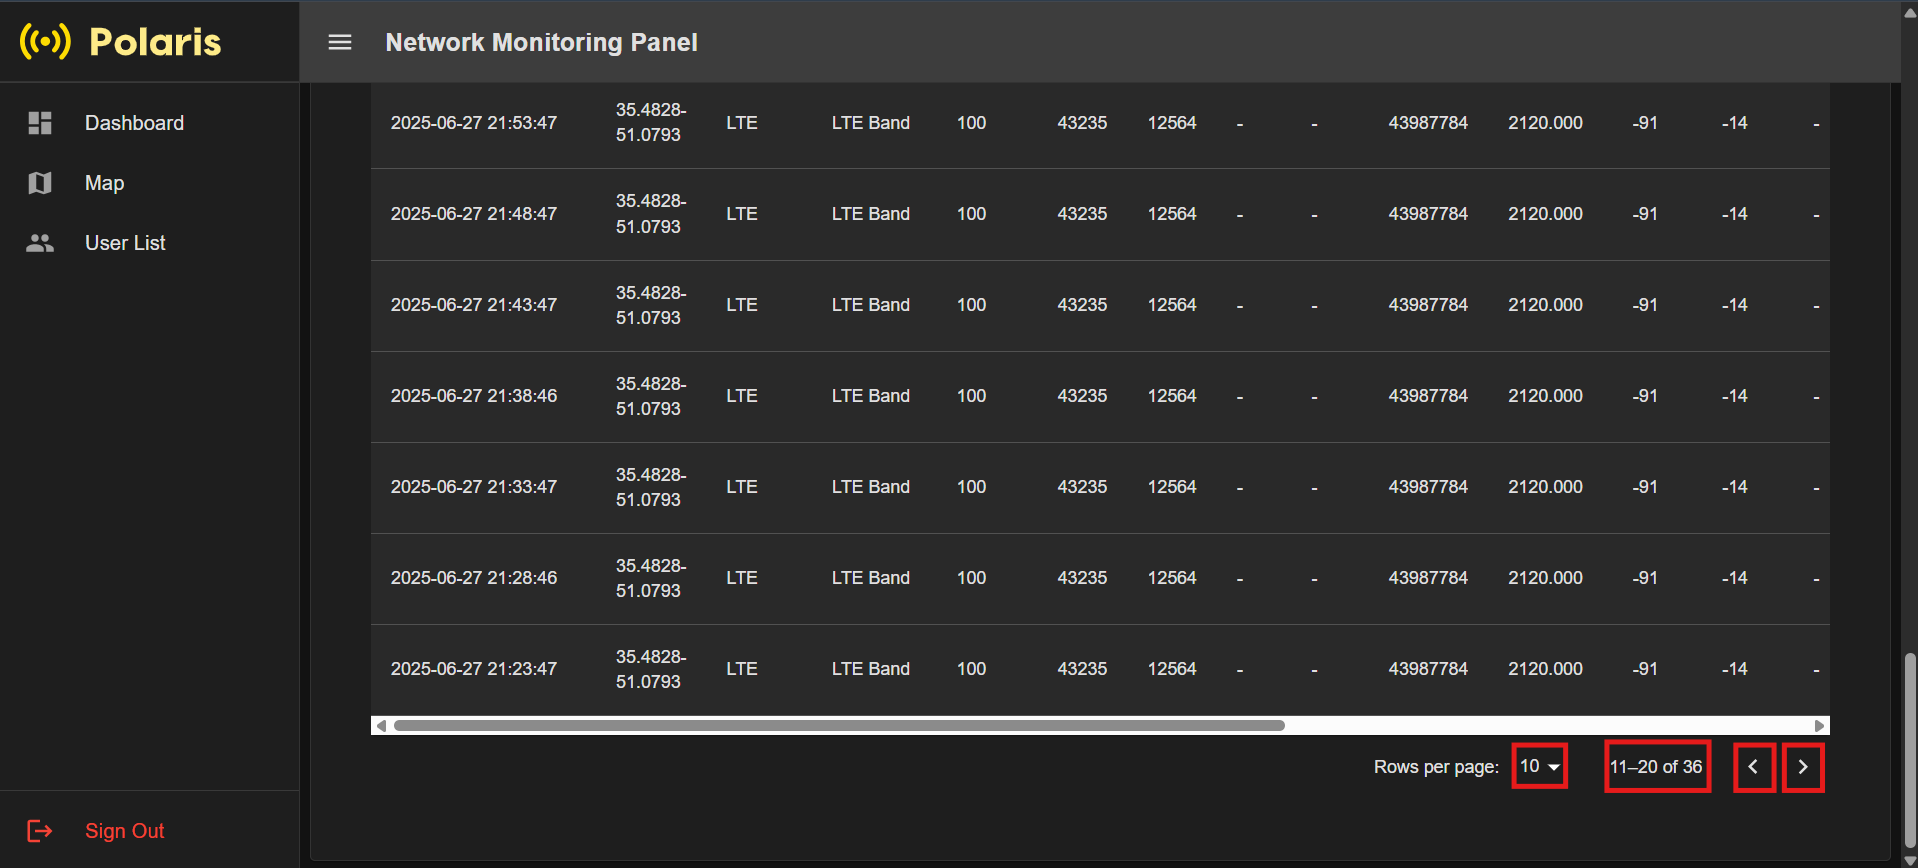
\includegraphics[width=\textwidth]{images/fr-table-pagination.png}
   			\end{center}
    	\item  استفاده از نقشه: توضیح نحوه تعامل با ویژگی نقشه.
    	\item  خروج از سیستم: می‌توان از طریق کلیک بر روی دکمه \lr{Sign Out} که در تصویر زیر نیز مشخص شده است از حساب کاربری خود خروج پیدا کرد:
    		\begin{center}
    			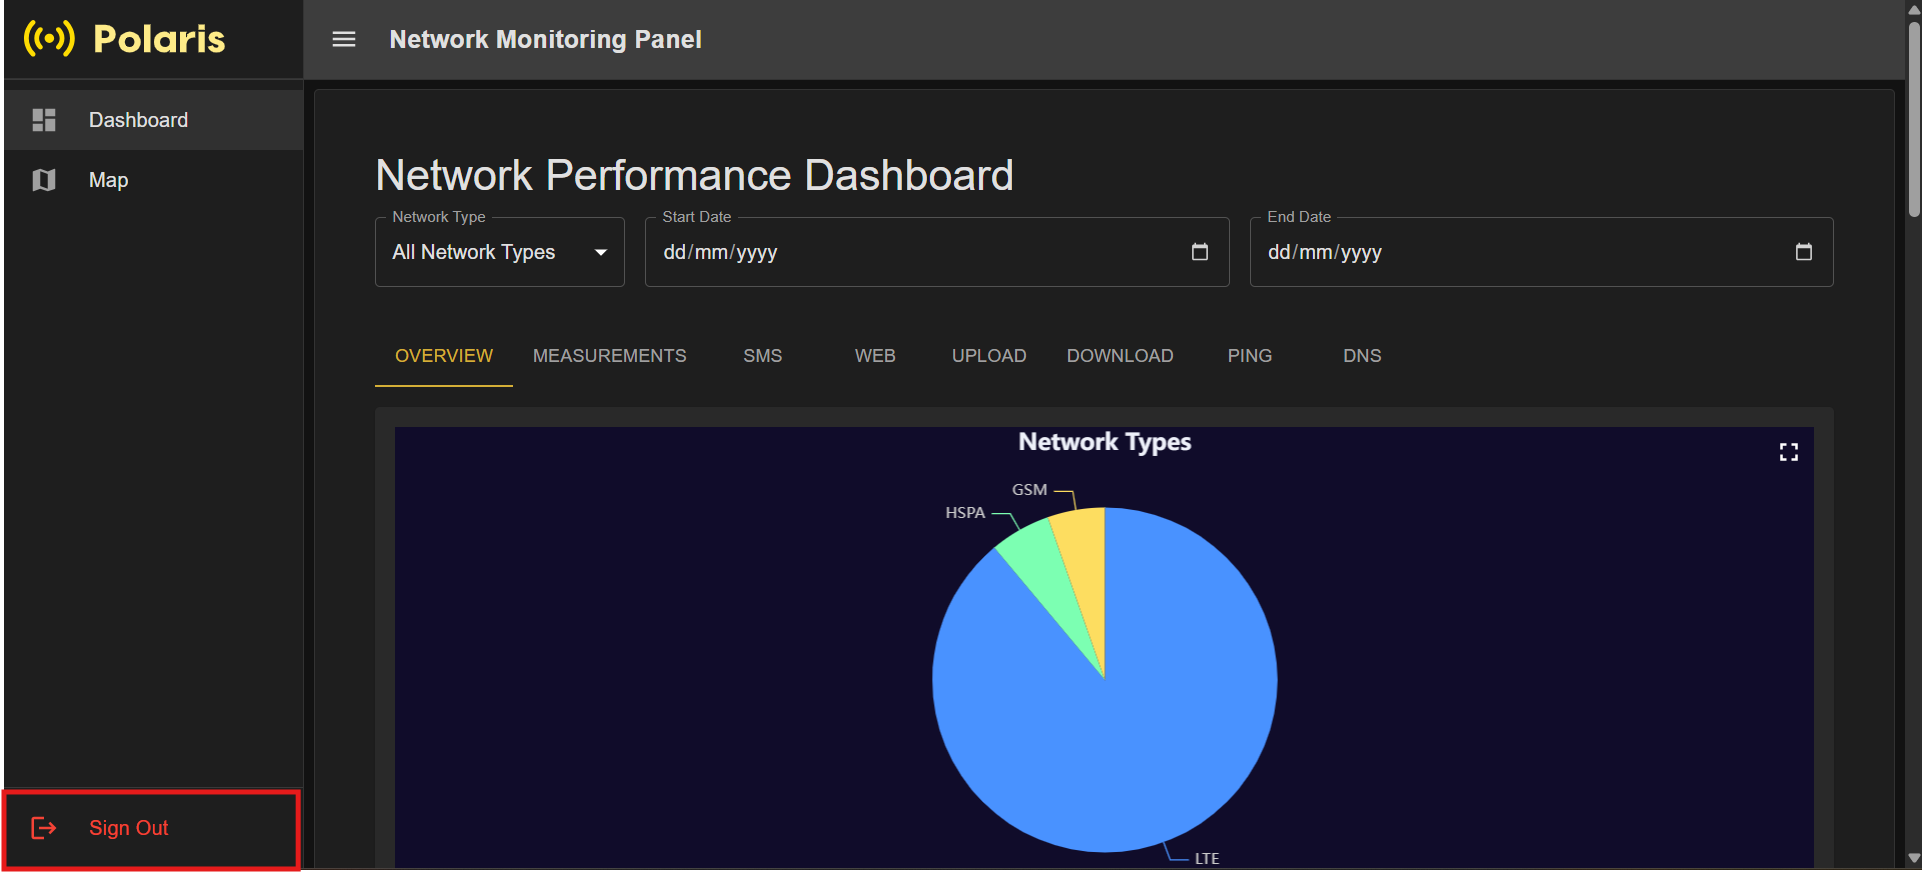
\includegraphics[width=\textwidth]{images/fr-signout.png}
    		\end{center}
    \end{itemize}
    \section{ویژگی‌های مدیر}
    \begin{itemize}
    	\item  لیست کاربران: فردی که توسط سرور به عنوان ادمین انتخاب شود می‌تواند لیست همه کاربران غیر ادمین به همراه اطلاعات آن ها را مشاهده کند که به صورت زیر است:
    		\begin{center}
    			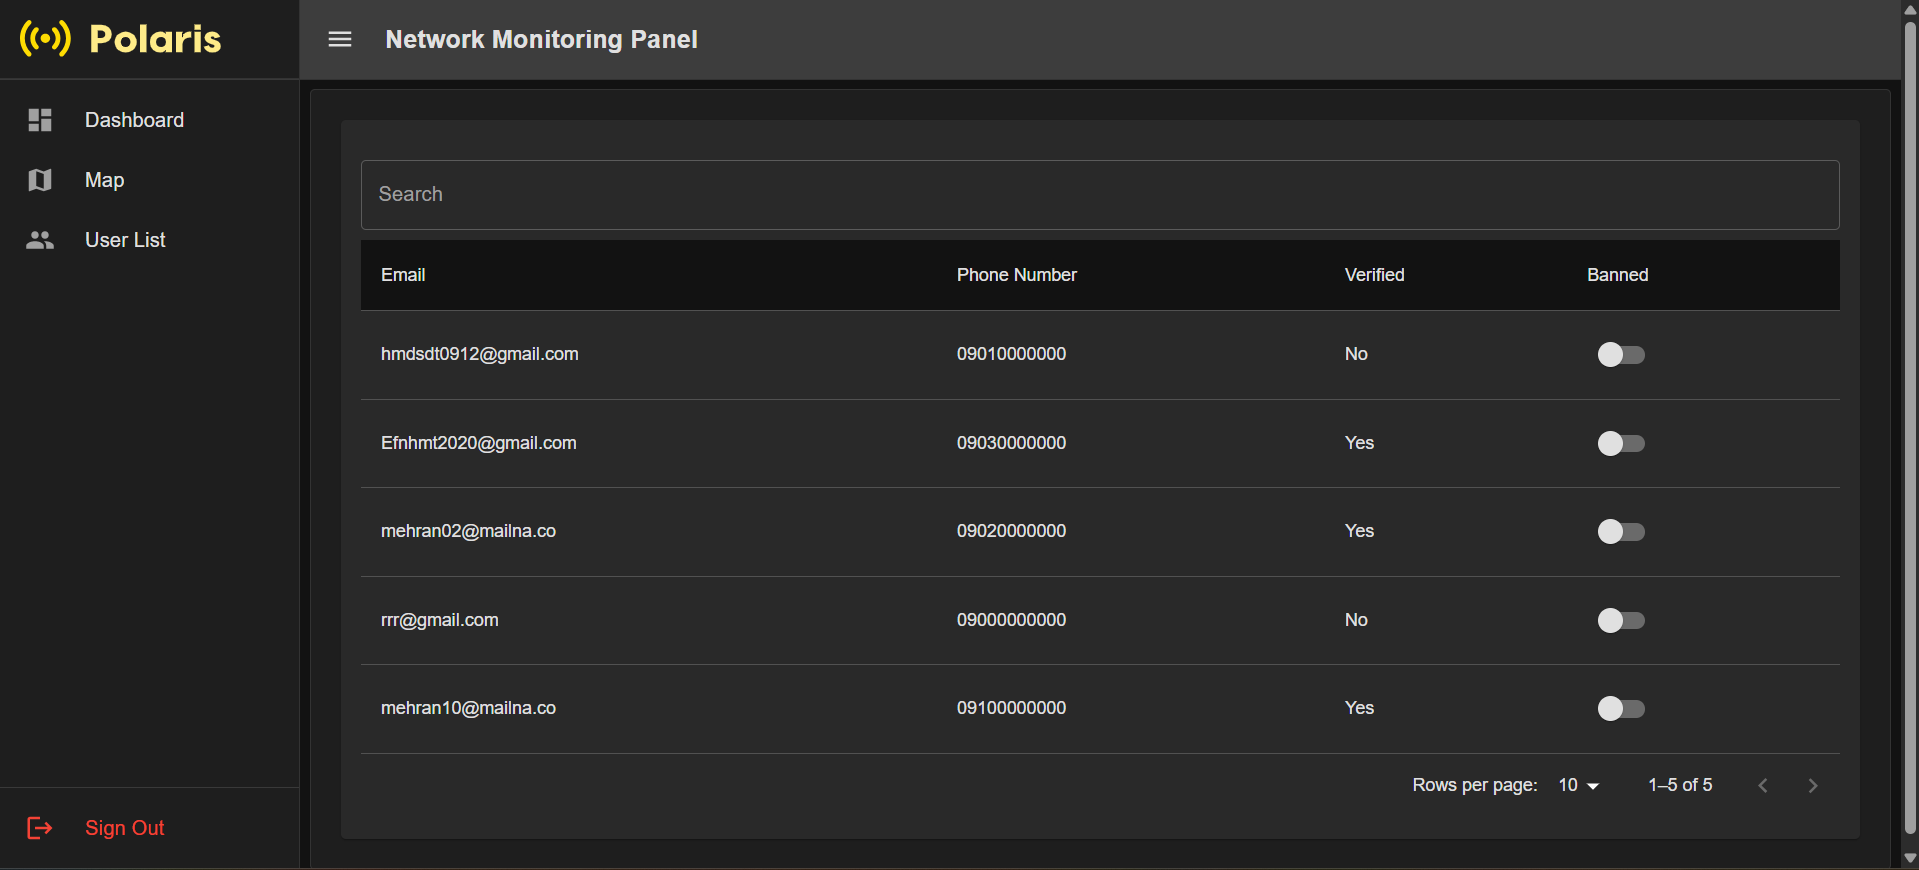
\includegraphics[width=\textwidth]{images/fr-userlist.png}
    		\end{center}
    	این امکان به مدیر داده شده است که بتواند یک کاربر را به حالت تعلیق در بیاورد به این صورت که در ستون Banned می‌تواند سوییچ را روشن و خاموش کند که در صورت روشن کردن کاربر موردنظر دیگر امکان ورود به حساب خود را ندارد و در صورت خاموش بودن روند ورود کاربر به حساب خود به صورت عادی خواهد بود:
    		\begin{center}
    			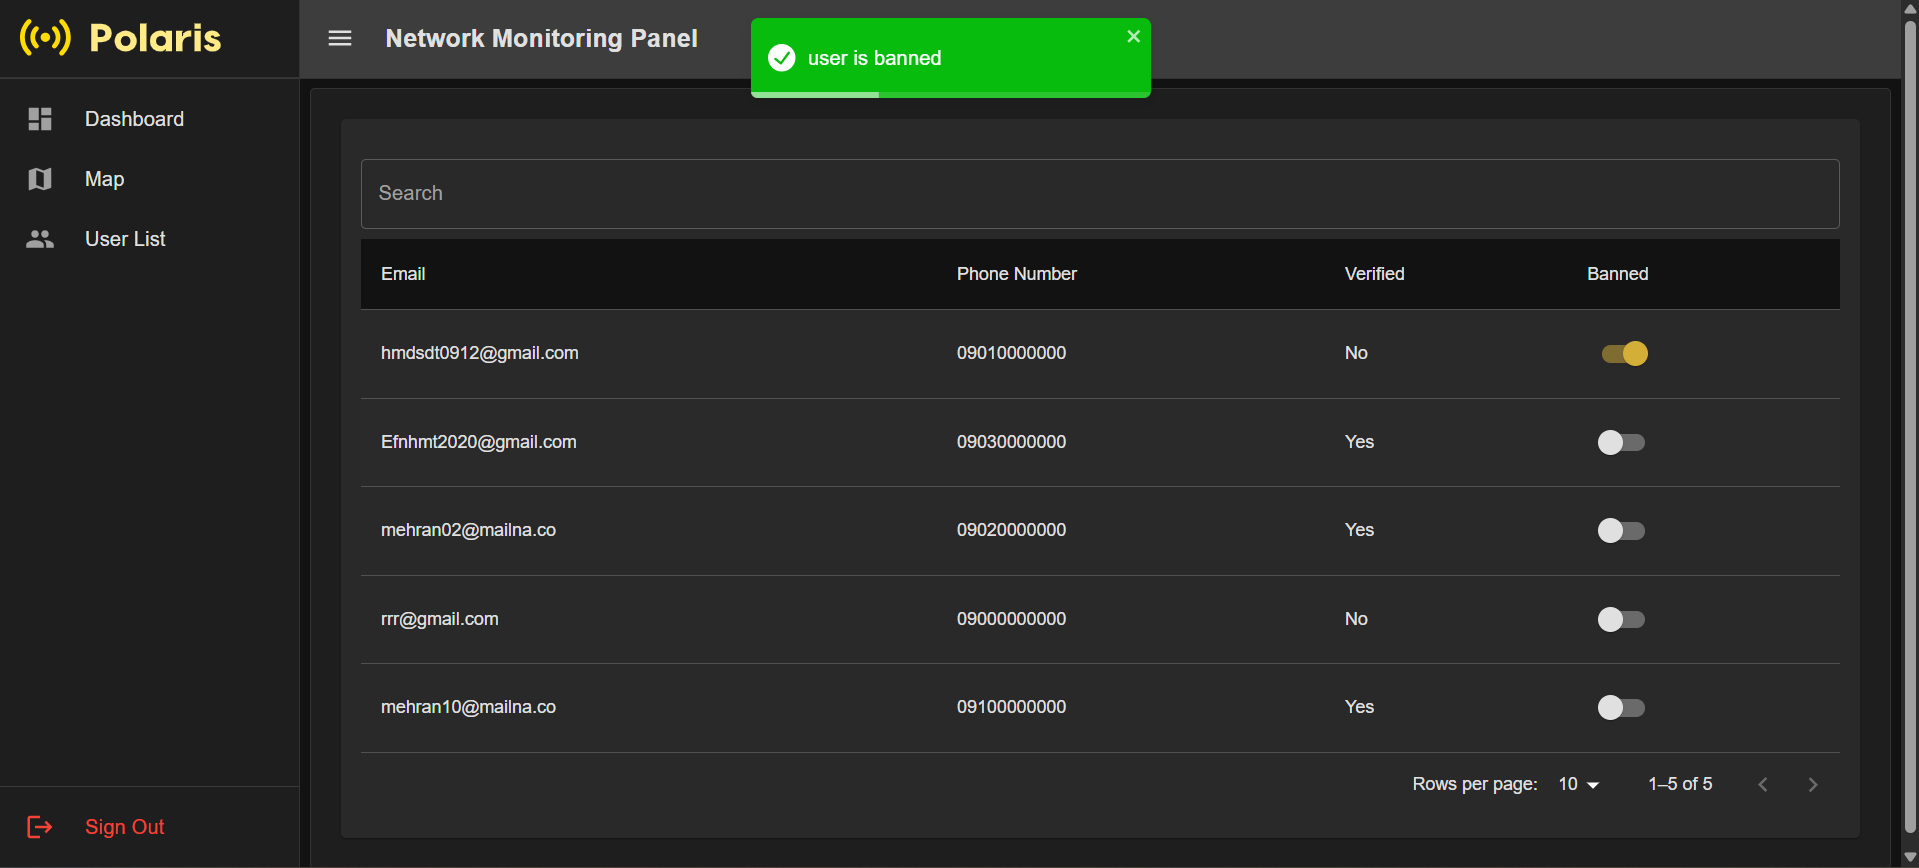
\includegraphics[width=\textwidth]{images/fr-userlist-ban.png}
    			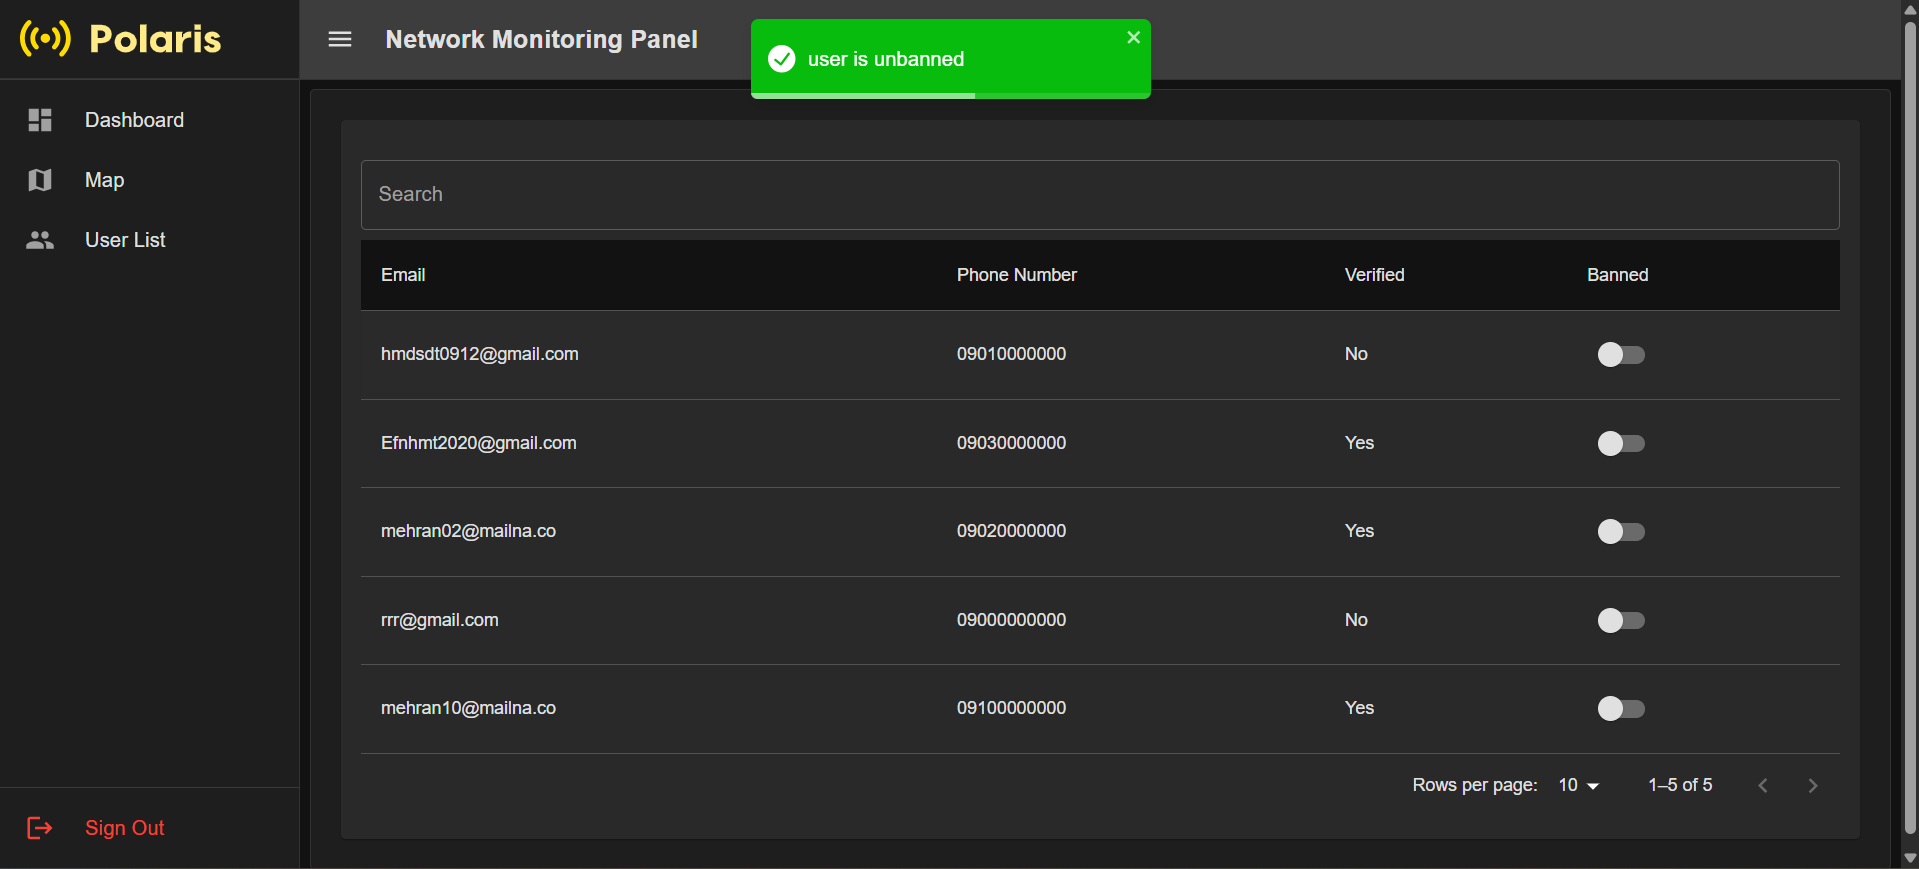
\includegraphics[width=\textwidth]{images/fr-userlist-unban.png}
    		\end{center}
   		همچنین این قابلیت برای مدیر ایجاد شده است که در نوار Search در بین پست الکترونیک کاربران و یا شماره همراه آن‌ها جست و جو کند. برای مثال در تصویر زیر واژه hmd جست و جو شده است و تنها یک نتیجه نمایش داده شده است:
   		\begin{center}
   			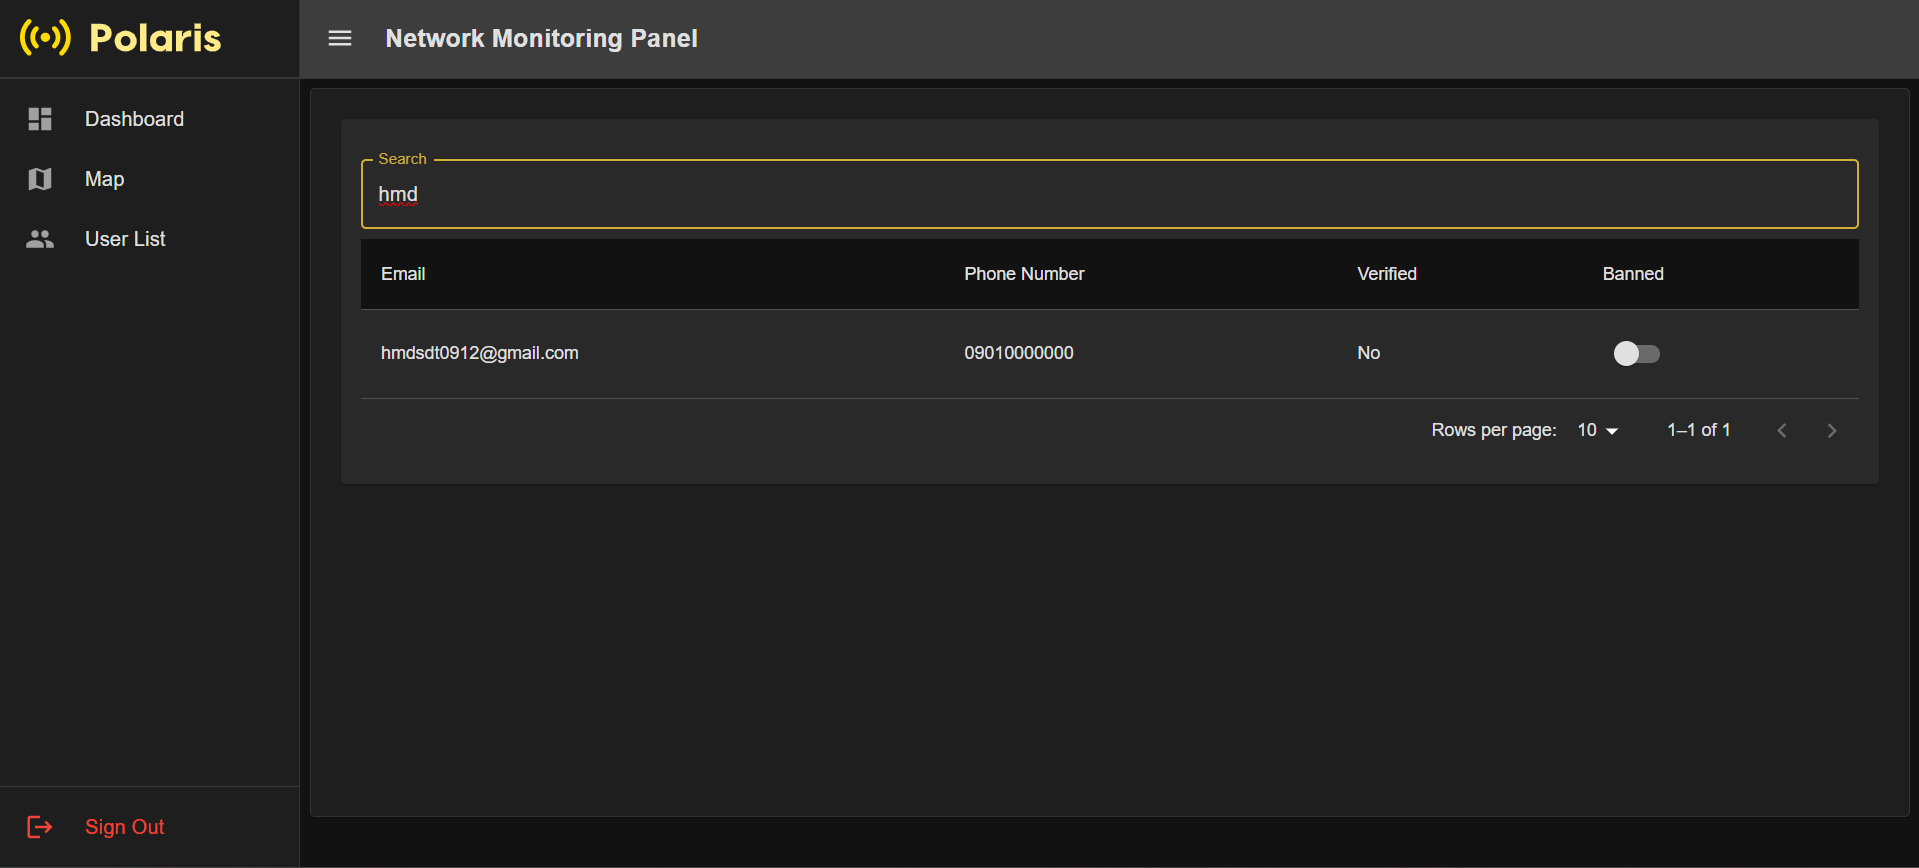
\includegraphics[width=\textwidth]{images/fr-userlist-search.png}
   		\end{center}
   		
    \end{itemize}

    \section{نقشه}
\begin{itemize}
    \item برای ورود به صفحه‌ی نقشه، کافی است گزینه‌ی \textbf{«نقشه»} در بالای سمت چپ صفحه را انتخاب کنید.
    \begin{center}
        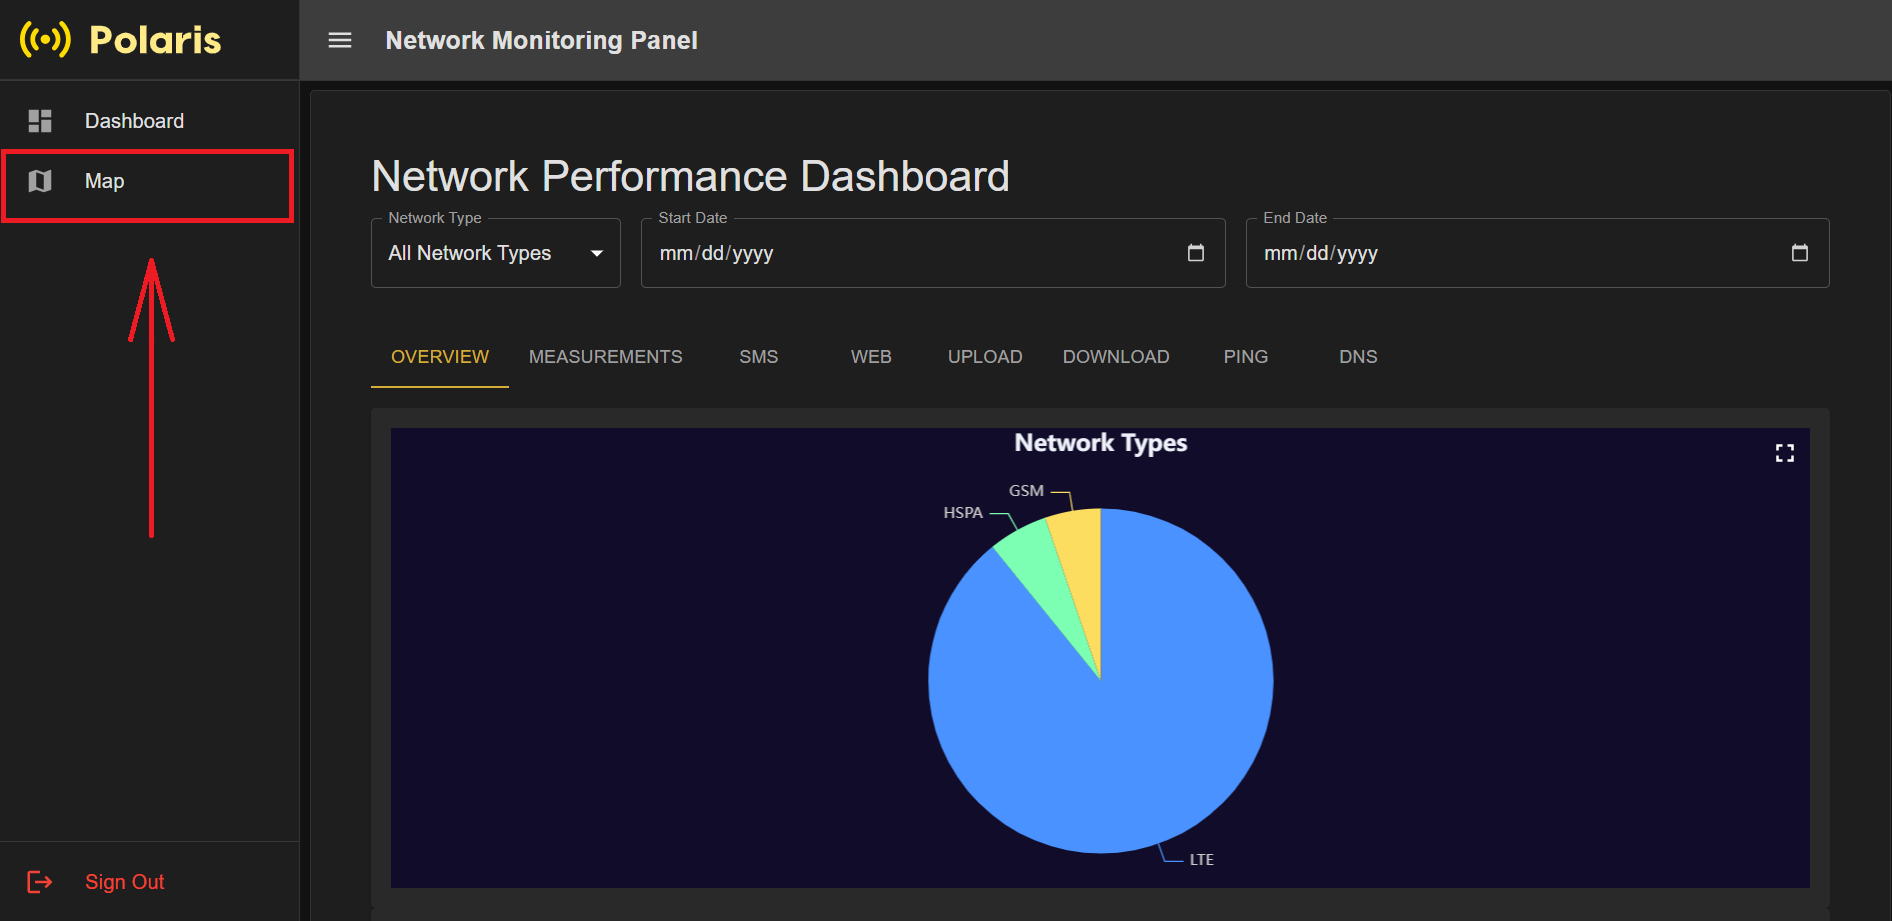
\includegraphics[width=\textwidth]{images/go_to_map.png}
    \end{center}

    \item پس از ورود، صفحه‌ی زیر نمایش داده خواهد شد:
    \begin{center}
        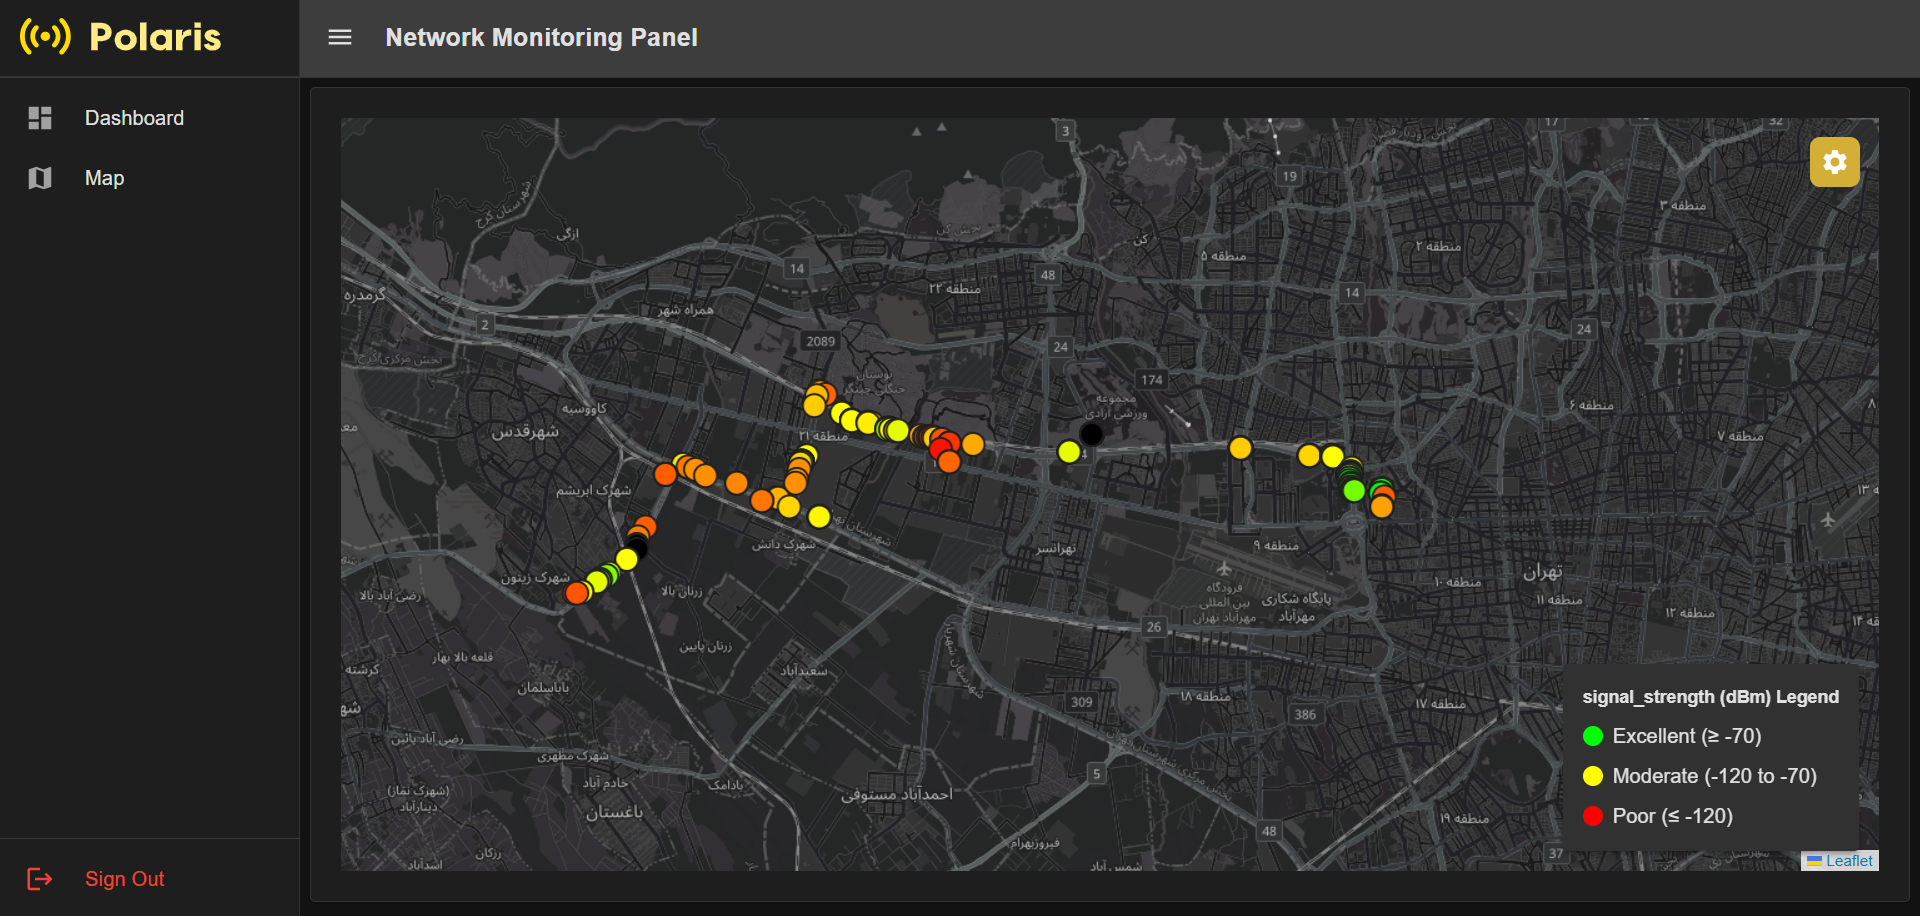
\includegraphics[width=\textwidth]{images/map_overall.png}
    \end{center}

    \item در تصویر زیر، قابلیت‌ها و دکمه‌های این صفحه توضیح داده شده‌اند:
    \begin{center}
        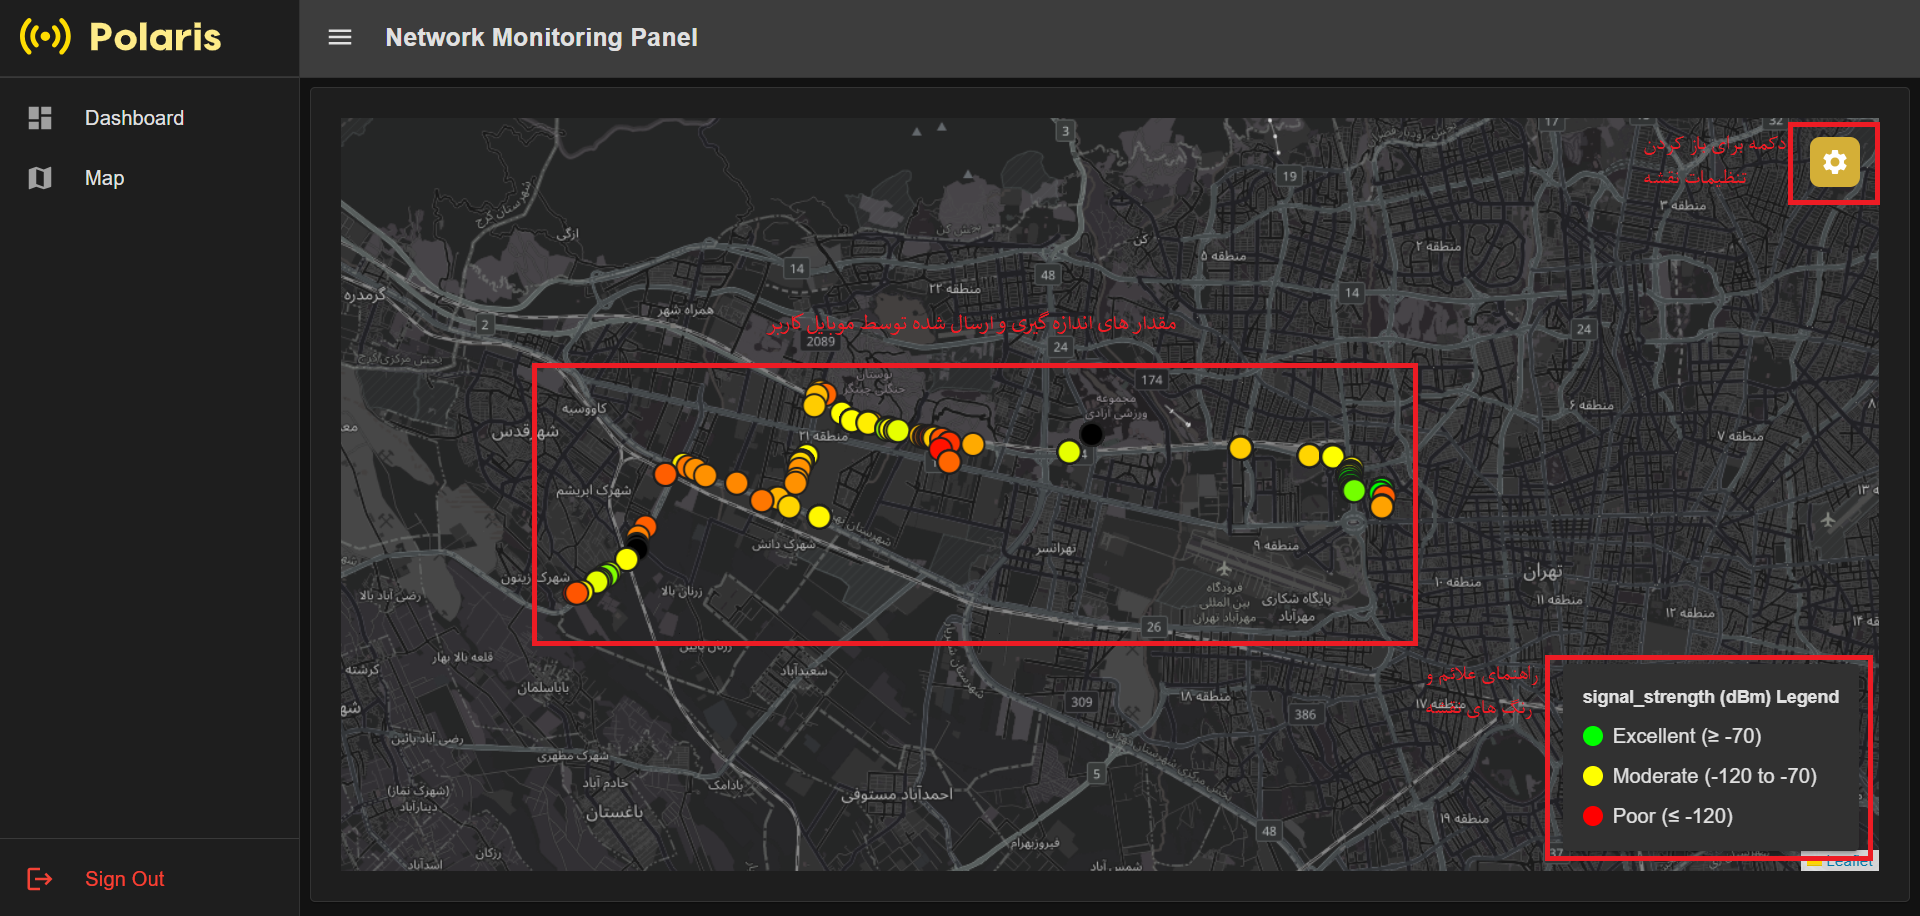
\includegraphics[width=\textwidth]{images/map_overall_explained.png}
    \end{center}

    \item اندازه‌گیری‌های ارسال‌شده توسط کاربران، بر اساس کیفیت آنها با رنگ نمایش داده می‌شوند.\\
    به‌عنوان مثال، اگر رنگ قرمز نشان‌دهنده‌ی کیفیت پایین و رنگ سبز نشان‌دهنده‌ی کیفیت بالا باشد، هر گزارش با طیفی بین این دو رنگ نمایش داده خواهد شد.\\
    در بخش راهنمای نقشه، معیارهای رنگ برای هر \lr{metric} نمایش داده شده‌اند.\\
    \textbf{نکته:} اگر داده‌ی مربوط به یک گزارش موجود نباشد، رنگ آن به صورت مشکی نمایش داده می‌شود.

    \item برای مشاهده‌ی جزئیات یک گزارش، کافی است آن را انتخاب کنید تا اطلاعات کامل آن نمایش داده شود:
    \begin{center}
        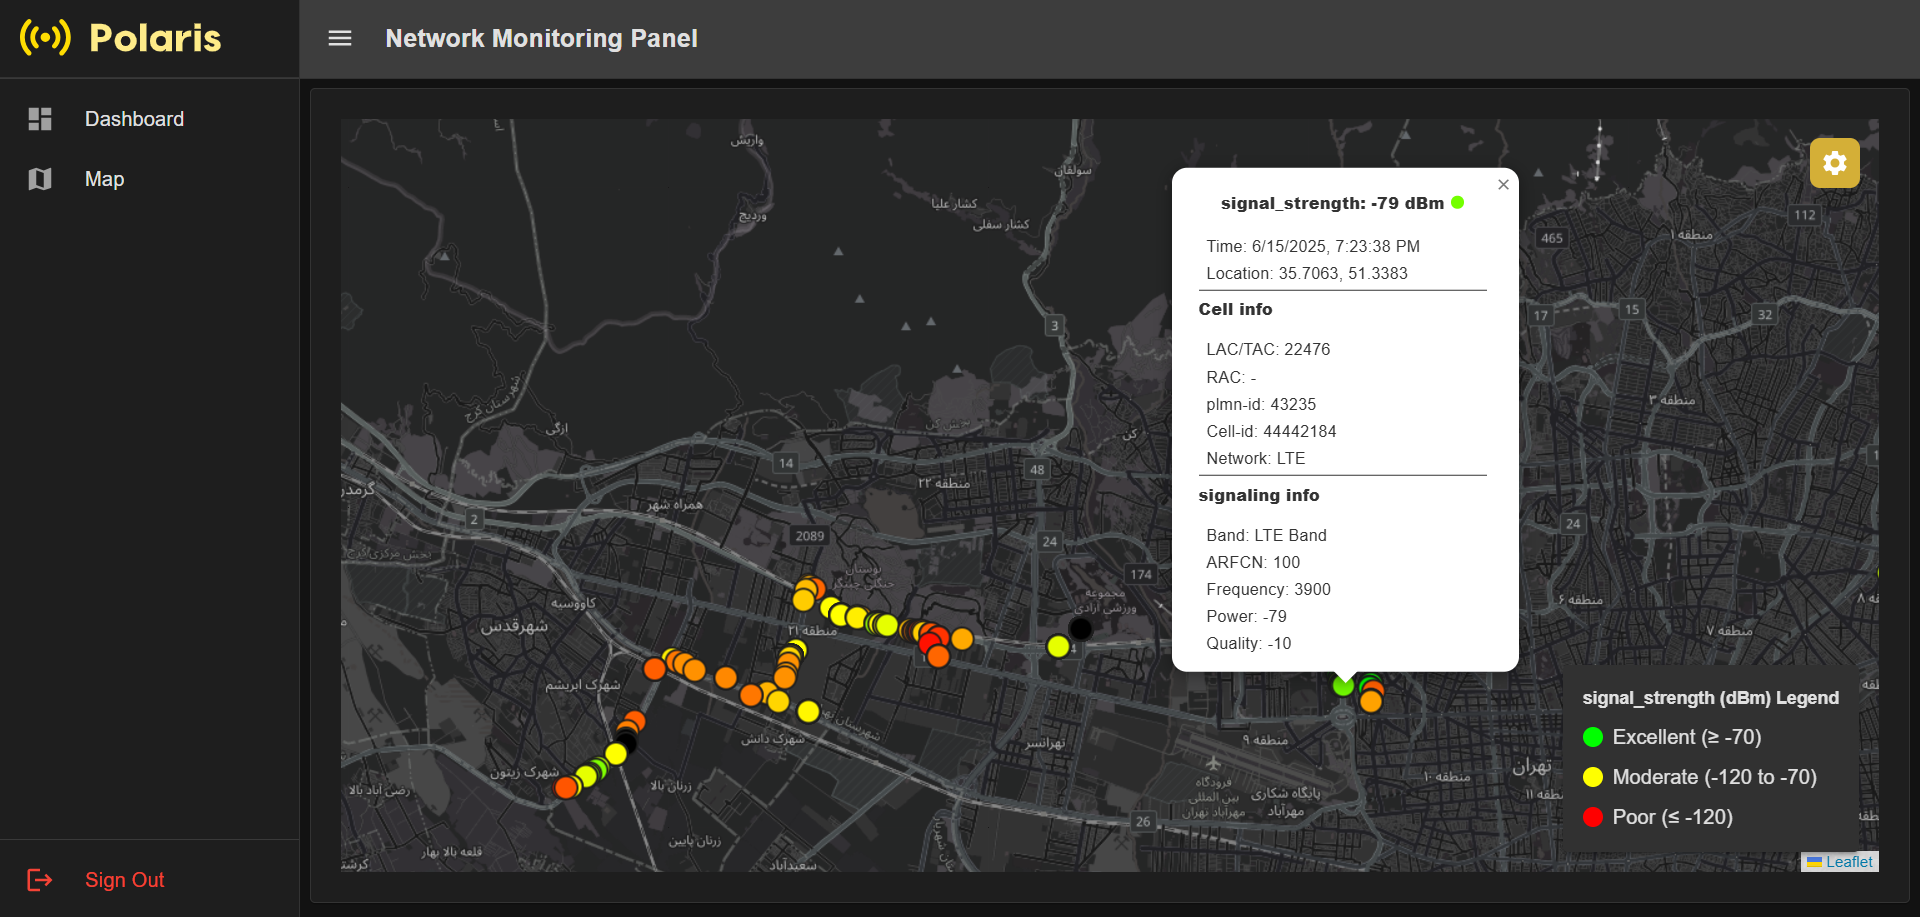
\includegraphics[width=\textwidth]{images/map_popup_open.png}
    \end{center}

    \item برای تغییر تنظیمات، دکمه‌ی \textbf{«تنظیمات»} را انتخاب کنید. سپس صفحه‌ی زیر نمایش داده می‌شود:
    \begin{center}
        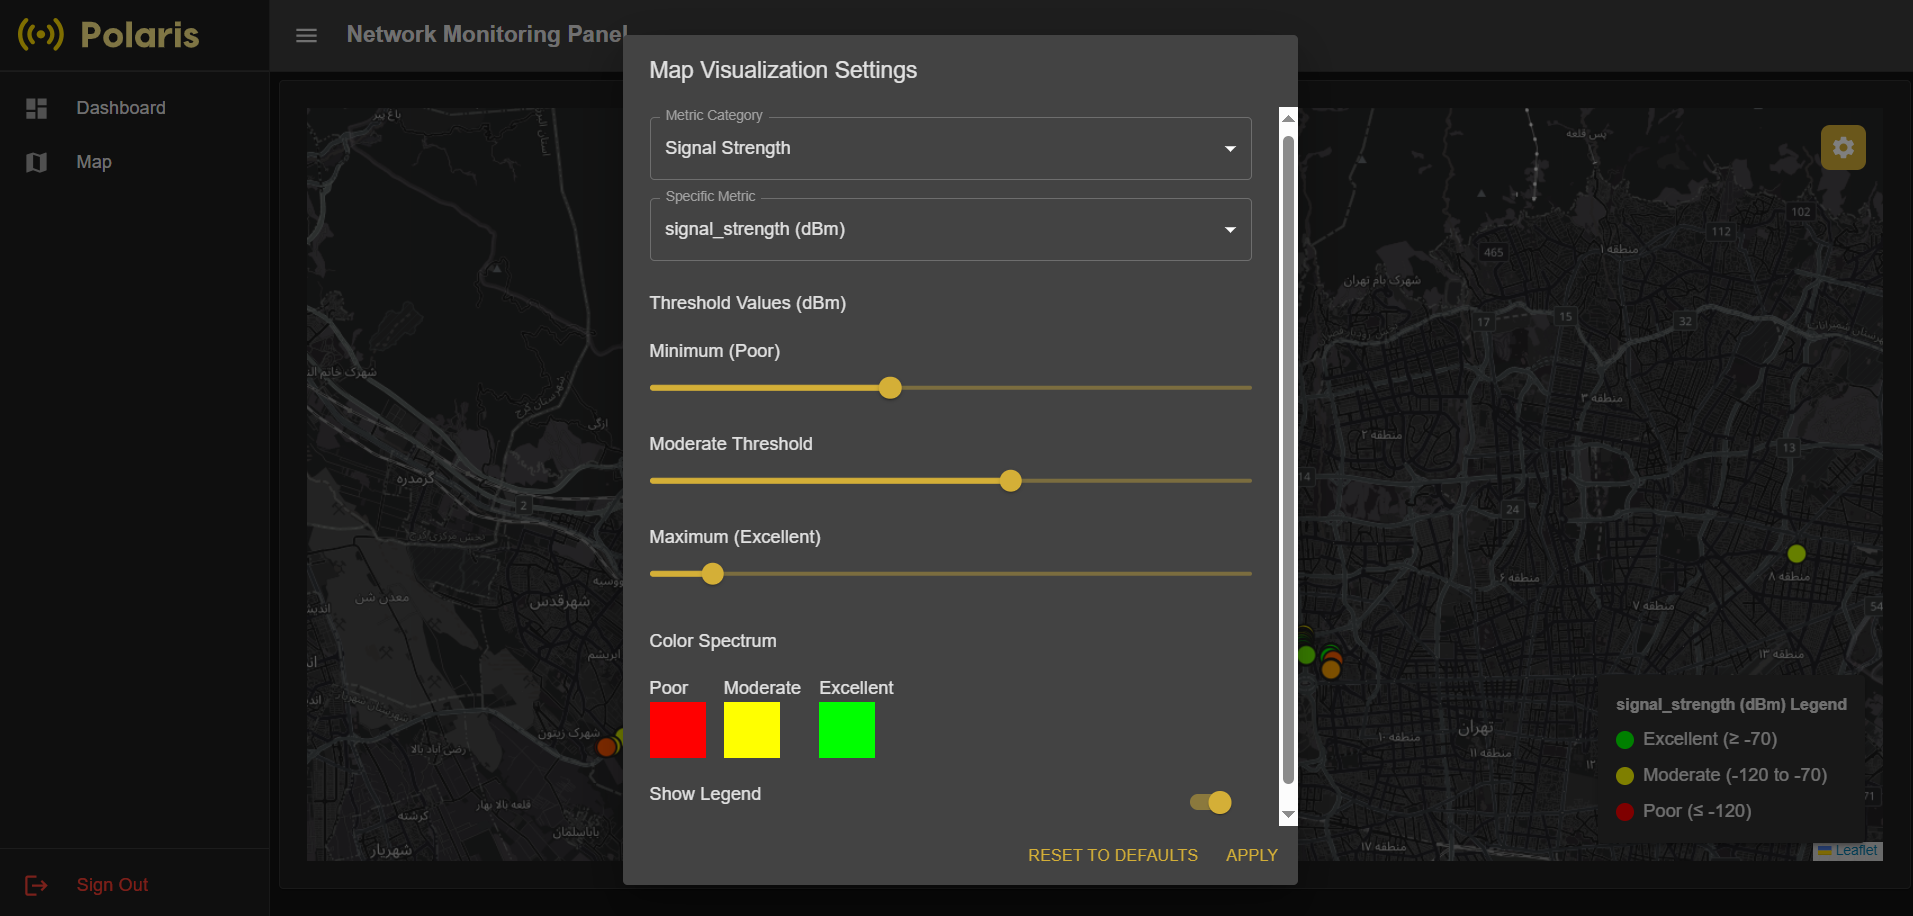
\includegraphics[width=\textwidth]{images/settings_overall.png}
    \end{center}

    \item در تصویر زیر، هر بخش از تنظیمات توضیح داده شده است:
    \begin{center}
        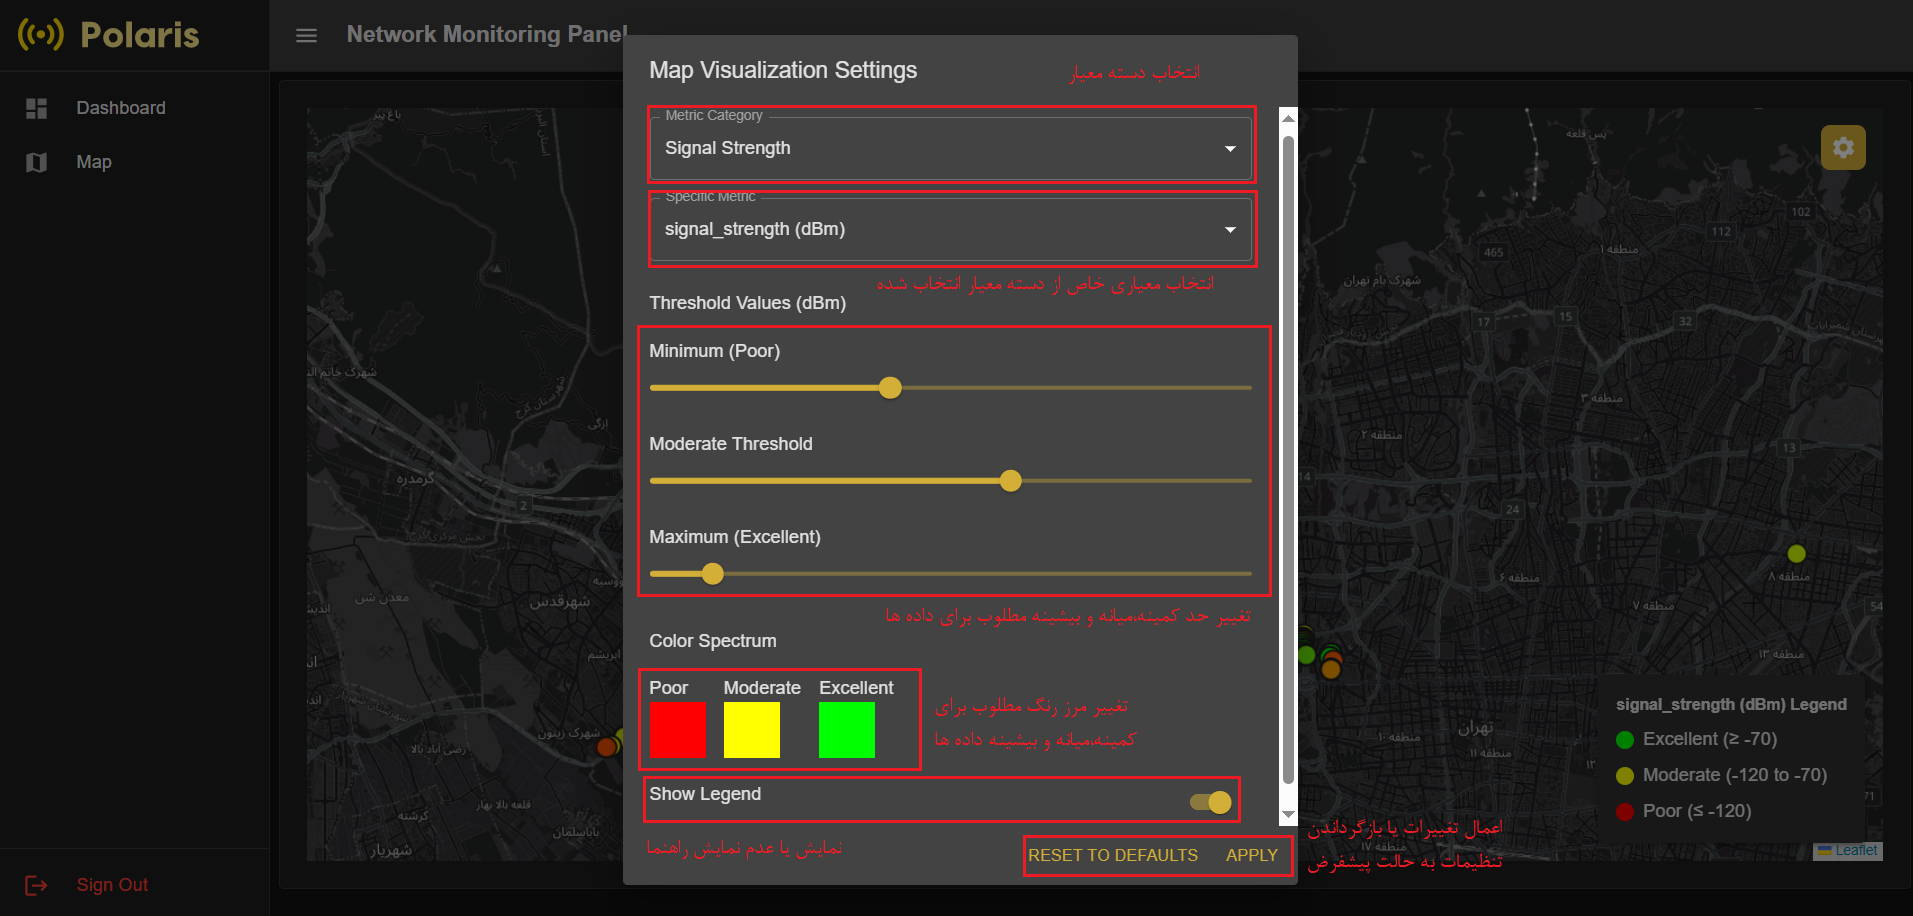
\includegraphics[width=\textwidth]{images/settings_overall_explained.png}
    \end{center}

    \item برای انتخاب معیار اصلی رنگ‌بندی، ابتدا دسته‌ی معیار را انتخاب کرده و سپس معیار مورد نظر را از آن دسته برگزینید.\\
    (برای معیارهای مربوط به قدرت سیگنال و کیفیت سیگنال، می‌توانید مقدار پیشفرض را انتخاب کنید تا مقادیر تمام نسل‌ها نمایش داده شوند.)
    \begin{center}
        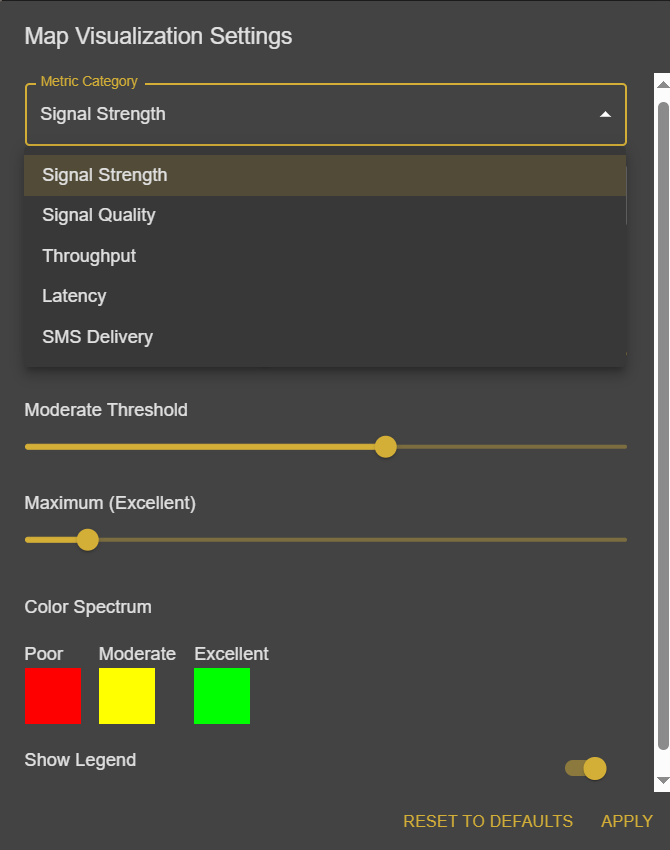
\includegraphics[width=\textwidth]{images/settings_metric_catagory.png}
    \end{center}
    \begin{center}
        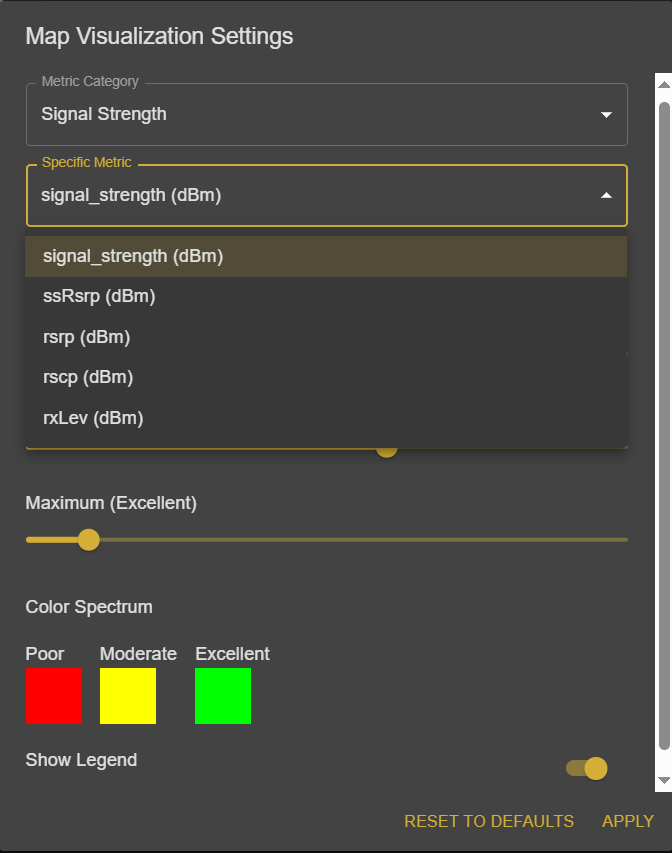
\includegraphics[width=\textwidth]{images/setting_signal_strength_metrics.png}
    \end{center}
    \begin{center}
        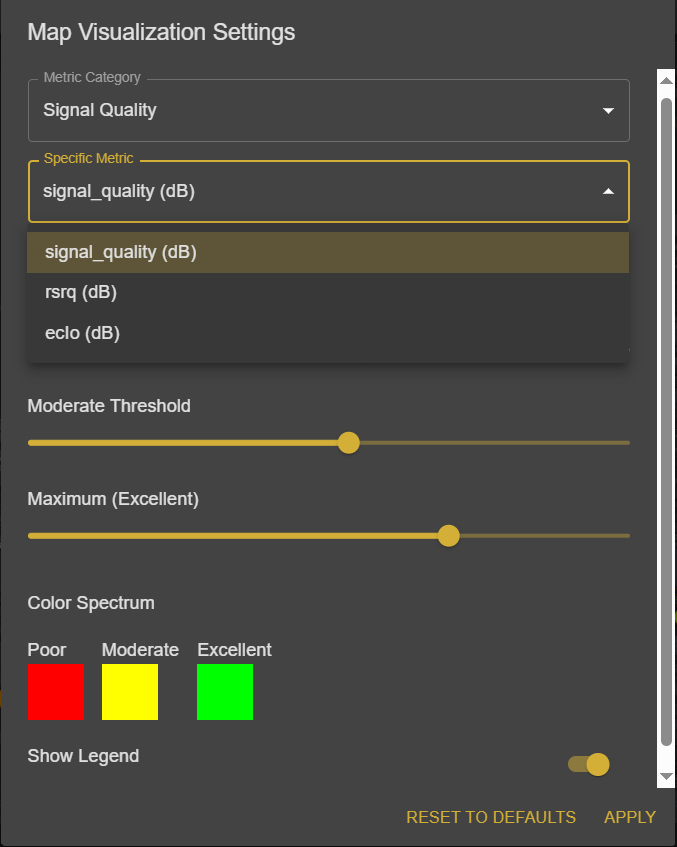
\includegraphics[width=\textwidth]{images/setting_signal_quality_metrics.png}
    \end{center}
    \begin{center}
        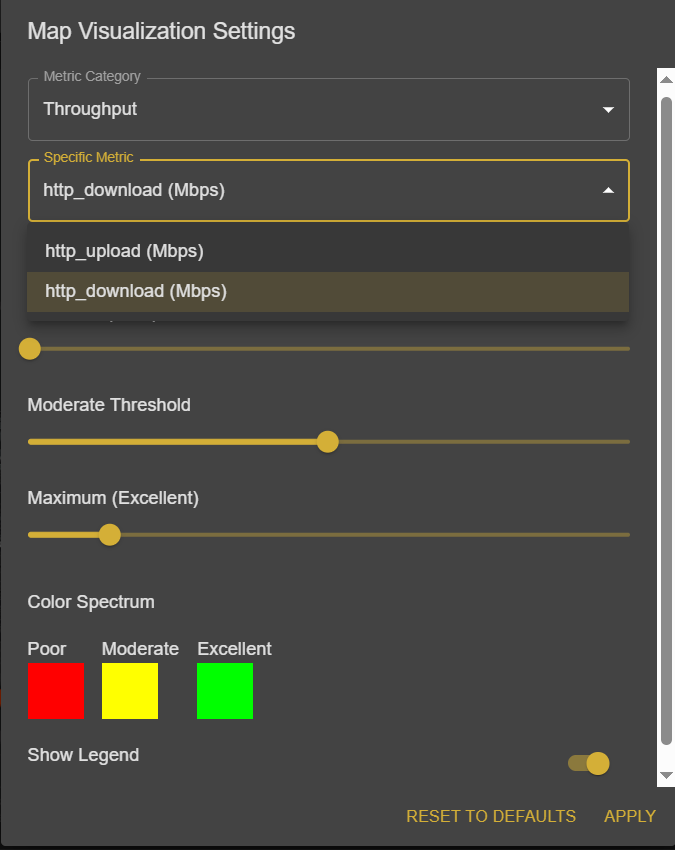
\includegraphics[width=\textwidth]{images/setting_throughput_metrics.png}
    \end{center}
    \begin{center}
        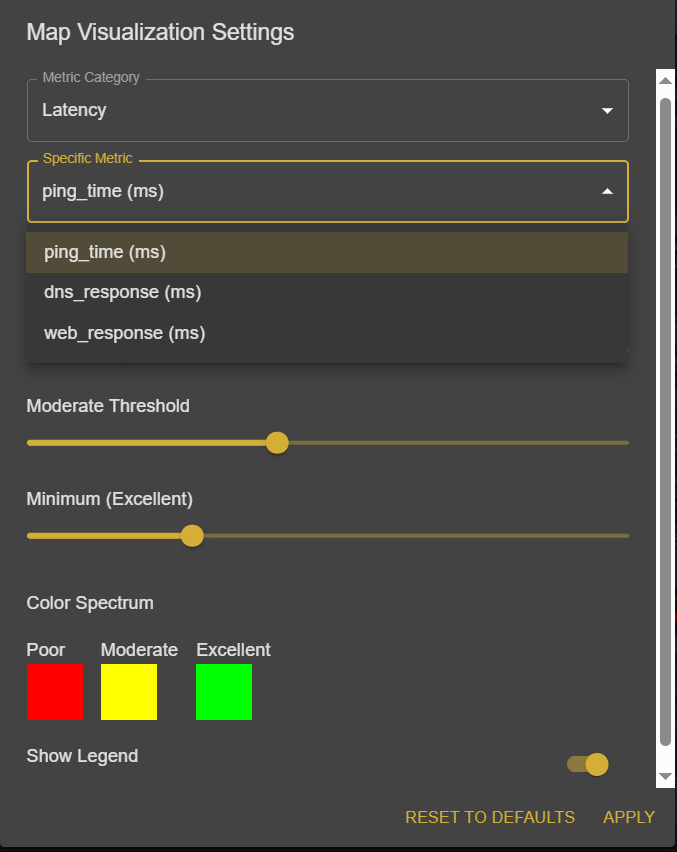
\includegraphics[width=\textwidth]{images/setting_latency_metrics.png}
    \end{center}
    \begin{center}
        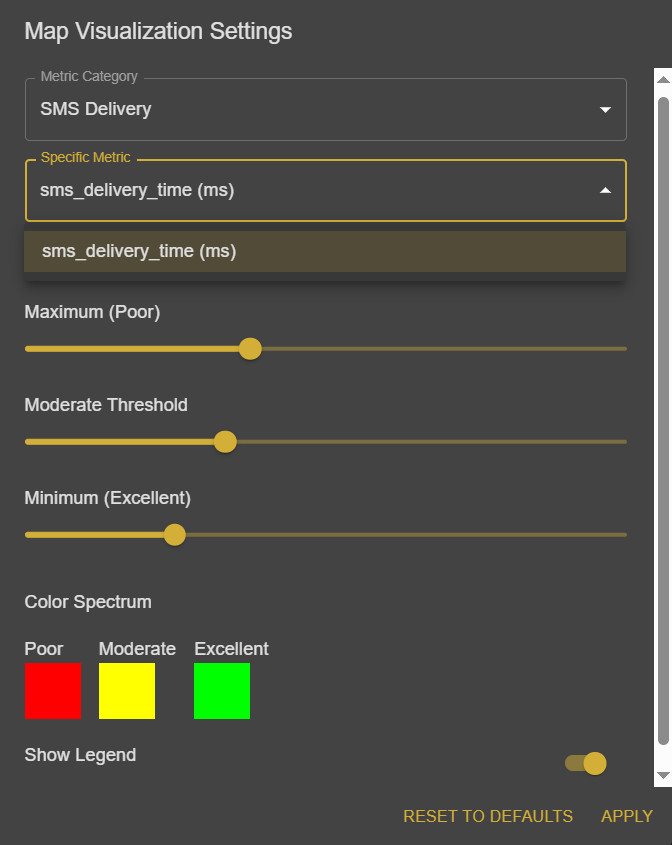
\includegraphics[width=\textwidth]{images/settings_sms_catagory.png}
    \end{center}

    \item در بخش میانی تنظیمات، چند \lr{Slider} وجود دارد که با استفاده از آنها می‌توان حداقل، میانه و حداکثر مقادیر مورد نظر برای گزارش‌ها را مشخص کرد.\\
    وجود \textbf{میانه} امکان نمایش غیرخطی طیف رنگ و شخصی‌سازی بهتر آن را فراهم می‌کند.\\
    \textbf{نکته:} ممکن است با تغییر یک \lr{Slider}، سایر \lr{Slider}‌ها نیز تغییر کنند. این رفتار طبیعی است، زیرا مقادیر دیگر برای هماهنگی با مقدار جدید تنظیم می‌شوند.

    \item در بخش پایینی \lr{Slider}ها می‌توان رنگ مرزی هر یک از بخش‌های حداقل، میانه و حداکثر را تعیین کرد.\\
    رنگ واقعی هر گزارش، طیفی بین این رنگ‌ها خواهد بود و بر اساس میزان نزدیکی مقدار گزارش به هر یک از این سطوح (حداقل، میانه و حداکثر) مشخص می‌شود.
    \begin{center}
        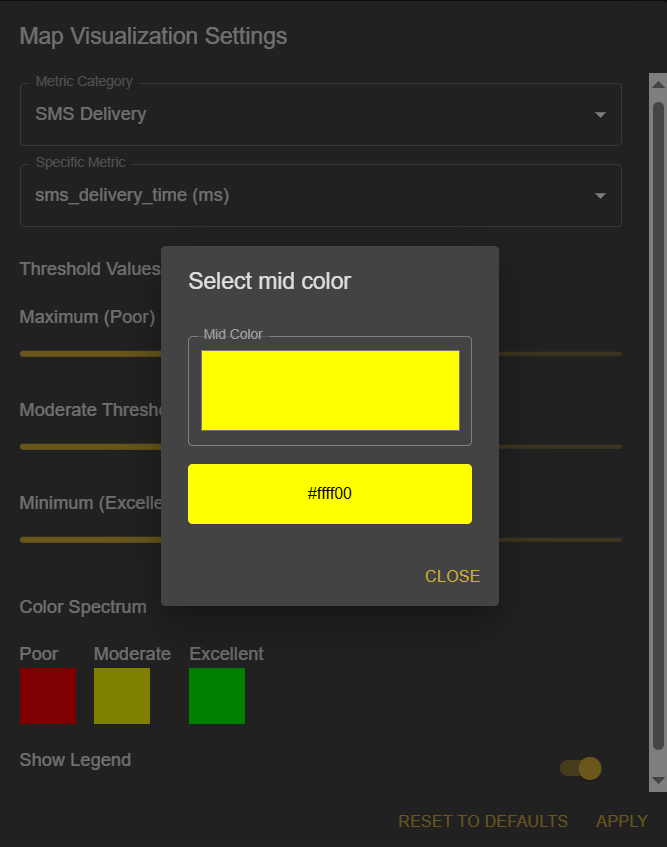
\includegraphics[width=\textwidth]{images/settings_color_picker.png}
    \end{center}

    \item در پایین تنظیمات، گزینه‌ای برای \textbf{خاموش کردن راهنما} وجود دارد تا بتوان دید بهتری از نقشه داشت (این قابلیت در نسخه‌ی موبایل بیشترین تأثیر را دارد).\\
    تصویر زیر نمونه‌ای از نقشه بدون راهنما است:
    \begin{center}
        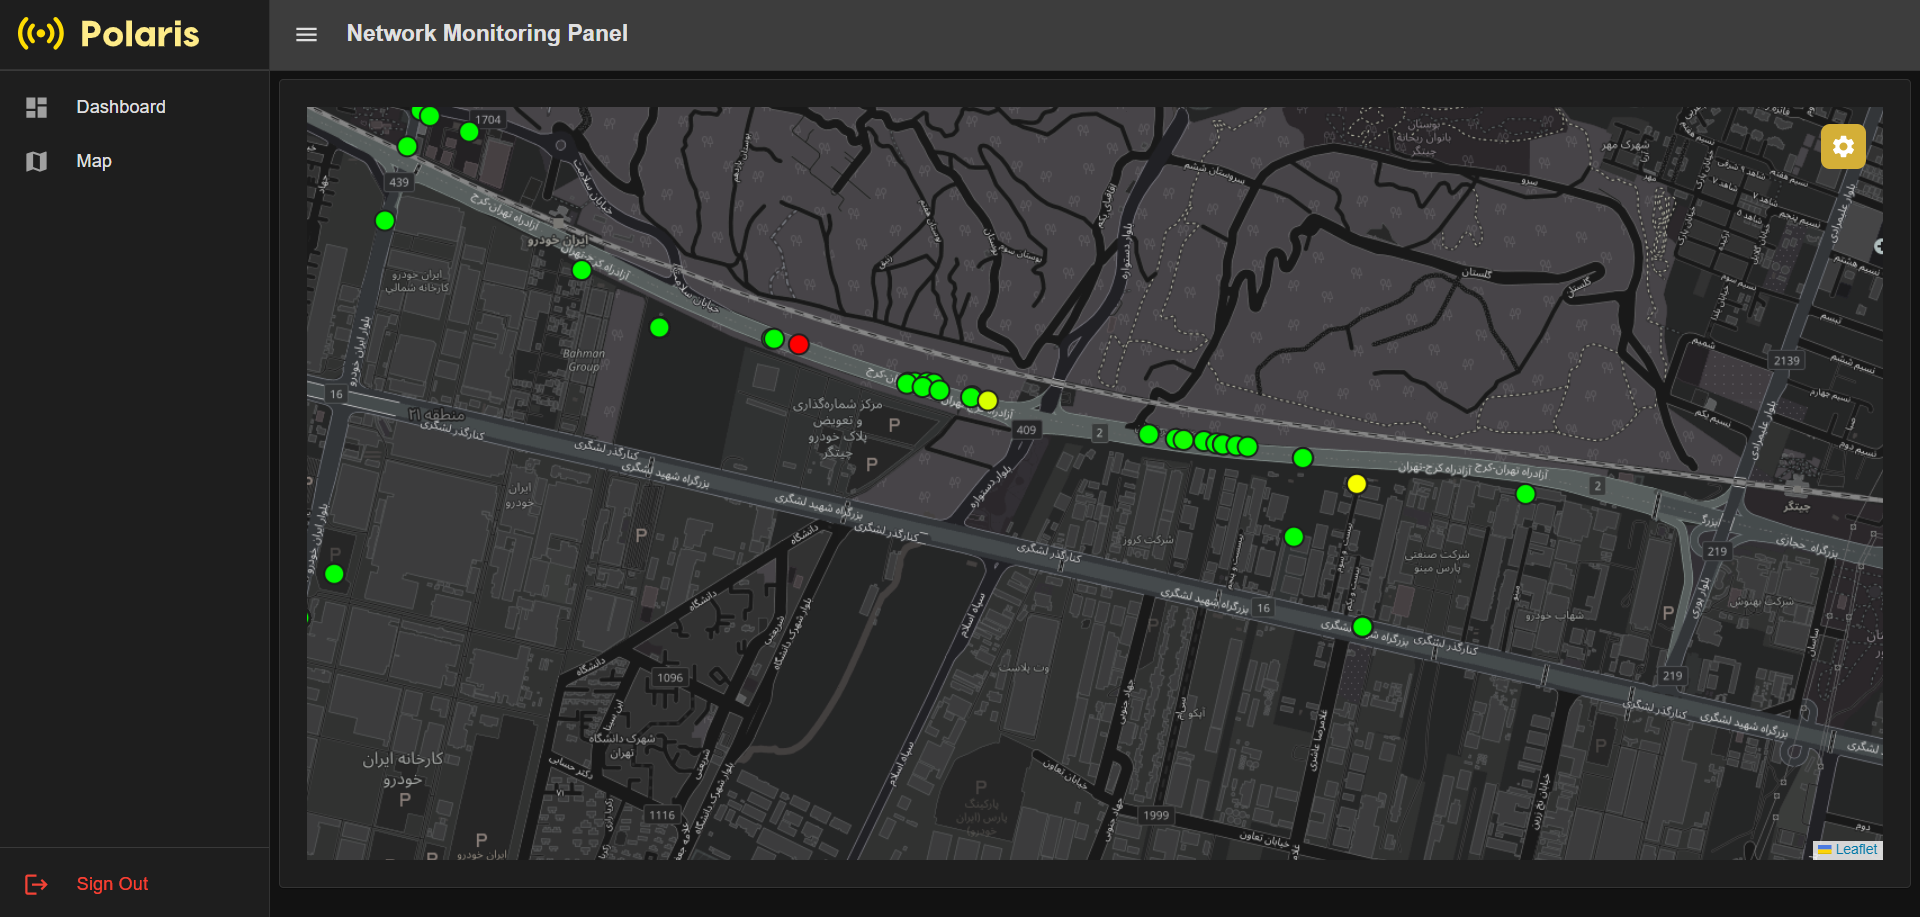
\includegraphics[width=\textwidth]{images/map_latency_legends_off.png}
    \end{center}

    \item اگر شما \textbf{کاربر ادمین} باشید، داده‌های تمام کاربران روی نقشه نمایش داده خواهند شد:
    \begin{center}
        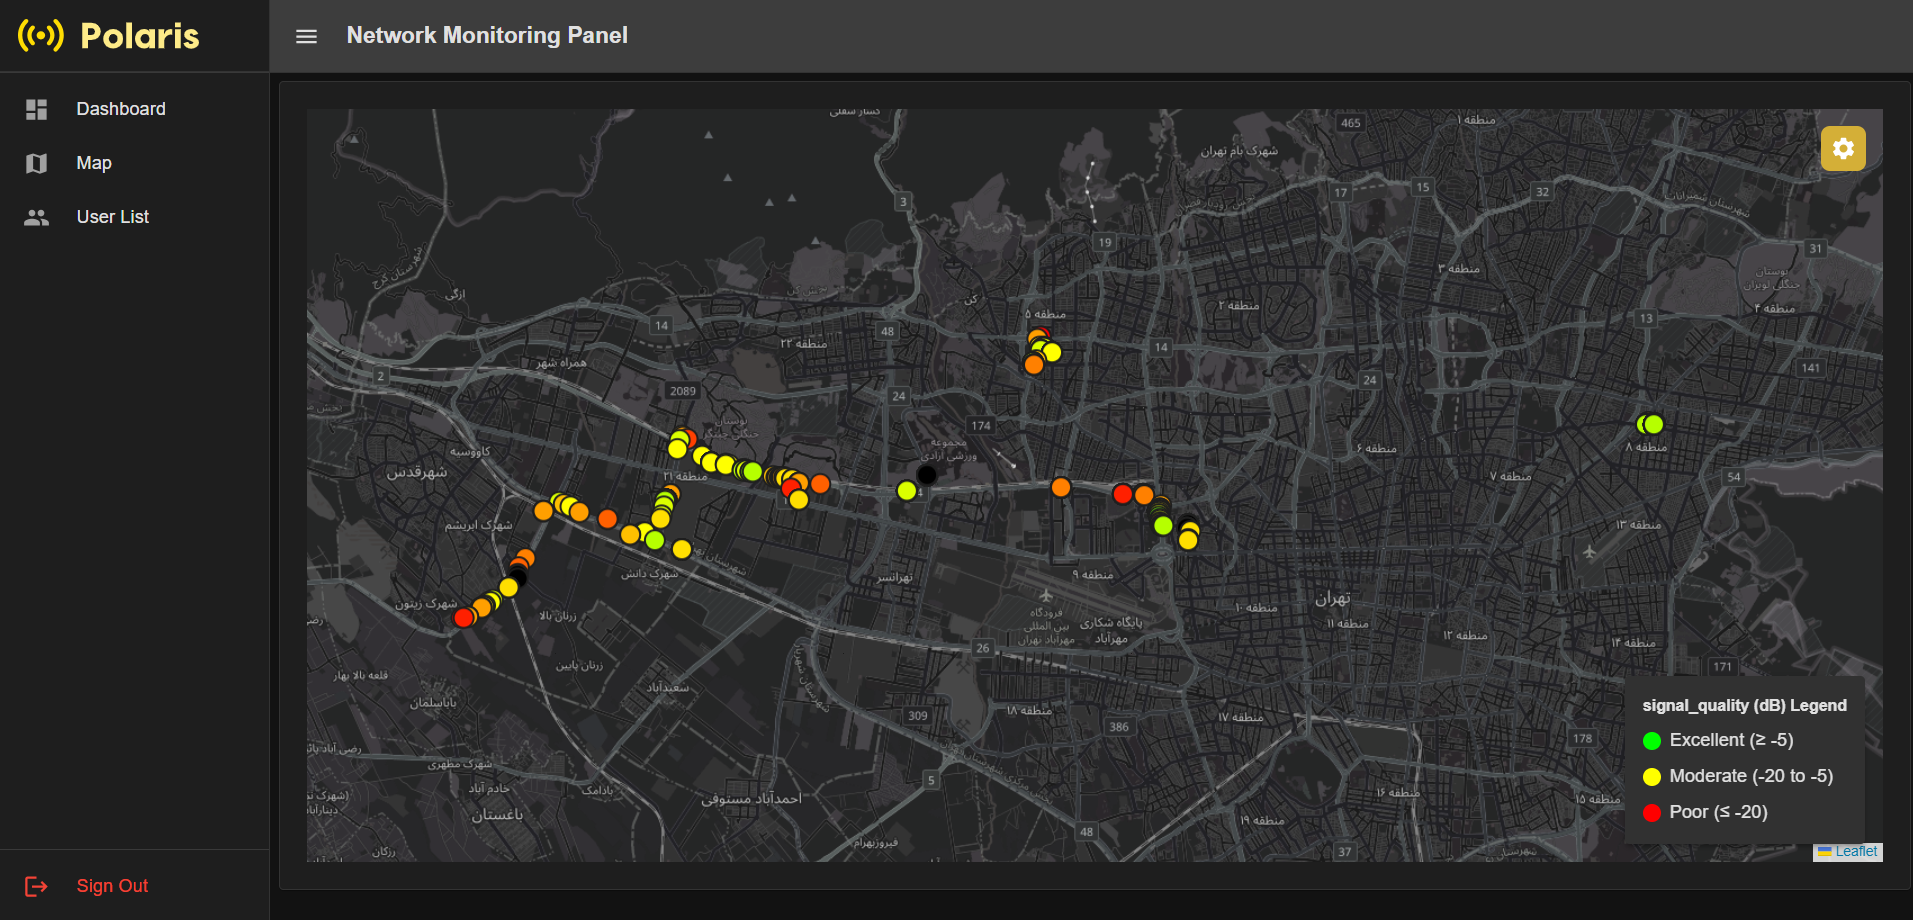
\includegraphics[width=\textwidth]{images/map_admin_all_data.png}
    \end{center}

    \item برای خاموش کردن این قابلیت، کافی است به تنظیمات رفته و گزینه‌ی \textbf{«نمایش داده‌ی همه‌ی کاربران»} را غیرفعال کنید.\\
    (این گزینه در پایین گزینه‌ی نمایش راهنما قرار دارد و فقط برای کاربران ادمین نمایش داده می‌شود.)
    \begin{center}
        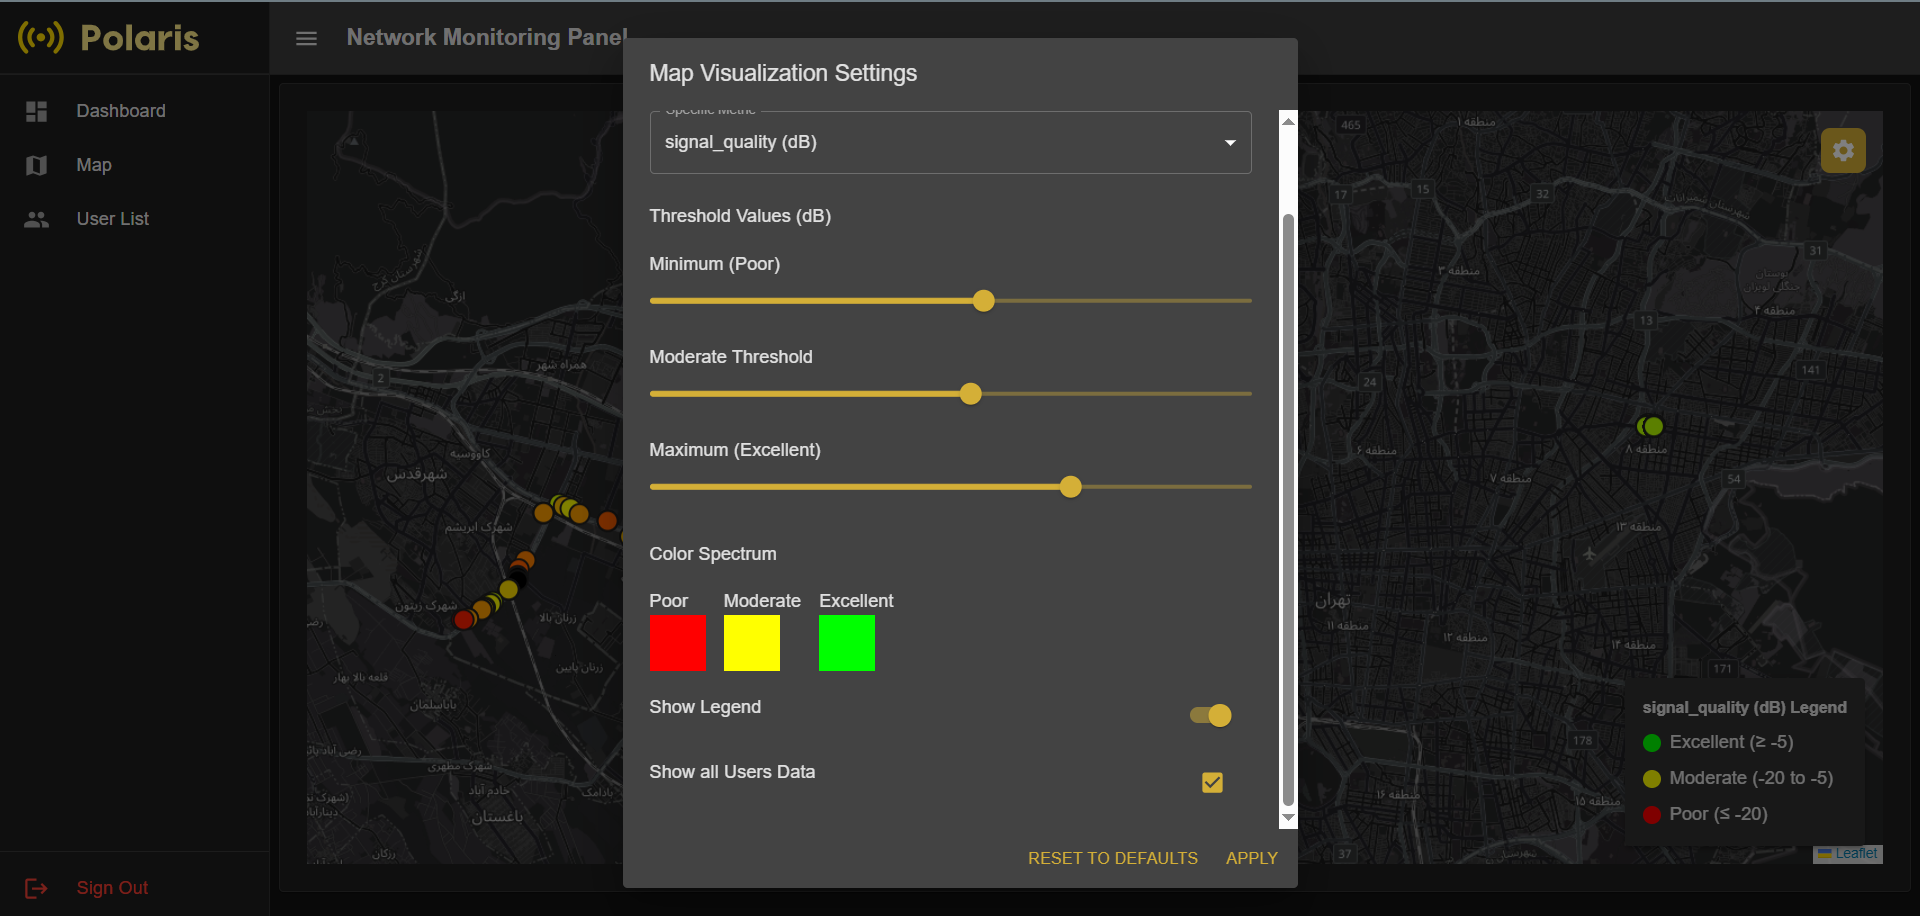
\includegraphics[width=\textwidth]{images/admin_settings_all_users_button.png}
    \end{center}
\end{itemize}
